% Options for packages loaded elsewhere
\PassOptionsToPackage{unicode}{hyperref}
\PassOptionsToPackage{hyphens}{url}
\PassOptionsToPackage{dvipsnames,svgnames,x11names}{xcolor}
%
\documentclass[
  letterpaper,
  DIV=11,
  numbers=noendperiod]{scrreprt}

\usepackage{amsmath,amssymb}
\usepackage{iftex}
\ifPDFTeX
  \usepackage[T1]{fontenc}
  \usepackage[utf8]{inputenc}
  \usepackage{textcomp} % provide euro and other symbols
\else % if luatex or xetex
  \usepackage{unicode-math}
  \defaultfontfeatures{Scale=MatchLowercase}
  \defaultfontfeatures[\rmfamily]{Ligatures=TeX,Scale=1}
\fi
\usepackage{lmodern}
\ifPDFTeX\else  
    % xetex/luatex font selection
\fi
% Use upquote if available, for straight quotes in verbatim environments
\IfFileExists{upquote.sty}{\usepackage{upquote}}{}
\IfFileExists{microtype.sty}{% use microtype if available
  \usepackage[]{microtype}
  \UseMicrotypeSet[protrusion]{basicmath} % disable protrusion for tt fonts
}{}
\makeatletter
\@ifundefined{KOMAClassName}{% if non-KOMA class
  \IfFileExists{parskip.sty}{%
    \usepackage{parskip}
  }{% else
    \setlength{\parindent}{0pt}
    \setlength{\parskip}{6pt plus 2pt minus 1pt}}
}{% if KOMA class
  \KOMAoptions{parskip=half}}
\makeatother
\usepackage{xcolor}
\setlength{\emergencystretch}{3em} % prevent overfull lines
\setcounter{secnumdepth}{5}
% Make \paragraph and \subparagraph free-standing
\makeatletter
\ifx\paragraph\undefined\else
  \let\oldparagraph\paragraph
  \renewcommand{\paragraph}{
    \@ifstar
      \xxxParagraphStar
      \xxxParagraphNoStar
  }
  \newcommand{\xxxParagraphStar}[1]{\oldparagraph*{#1}\mbox{}}
  \newcommand{\xxxParagraphNoStar}[1]{\oldparagraph{#1}\mbox{}}
\fi
\ifx\subparagraph\undefined\else
  \let\oldsubparagraph\subparagraph
  \renewcommand{\subparagraph}{
    \@ifstar
      \xxxSubParagraphStar
      \xxxSubParagraphNoStar
  }
  \newcommand{\xxxSubParagraphStar}[1]{\oldsubparagraph*{#1}\mbox{}}
  \newcommand{\xxxSubParagraphNoStar}[1]{\oldsubparagraph{#1}\mbox{}}
\fi
\makeatother

\usepackage{color}
\usepackage{fancyvrb}
\newcommand{\VerbBar}{|}
\newcommand{\VERB}{\Verb[commandchars=\\\{\}]}
\DefineVerbatimEnvironment{Highlighting}{Verbatim}{commandchars=\\\{\}}
% Add ',fontsize=\small' for more characters per line
\newenvironment{Shaded}{}{}
\newcommand{\AlertTok}[1]{\textcolor[rgb]{1.00,0.33,0.33}{\textbf{#1}}}
\newcommand{\AnnotationTok}[1]{\textcolor[rgb]{0.42,0.45,0.49}{#1}}
\newcommand{\AttributeTok}[1]{\textcolor[rgb]{0.84,0.23,0.29}{#1}}
\newcommand{\BaseNTok}[1]{\textcolor[rgb]{0.00,0.36,0.77}{#1}}
\newcommand{\BuiltInTok}[1]{\textcolor[rgb]{0.84,0.23,0.29}{#1}}
\newcommand{\CharTok}[1]{\textcolor[rgb]{0.01,0.18,0.38}{#1}}
\newcommand{\CommentTok}[1]{\textcolor[rgb]{0.42,0.45,0.49}{#1}}
\newcommand{\CommentVarTok}[1]{\textcolor[rgb]{0.42,0.45,0.49}{#1}}
\newcommand{\ConstantTok}[1]{\textcolor[rgb]{0.00,0.36,0.77}{#1}}
\newcommand{\ControlFlowTok}[1]{\textcolor[rgb]{0.84,0.23,0.29}{#1}}
\newcommand{\DataTypeTok}[1]{\textcolor[rgb]{0.84,0.23,0.29}{#1}}
\newcommand{\DecValTok}[1]{\textcolor[rgb]{0.00,0.36,0.77}{#1}}
\newcommand{\DocumentationTok}[1]{\textcolor[rgb]{0.42,0.45,0.49}{#1}}
\newcommand{\ErrorTok}[1]{\textcolor[rgb]{1.00,0.33,0.33}{\underline{#1}}}
\newcommand{\ExtensionTok}[1]{\textcolor[rgb]{0.84,0.23,0.29}{\textbf{#1}}}
\newcommand{\FloatTok}[1]{\textcolor[rgb]{0.00,0.36,0.77}{#1}}
\newcommand{\FunctionTok}[1]{\textcolor[rgb]{0.44,0.26,0.76}{#1}}
\newcommand{\ImportTok}[1]{\textcolor[rgb]{0.01,0.18,0.38}{#1}}
\newcommand{\InformationTok}[1]{\textcolor[rgb]{0.42,0.45,0.49}{#1}}
\newcommand{\KeywordTok}[1]{\textcolor[rgb]{0.84,0.23,0.29}{#1}}
\newcommand{\NormalTok}[1]{\textcolor[rgb]{0.14,0.16,0.18}{#1}}
\newcommand{\OperatorTok}[1]{\textcolor[rgb]{0.14,0.16,0.18}{#1}}
\newcommand{\OtherTok}[1]{\textcolor[rgb]{0.44,0.26,0.76}{#1}}
\newcommand{\PreprocessorTok}[1]{\textcolor[rgb]{0.84,0.23,0.29}{#1}}
\newcommand{\RegionMarkerTok}[1]{\textcolor[rgb]{0.42,0.45,0.49}{#1}}
\newcommand{\SpecialCharTok}[1]{\textcolor[rgb]{0.00,0.36,0.77}{#1}}
\newcommand{\SpecialStringTok}[1]{\textcolor[rgb]{0.01,0.18,0.38}{#1}}
\newcommand{\StringTok}[1]{\textcolor[rgb]{0.01,0.18,0.38}{#1}}
\newcommand{\VariableTok}[1]{\textcolor[rgb]{0.89,0.38,0.04}{#1}}
\newcommand{\VerbatimStringTok}[1]{\textcolor[rgb]{0.01,0.18,0.38}{#1}}
\newcommand{\WarningTok}[1]{\textcolor[rgb]{1.00,0.33,0.33}{#1}}

\providecommand{\tightlist}{%
  \setlength{\itemsep}{0pt}\setlength{\parskip}{0pt}}\usepackage{longtable,booktabs,array}
\usepackage{calc} % for calculating minipage widths
% Correct order of tables after \paragraph or \subparagraph
\usepackage{etoolbox}
\makeatletter
\patchcmd\longtable{\par}{\if@noskipsec\mbox{}\fi\par}{}{}
\makeatother
% Allow footnotes in longtable head/foot
\IfFileExists{footnotehyper.sty}{\usepackage{footnotehyper}}{\usepackage{footnote}}
\makesavenoteenv{longtable}
\usepackage{graphicx}
\makeatletter
\newsavebox\pandoc@box
\newcommand*\pandocbounded[1]{% scales image to fit in text height/width
  \sbox\pandoc@box{#1}%
  \Gscale@div\@tempa{\textheight}{\dimexpr\ht\pandoc@box+\dp\pandoc@box\relax}%
  \Gscale@div\@tempb{\linewidth}{\wd\pandoc@box}%
  \ifdim\@tempb\p@<\@tempa\p@\let\@tempa\@tempb\fi% select the smaller of both
  \ifdim\@tempa\p@<\p@\scalebox{\@tempa}{\usebox\pandoc@box}%
  \else\usebox{\pandoc@box}%
  \fi%
}
% Set default figure placement to htbp
\def\fps@figure{htbp}
\makeatother

\usepackage{booktabs}
\usepackage{longtable}
\usepackage{array}
\usepackage{multirow}
\usepackage{wrapfig}
\usepackage{float}
\usepackage{colortbl}
\usepackage{pdflscape}
\usepackage{tabu}
\usepackage{threeparttable}
\usepackage{threeparttablex}
\usepackage[normalem]{ulem}
\usepackage{makecell}
\usepackage{xcolor}
\usepackage{fvextra}
\DefineVerbatimEnvironment{Highlighting}{Verbatim}{breaklines,commandchars=\\\{\}}
\DefineVerbatimEnvironment{OutputCode}{Verbatim}{breaklines,commandchars=\\\{\}}
\KOMAoption{captions}{tableheading}
\makeatletter
\@ifpackageloaded{bookmark}{}{\usepackage{bookmark}}
\makeatother
\makeatletter
\@ifpackageloaded{caption}{}{\usepackage{caption}}
\AtBeginDocument{%
\ifdefined\contentsname
  \renewcommand*\contentsname{Table of contents}
\else
  \newcommand\contentsname{Table of contents}
\fi
\ifdefined\listfigurename
  \renewcommand*\listfigurename{List of Figures}
\else
  \newcommand\listfigurename{List of Figures}
\fi
\ifdefined\listtablename
  \renewcommand*\listtablename{List of Tables}
\else
  \newcommand\listtablename{List of Tables}
\fi
\ifdefined\figurename
  \renewcommand*\figurename{Figure}
\else
  \newcommand\figurename{Figure}
\fi
\ifdefined\tablename
  \renewcommand*\tablename{Table}
\else
  \newcommand\tablename{Table}
\fi
}
\@ifpackageloaded{float}{}{\usepackage{float}}
\floatstyle{ruled}
\@ifundefined{c@chapter}{\newfloat{codelisting}{h}{lop}}{\newfloat{codelisting}{h}{lop}[chapter]}
\floatname{codelisting}{Listing}
\newcommand*\listoflistings{\listof{codelisting}{List of Listings}}
\makeatother
\makeatletter
\makeatother
\makeatletter
\@ifpackageloaded{caption}{}{\usepackage{caption}}
\@ifpackageloaded{subcaption}{}{\usepackage{subcaption}}
\makeatother

\usepackage[]{biblatex}
\addbibresource{bibliography.bib}
\usepackage{bookmark}

\IfFileExists{xurl.sty}{\usepackage{xurl}}{} % add URL line breaks if available
\urlstyle{same} % disable monospaced font for URLs
\hypersetup{
  pdftitle={Mutation Load in Black Grouse},
  pdfauthor={Rebecca S. Chen},
  colorlinks=true,
  linkcolor={blue},
  filecolor={Maroon},
  citecolor={Blue},
  urlcolor={Blue},
  pdfcreator={LaTeX via pandoc}}


\title{Mutation Load in Black Grouse}
\author{Rebecca S. Chen}
\date{}

\begin{document}
\maketitle

\renewcommand*\contentsname{Table of contents}
{
\hypersetup{linkcolor=}
\setcounter{tocdepth}{1}
\tableofcontents
}

\bookmarksetup{startatroot}

\chapter{Mutation load in black
grouse}\label{mutation-load-in-black-grouse}

\bookmarksetup{startatroot}

\chapter{Introduction}\label{introduction}

This webpage/document contains a summary of the workflow used in the
manuscript titled ``\textbf{Genetic architecture of male reproductive
success in a lekking bird: insights from predicted deleterious
mutations}'', Chen et al.~2024
(\href{https://doi.org/10.21203/rs.3.rs-5579350/v1}{in review}). Please
see the \href{https://github.com/rshuhuachen/ms_load_grouse}{github
repository} for all scripts and more detailed descriptions of the data
and analyses.

\begin{figure}[H]

{\centering \pandocbounded{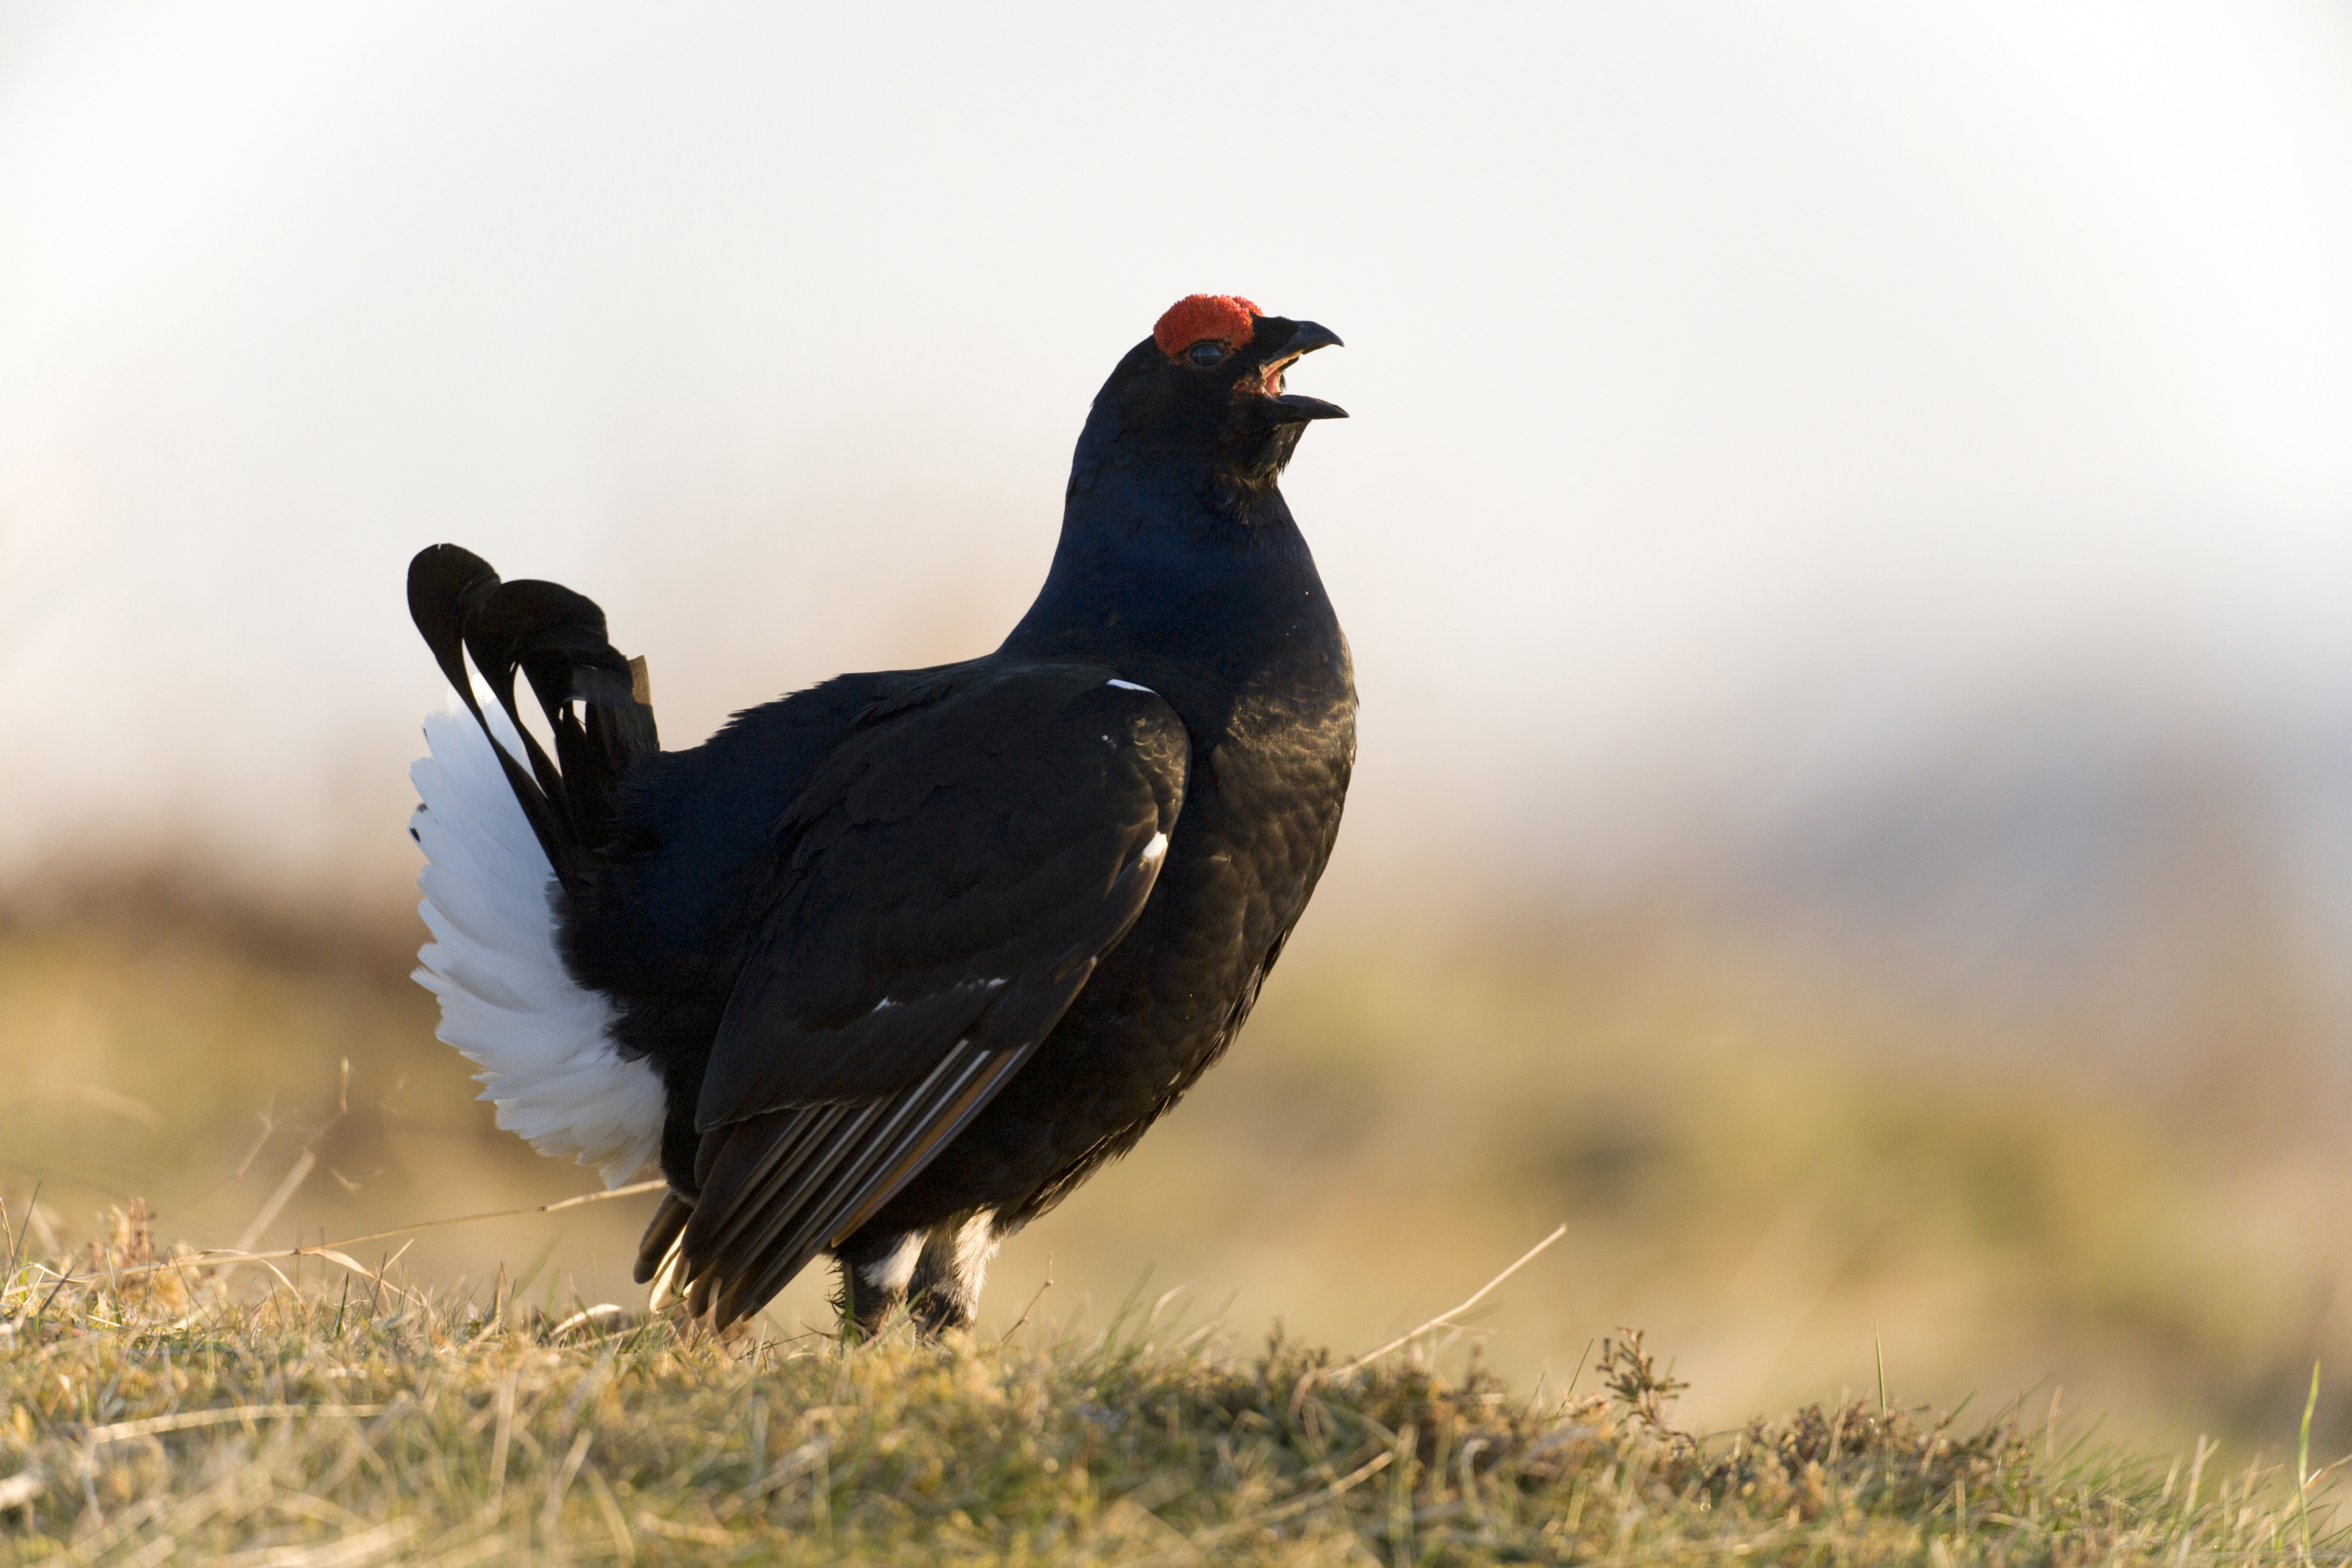
\includegraphics[keepaspectratio]{plots/img/grouse.jpeg}}

}

\caption{Black grouse}

\end{figure}%

\bookmarksetup{startatroot}

\chapter{Main goals}\label{main-goals}

In the current study, we used a long-term dataset to (i) quantify the
fitness effects of total, homozygous and heterozygous individual genomic
mutation loads; (ii) evaluate the relative contributions of deleterious
mutations across different genomic regions and biological processes to
fitness variation (iii) unravel the behavioural and / or ornamental
pathways through which deleterious mutations impact lifetime
reproductive success. We used whole genome resequencing, phenotypic and
fitness data of 190 male black grouse sampled annually across five study
sites in Central

Mutation load can be defined as a statistic that summarizes the
selection and dominance coefficients of deleterious mutations as a
function of their frequencies in a population
\autocite{bertorelleGeneticLoadGenomic2022}. As we do not have selection
and dominance coefficients of mutations in wild populations, we use a
proxy for mutation load calculated as the number of deleterious
mutations for a given individual.

There are different types of load, e.g.~the realized load (expressed
load) which reduces fitness in the current generation, and the
potential/masked load (inbreeding load) which quantifies the potential
fitness loss due to (partially) recessive deleterious mutations that may
become expressed in future generations depending on the population's
demography. The genetic load is made up of realized plus masked load.

\bookmarksetup{startatroot}

\chapter{Calculating genetic load}\label{calculating-genetic-load}

There are generally two most commonly used computational approaches to
identify putative deleterious variants from whole genome re-sequencing
data. In general, these tools attempt to predict the effect of a
mutation on the function or evolutionary fitness of a protein. The two
are distinct but can be related; for instance, a loss of function
mutation will be strongly selected against if the gene is essential but
will tend to be less evolutionary deleterious if the gene is
non-essential or if the variant only slightly alters protein function.
We used two common approaches:

\begin{itemize}
\item
  Genomic Evolutionary Rate Profiling (GERP): This approach uses
  multi-species genome alignments to identify genomic sites that are
  strongly conserved over millions of years of evolution, as
  non-synonymous mutations at these sites have a high likelihood of
  being deleterious. \autocite{davydovIdentifyingHighFraction2010}
\item
  SNP effect (SnpEff): This approach predicts the consequences of
  genomic variants on protein sequences and identifies loss of function
  and missense variants. \autocite{cingolani2012}.
\end{itemize}

\bookmarksetup{startatroot}

\chapter{This webpage / document}\label{this-webpage-document}

This \href{https://rshuhuachen.github.io/ms_load_grouse/}{webpage} can
also be found in
\href{https://github.com/rshuhuachen/ms_load_grouse/docs/Mutation-Load-in-Black-Grouse.pdf}{PDF
format} on github. Note that in the PDF format, code is not folded which
will end up in a lengthy document, and the html looks aesthetically
better ;). In both documents, you will find some of the scripts for the
analysis performed in this study. Note that not all bioinformatic steps
are put on here (only from inferring mutations onwards). You can find
the complete set of analyses with their explanations in the github repo.

\bookmarksetup{startatroot}

\chapter{SnpEff}\label{snpeff}

\section{Introduction}\label{introduction-1}

\href{https://pcingola.github.io/SnpEff/}{SnpEff} annotates genetic
variants and predicts the functional effects. The output includes a VCF
file with annotations that indicate what kind of mutation it is
(e.g.~introduction of a stop codon) and the predicted effect (low,
moderate, high, modifier). In this study, we focus on high impact
mutations, which include loss of function (LoF) and nonsense mediate
decay (NMD) mutations.

\section{Methods}\label{methods}

\subsection{Building the database}\label{building-the-database}

As the black grouse (\emph{Lyrurus tetrix}) is no common model species
with a pre-built database, a custom database was built from the
annotation files in .gff format provided by Cantata Bio.

To build a custom database, five files are required: the gff file
containing the gene annotation, the reference genome, and then three
files containing information about the coding regions (cds.fa; a fasta
file containing the coding regions only), the genes (genes.fa; a fasta
file containing the genes only) and a file with the protein sequences
(proteins.fa; a fasta file with the protein sequences). Two softwares
were used to construct these three fasta files: gff3\_to\_fasta and
AGAT.

\begin{Shaded}
\begin{Highlighting}[]
\NormalTok{gff3\_to\_fasta {-}g data/genomic/refgenome/PO2979\_Lyrurus\_tetrix\_black\_grouse.annotation.gff \textbackslash{}}
\NormalTok{    {-}f data/genomic/refgenome/PO2979\_Lyrurus\_tetrix\_black\_grouse.RepeatMasked.fasta {-}st cds {-}d complete {-}o data/genomic/refgenome/lyrurus\_tetrix/cds.fa }

\NormalTok{gff3\_to\_fasta {-}g data/genomic/refgenome/PO2979\_Lyrurus\_tetrix\_black\_grouse.annotation.gff \textbackslash{}}
\NormalTok{    {-}f data/genomic/refgenome/PO2979\_Lyrurus\_tetrix\_black\_grouse.RepeatMasked.fasta {-}st gene {-}d complete {-}o data/genomic/refgenome/lyrurus\_tetrix/genes.fa }
\end{Highlighting}
\end{Shaded}

Similarly, the protein sequences were constructed with AGAT

\begin{Shaded}
\begin{Highlighting}[]
\NormalTok{agat\_sp\_extract\_sequences.pl {-}{-}gff data/genomic/refgenome/PO2979\_Lyrurus\_tetrix\_black\_grouse.annotation.gff {-}f \textbackslash{}}
\NormalTok{    data/genomic/refgenome/PO2979\_Lyrurus\_tetrix\_black\_grouse.RepeatMasked.fasta {-}p {-}o \textbackslash{}}
\NormalTok{    data/genomic/refgenome/lyrurus\_tetrix/protein.fa}
\end{Highlighting}
\end{Shaded}

Then, the database was built (and automatically checked).

\begin{Shaded}
\begin{Highlighting}[]
\NormalTok{java {-}jar snpEff.jar build {-}gff3 {-}v data/genomic/refgenome/lyrurus\_tetrix}
\end{Highlighting}
\end{Shaded}

Once the database is ready, we can run SnpEff to create the annotated
vcf file.

\begin{Shaded}
\begin{Highlighting}[]
\NormalTok{java {-}Xmx8g {-}jar snpEff.jar ann {-}stats  \textbackslash{}}
\NormalTok{{-}no{-}downstream {-}no{-}intergenic {-}no{-}intron {-}no{-}upstream {-}no{-}utr {-}v \textbackslash{}}
\NormalTok{lyrurus\_tetrix data/genomic/intermediate/ltet\_snps\_filtered.vcf \textgreater{} data/genomic/intermediate/snpef/ltet\_ann\_snp\_output.vcf}
\end{Highlighting}
\end{Shaded}

\subsection{Ancestral alleles}\label{ancestral-alleles}

SnpEff annotates mutations according to the change from the reference
allele to the focal allele. Hence, it assumes that the reference allele
is the `better' one and that a mutation that changes the transcription
of this reference allele is detrimental. To allow this assumption to be
better met, we used the ancestral genome as a reference, instead of the
reference genome itself (i.e.~we polarized the genome). This ancestral
genome is constructed by cactus, and represents the most recent common
ancestor between black grouse \emph{(L. tetrix)} and \emph{Lagoplus
leucura} (white tailed ptarmigan). This way, any derived allele was
assumed to be `deleterious' compared to the ancestral allele, as opposed
to a reference-non reference comparison.

\subsection{Filtering}\label{filtering}

We then used SnpSift to filter annotated mutations based on the four
impact categories: modifier, low, moderate and
\href{https://pcingola.github.io/SnpEff/se_inputoutput/\#effect-prediction-details}{high
impact} using the following commands.

\begin{Shaded}
\begin{Highlighting}[]

\NormalTok{\#\# High impact}
\NormalTok{zcat output/ancestral/ltet\_filtered\_ann\_aa.vcf.gz | java {-}jar src/SnpSift.jar filter " ( ANN[*].IMPACT = \textquotesingle{}HIGH\textquotesingle{} )" \textgreater{} data/genomic/intermediate/snpef/ltet\_ann\_aa\_snp\_output\_HIGH.vcf}
\NormalTok{gzip data/genomic/intermediate/snpef/ltet\_ann\_aa\_snp\_output\_HIGH.vcf}

\NormalTok{\#\# Moderate}
\NormalTok{zcat output/ancestral/ltet\_filtered\_ann\_aa.vcf.gz | java {-}jar src/SnpSift.jar filter " ( ANN[*].IMPACT = \textquotesingle{}MODERATE\textquotesingle{})" \textgreater{} data/genomic/intermediate/snpef/ltet\_ann\_aa\_snp\_output\_moderate.vcf}
\NormalTok{gzip data/genomic/intermediate/snpef/ltet\_ann\_aa\_snp\_output\_moderate.vcf}

\NormalTok{\#\# Low}
\NormalTok{zcat output/ancestral/ltet\_filtered\_ann\_aa.vcf.gz | java {-}jar src/SnpSift.jar filter " ( ANN[*].IMPACT = \textquotesingle{}LOW\textquotesingle{}) " \textgreater{} data/genomic/intermediate/snpef/ltet\_ann\_aa\_snp\_output\_low.vcf}
\NormalTok{gzip data/genomic/intermediate/snpef/ltet\_ann\_aa\_snp\_output\_low.vcf}
\end{Highlighting}
\end{Shaded}

\section{Results}\label{results}

We identified 5,341 high impact mutations:

\begin{figure}[H]

{\centering \pandocbounded{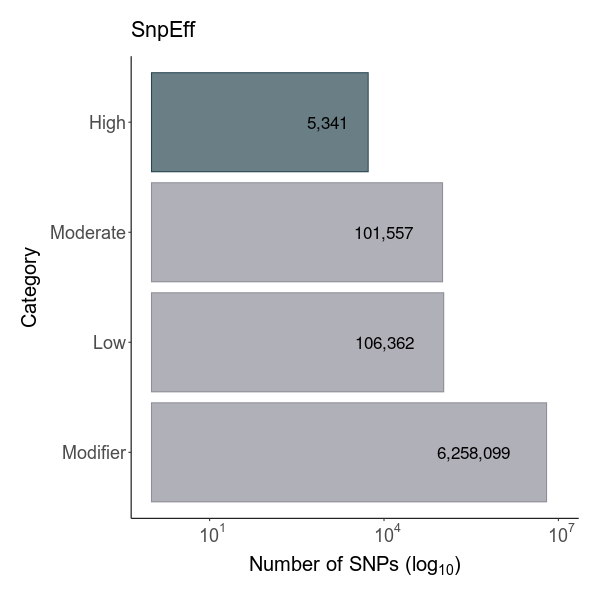
\includegraphics[keepaspectratio]{qmd/../plots/main/fig_1b.png}}

}

\caption{SnpEff annotation}

\end{figure}%

Existing of mostly LoF mutations and gained stop codons (non-mutually
exclusive)

\begin{figure}[H]

{\centering \pandocbounded{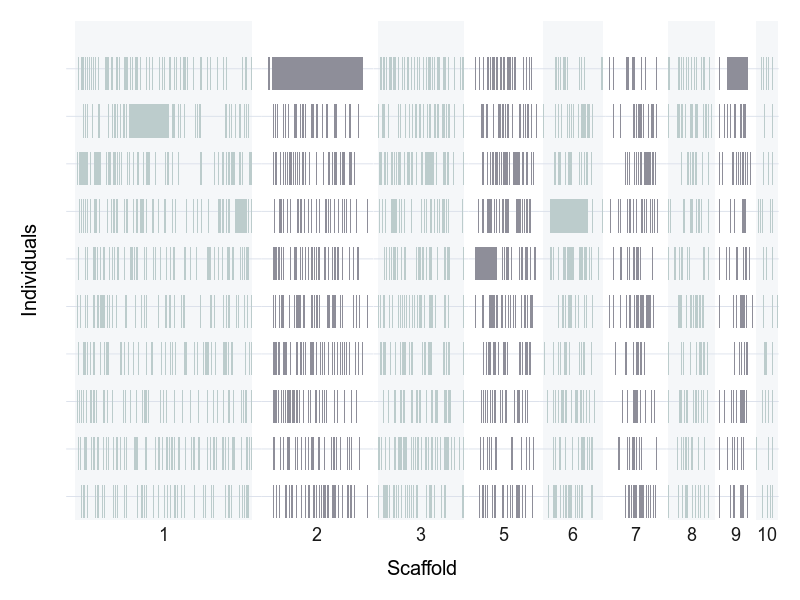
\includegraphics[keepaspectratio]{qmd/../plots/main/fig_1c.png}}

}

\caption{Detailed SnpEff annotation}

\end{figure}%

The mutations in the `high impact' category were used to calculate
individual genomic mutation load estimates.

\bookmarksetup{startatroot}

\chapter{GERP}\label{gerp}

\section{Introduction}\label{introduction-2}

\href{https://bio.tools/gerp}{GERP++} annotates a focal genome based on
evolutionary conserveration, where regions in the genome that show
higher conservation across multiple different species are expected to
face higher selective constraint. GERP score calculation, which indicate
the reduction in the number of substitutions compared to neutral
expectations, is done based on a multi-species alignment file. Higher
GERP scores indicate higher evolutionary constraint. First, we create
this MAF file using Progressive Cactus, then we calculate GERP scores
genome-wide, and select genomic positions with SNPs in our population.

\section{Methods}\label{methods-1}

\subsection{Creating the MAF}\label{creating-the-maf}

We use the publicly available 363 avian genomes
\href{https://cgl.gi.ucsc.edu/data/cactus/363-avian-2020.hal}{multi-alignment
file} as a starting point, and then reduce this file to exclude species
of the Neoaves clade. All the GERP analyses were done using the
\href{https://quay.io/repository/comparative-genomics-toolkit/cactus}{cactus
container}.

\begin{Shaded}
\begin{Highlighting}[]
\CommentTok{\#\#\# Remove subtrees that are not needed for ltet analysis}

\CommentTok{\#set cactus scratch directory}
\VariableTok{CACTUS\_SCRATCH}\OperatorTok{=}\VariableTok{$(}\BuiltInTok{pwd}\VariableTok{)}\NormalTok{/scratch/}

\CommentTok{\# enter the container}
\ExtensionTok{apptainer}\NormalTok{ shell }\AttributeTok{{-}{-}cleanenv} \DataTypeTok{\textbackslash{}}
  \AttributeTok{{-}{-}fakeroot} \AttributeTok{{-}{-}overlay} \VariableTok{$\{CACTUS\_SCRATCH\}} \DataTypeTok{\textbackslash{}}
  \AttributeTok{{-}{-}bind} \VariableTok{$\{CACTUS\_SCRATCH\}}\NormalTok{/tmp:/tmp,}\VariableTok{$(}\BuiltInTok{pwd}\VariableTok{)} \DataTypeTok{\textbackslash{}}
  \AttributeTok{{-}{-}env}\NormalTok{ PYTHONNOUSERSITE=1 }\DataTypeTok{\textbackslash{}}
\NormalTok{  docker:quay.io/comparative{-}genomics{-}toolkit/cactus:v2.5.1 }

\CommentTok{\# get stats on the original 363{-}avian multi{-}alignment file}
\ExtensionTok{halStats}\NormalTok{ data/genomic/intermediate/cactus/363{-}avian{-}2020.hal }\OperatorTok{\textgreater{}}\NormalTok{ output/cactus/stats\_original\_363\_hal.txt}

\CommentTok{\# copy the original file to then edit it}
\FunctionTok{cp}\NormalTok{ data/genomic/intermediate/cactus/363{-}avian{-}2020.hal data/genomic/intermediate/cactus/363{-}avian{-}reduced.hal}

\CommentTok{\# remove subtrees to exclude neoaves}
\ExtensionTok{halRemoveSubtree}\NormalTok{ data/genomic/intermediate/cactus/363{-}avian{-}reduced.hal birdAnc1}
\ExtensionTok{halRemoveSubtree}\NormalTok{ data/genomic/intermediate/cactus/363{-}avian{-}reduced.hal birdAnc57 }
\ExtensionTok{halRemoveSubtree}\NormalTok{ data/genomic/intermediate/cactus/363{-}avian{-}reduced.hal birdAnc69 }
\ExtensionTok{halRemoveSubtree}\NormalTok{ data/genomic/intermediate/cactus/363{-}avian{-}reduced.hal birdAnc318 }\CommentTok{\#starts with Heliornis\_fulica}
\ExtensionTok{halRemoveSubtree}\NormalTok{ data/genomic/intermediate/cactus/363{-}avian{-}reduced.hal birdAnc319 }\CommentTok{\#starts with Psophia\_crepitans}
\ExtensionTok{halRemoveSubtree}\NormalTok{ data/genomic/intermediate/cactus/363{-}avian{-}reduced.hal birdAnc320 }\CommentTok{\#starts with Charadrius\_vociferus}
\ExtensionTok{halRemoveSubtree}\NormalTok{ data/genomic/intermediate/cactus/363{-}avian{-}reduced.hal birdAnc321 }\CommentTok{\#starts with Opisthocomus\_hoazin}
\ExtensionTok{halRemoveSubtree}\NormalTok{ data/genomic/intermediate/cactus/363{-}avian{-}reduced.hal birdAnc322 }\CommentTok{\#stars with birdAnc57, so the big chunk of passerines but also a }

\CommentTok{\#some individual ancestral genomes left to exclude}
\ExtensionTok{halRemoveGenome}\NormalTok{ data/genomic/intermediate/cactus//363{-}avian{-}reduced.hal birdAnc322}
\ExtensionTok{halRemoveGenome}\NormalTok{ data/genomic/intermediate/cactus//363{-}avian{-}reduced.hal birdAnc1}

\CommentTok{\# get stats of our subset of genomes}

\ExtensionTok{halStats}\NormalTok{ data/genomic/intermediate/cactus/363{-}avian{-}reduced.hal }\OperatorTok{\textgreater{}}\NormalTok{ output/cactus/stats\_reduced\_363\_hal.txt}

\CommentTok{\#extract the reduced file }
\ExtensionTok{halExtract}\NormalTok{ data/genomic/intermediate/cactus/363{-}avian{-}reduced.hal data/genomic/intermediate/cactus/363{-}avian{-}reduced.hal }
\end{Highlighting}
\end{Shaded}

Next, we add two genomes: \emph{Lyrurus tetrix} and \emph{Lagopus
lecura}, using the \texttt{cactus\ prepare} function. To add the
\emph{Lagopus lecura} genome to the hal file, the assembly needs to be
downloaded from NCBI which can be found on NCBI:
https://0-www-ncbi-nlm-nih-gov.brum.beds.ac.uk/datasets/genome/GCF\_019238085.1/.

\begin{Shaded}
\begin{Highlighting}[]
\CommentTok{\# In this file, we will use the cactus{-}update{-}prepare function to create two scripts that will allow us to add two genomes to our dataset}

\CommentTok{\# set scratch directory}
\VariableTok{CACTUS\_SCRATCH}\OperatorTok{=}\VariableTok{$(}\BuiltInTok{pwd}\VariableTok{)}\NormalTok{/scratch/}

\CommentTok{\#enter container}
\ExtensionTok{apptainer}\NormalTok{ shell }\AttributeTok{{-}{-}cleanenv} \DataTypeTok{\textbackslash{}}
  \AttributeTok{{-}{-}fakeroot} \AttributeTok{{-}{-}overlay} \VariableTok{$\{CACTUS\_SCRATCH\}} \DataTypeTok{\textbackslash{}}
  \AttributeTok{{-}{-}bind} \VariableTok{$\{CACTUS\_SCRATCH\}}\NormalTok{/tmp:/tmp,}\VariableTok{$(}\BuiltInTok{pwd}\VariableTok{)} \DataTypeTok{\textbackslash{}}
  \AttributeTok{{-}{-}env}\NormalTok{ PYTHONNOUSERSITE=1 }\DataTypeTok{\textbackslash{}}
\NormalTok{  src/containers/cactus\_v2.5.1.sif }

\FunctionTok{sh}

\CommentTok{\#first add Lyrurus tetrix, branchlengths will be corrected in a later step}

\ExtensionTok{cactus{-}update{-}prepare} \DataTypeTok{\textbackslash{}}
\NormalTok{  add branch }\DataTypeTok{\textbackslash{}}
  \AttributeTok{{-}{-}parentGenome}\NormalTok{ birdAnc334 }\DataTypeTok{\textbackslash{}}
  \AttributeTok{{-}{-}childGenome}\NormalTok{ Tympanuchus\_cupido }\DataTypeTok{\textbackslash{}}
\NormalTok{  data/genomic/intermediate/cactus/363{-}avian{-}reduced.hal }\DataTypeTok{\textbackslash{}}
\NormalTok{  scripts/2\_cactus/input\_ltet.txt }\DataTypeTok{\textbackslash{}}
  \AttributeTok{{-}{-}cactus{-}prepare{-}options} \DataTypeTok{\textbackslash{}}
  \StringTok{\textquotesingle{}{-}{-}alignCores 4\textquotesingle{}} \DataTypeTok{\textbackslash{}}
  \AttributeTok{{-}{-}topBranchLength}\NormalTok{ 0.01 }\DataTypeTok{\textbackslash{} }
  \ExtensionTok{{-}{-}outDir}\NormalTok{ scratch/tmp/steps{-}output }\DataTypeTok{\textbackslash{}}
  \AttributeTok{{-}{-}jobStore}\NormalTok{ scratch/tmp/js }\DataTypeTok{\textbackslash{}}
  \AttributeTok{{-}{-}ancestorName}\NormalTok{ AncX }\OperatorTok{\textgreater{}}\NormalTok{ scripts/2\_cactus/3\_cactus\_update\_lyrurus\_steps.sh }

\CommentTok{\# then add Lagopus leucura}

\ExtensionTok{cactus{-}update{-}prepare} \DataTypeTok{\textbackslash{}}
\NormalTok{  add branch }\DataTypeTok{\textbackslash{}}
  \AttributeTok{{-}{-}parentGenome}\NormalTok{ AncX }\DataTypeTok{\textbackslash{}}
  \AttributeTok{{-}{-}childGenome}\NormalTok{ Lyrurus\_tetrix }\DataTypeTok{\textbackslash{}}
\NormalTok{  data/genomic/intermediate/cactus/363{-}avian{-}reduced.hal }\DataTypeTok{\textbackslash{}}
\NormalTok{  scripts/2\_cactus/input\_lleu.txt }\DataTypeTok{\textbackslash{}}
  \AttributeTok{{-}{-}cactus{-}prepare{-}options} \DataTypeTok{\textbackslash{}}
  \StringTok{\textquotesingle{}{-}{-}alignCores 4\textquotesingle{}} \DataTypeTok{\textbackslash{}}
  \AttributeTok{{-}{-}topBranchLength}\NormalTok{ 0.01 }\DataTypeTok{\textbackslash{}}
  \AttributeTok{{-}{-}outDir}\NormalTok{ scratch/tmp/steps{-}output }\DataTypeTok{\textbackslash{}}
  \AttributeTok{{-}{-}jobStore}\NormalTok{ scratch/tmp/js }\DataTypeTok{\textbackslash{}}
  \AttributeTok{{-}{-}ancestorName}\NormalTok{ AncY }\OperatorTok{\textgreater{}}\NormalTok{ scripts/2\_cactus/4\_cactus\_update\_lagopus\_steps.sh }
  
\end{Highlighting}
\end{Shaded}

This is just the preparation step, and two files will be outputted that
can be used to update the .hal file. This is what these files look like
(and then they have to be executed).

\begin{Shaded}
\begin{Highlighting}[]
\CommentTok{\#\# Preprocessor}
\ExtensionTok{cactus{-}preprocess}\NormalTok{ scratch/tmp/js/0 scratch/tmp/steps{-}output/seq\_file.in scratch/tmp/steps{-}output/seq\_file.out }\AttributeTok{{-}{-}inputNames}\NormalTok{ Lyrurus\_tetrix }\AttributeTok{{-}{-}realTimeLogging} \AttributeTok{{-}{-}logInfo} \AttributeTok{{-}{-}retryCount}\NormalTok{ 0 }\AttributeTok{{-}{-}maskMode}\NormalTok{ none}

\CommentTok{\#\# Alignment}

\CommentTok{\#\#\# Round 0}
\ExtensionTok{cactus{-}blast}\NormalTok{ scratch/tmp/js/1 scratch/tmp/steps{-}output/seq\_file.out scratch/tmp/steps{-}output/AncX.cigar }\AttributeTok{{-}{-}root}\NormalTok{ AncX }\AttributeTok{{-}{-}restart} 
\ExtensionTok{cactus{-}align}\NormalTok{ scratch/tmp/js/2 scratch/tmp/steps{-}output/seq\_file.out scratch/tmp/steps{-}output/AncX.cigar scratch/tmp/steps{-}output/AncX.hal }\AttributeTok{{-}{-}root}\NormalTok{ AncX  }\AttributeTok{{-}{-}maxCores}\NormalTok{ 8 }
\ExtensionTok{hal2fasta}\NormalTok{ scratch/tmp/steps{-}output/AncX.hal AncX }\AttributeTok{{-}{-}hdf5InMemory} \OperatorTok{\textgreater{}}\NormalTok{ scratch/tmp/steps{-}output/AncX.fa }

\CommentTok{\#\#\# Round 1}
\ExtensionTok{cactus{-}blast}\NormalTok{ scratch/tmp/js/3 scratch/tmp/steps{-}output/seq\_file.out scratch/tmp/steps{-}output/birdAnc334.cigar }\AttributeTok{{-}{-}root}\NormalTok{ birdAnc334 }\AttributeTok{{-}{-}includeRoot}  
\ExtensionTok{cactus{-}align}\NormalTok{ scratch/tmp/js/4 scratch/tmp/steps{-}output/seq\_file.out scratch/tmp/steps{-}output/birdAnc334.cigar scratch/tmp/steps{-}output/birdAnc334.hal }\AttributeTok{{-}{-}root}\NormalTok{ birdAnc334  }\AttributeTok{{-}{-}maxCores}\NormalTok{ 4 }\AttributeTok{{-}{-}includeRoot}  

\CommentTok{\#\# Alignment update}
\ExtensionTok{halAddToBranch}\NormalTok{ data/genomic/intermediate/cactus/363{-}avian{-}reduced.hal scratch/tmp/steps{-}output/AncX.hal scratch/tmp/steps{-}output/birdAnc334.hal birdAnc334 AncX Tympanuchus\_cupido Lyrurus\_tetrix 0.01 1.0 }\AttributeTok{{-}{-}hdf5InMemory} 

\CommentTok{\#\# Alignment validation}
\ExtensionTok{halValidate} \AttributeTok{{-}{-}genome}\NormalTok{ birdAnc334 data/genomic/intermediate/cactus/363{-}avian{-}reduced.hal }\AttributeTok{{-}{-}hdf5InMemory}
\ExtensionTok{halValidate} \AttributeTok{{-}{-}genome}\NormalTok{ AncX data/genomic/intermediate/cactus/363{-}avian{-}reduced.hal }\AttributeTok{{-}{-}hdf5InMemory}
\ExtensionTok{halValidate} \AttributeTok{{-}{-}genome}\NormalTok{ Tympanuchus\_cupido data/genomic/intermediate/cactus/363{-}avian{-}reduced.hal }\AttributeTok{{-}{-}hdf5InMemory}
\ExtensionTok{halValidate} \AttributeTok{{-}{-}genome}\NormalTok{ Lyrurus\_tetrix data/genomic/intermediate/cactus/363{-}avian{-}reduced.hal }\AttributeTok{{-}{-}hdf5InMemory}
\end{Highlighting}
\end{Shaded}

For subsequent steps, the resulting hal file is converted to maf format
per scaffold for both GERP++ and the neutral tree calculation. Note that
we only focus on the 30 largest scaffolds of the black grouse genome
which over \textgreater95\% of the genome, and only autosomal scaffolds.

This conversion is done within an R script

\begin{Shaded}
\begin{Highlighting}[]
\NormalTok{hal }\OtherTok{=}  \StringTok{"data/genomic/intermediate/cactus/363{-}avian{-}reduced.hal"}
\FunctionTok{library}\NormalTok{(dplyr); }\FunctionTok{library}\NormalTok{(data.table)}
\NormalTok{scafs }\OtherTok{\textless{}{-}} \FunctionTok{fread}\NormalTok{(}\StringTok{"data/genomic/refgenome/30\_largest.scafs.tsv"}\NormalTok{)}
\NormalTok{output\_dir }\OtherTok{=} \StringTok{"output/cactus/maf\_per\_scaf"}
\NormalTok{sif }\OtherTok{=} \StringTok{"src/containers/cactus\_v2.6.12.sif"}
\NormalTok{scratch }\OtherTok{=} \StringTok{"scripts/2\_cactus/scratch"}
\NormalTok{tmp\_js }\OtherTok{=} \StringTok{"scripts/2\_cactus/scratch/tmp/js/wiggle"}

\NormalTok{hal\_to\_maf\_per\_scaf }\OtherTok{\textless{}{-}} \ControlFlowTok{function}\NormalTok{(hal, scaf, outdir, scratch, i, sif, tmp\_js)\{}
    \FunctionTok{system}\NormalTok{(}\FunctionTok{paste0}\NormalTok{(}\StringTok{\textquotesingle{}/vol/apptainer/bin/apptainer run {-}{-}cleanenv {-}{-}fakeroot {-}{-}overlay \textquotesingle{}}\NormalTok{, scratch, }\StringTok{\textquotesingle{} {-}{-}bind \textquotesingle{}}\NormalTok{, scratch, }\StringTok{\textquotesingle{}/tmp:/tmp,\textquotesingle{}}\NormalTok{, scratch, }\StringTok{\textquotesingle{} {-}{-}env PYTHONNOUSERSITE=1 \textquotesingle{}}\NormalTok{, sif, }\StringTok{\textquotesingle{} cactus{-}hal2maf \textquotesingle{}}\NormalTok{, tmp\_js, }\StringTok{\textquotesingle{}/js\_\textquotesingle{}}\NormalTok{, i, }\StringTok{\textquotesingle{} {-}{-}restart \textquotesingle{}}\NormalTok{, hal, }\StringTok{\textquotesingle{} \textquotesingle{}}\NormalTok{, outdir, }\StringTok{\textquotesingle{}/maf\_\textquotesingle{}}\NormalTok{, i, }\StringTok{\textquotesingle{}.maf {-}{-}refGenome Lyrurus\_tetrix {-}{-}refSequence \textquotesingle{}}\NormalTok{, scaf, }\StringTok{\textquotesingle{} {-}{-}dupeMode single {-}{-}filterGapCausingDupes {-}{-}chunkSize 1000000 {-}{-}noAncestors\textquotesingle{}}\NormalTok{))}
\NormalTok{\}}

\ControlFlowTok{for}\NormalTok{ (i }\ControlFlowTok{in} \DecValTok{1}\SpecialCharTok{:}\DecValTok{30}\NormalTok{)\{}
  \FunctionTok{hal\_to\_maf\_per\_scaf}\NormalTok{(}\AttributeTok{hal =}\NormalTok{ hal,}
  \AttributeTok{scaf =}\NormalTok{ scafs}\SpecialCharTok{$}\NormalTok{scaf[i],}
  \AttributeTok{outdir =}\NormalTok{ output\_dir,}
  \AttributeTok{scratch =}\NormalTok{ scratch,}
  \AttributeTok{sif =}\NormalTok{ sif,}
  \AttributeTok{i =}\NormalTok{ i,}
  \AttributeTok{tmp\_js =}\NormalTok{ tmp\_js)}
\NormalTok{\}}
\end{Highlighting}
\end{Shaded}

Lastly, the final phylogenetic tree has to be recalculated according to
the updated tree, and the branch lengths have to be calculated in
substitutions/site (rather than million years ago). This analysis can be
found on github and will not be included here as it contains many small
steps integrated with in a snakemake workflow.

\subsection{Calculate GERP scores}\label{calculate-gerp-scores}

GERP scores were calculated per scaffold using snakemake using the
following rule:

\begin{Shaded}
\begin{Highlighting}[]
\ExtensionTok{rule}\NormalTok{ call\_gerp:}
    \ExtensionTok{input:}
      \ExtensionTok{maf}\NormalTok{ = }\StringTok{"output/cactus/maf\_per\_scaf/maf\_\{scaf\}.maf"}\NormalTok{,}
      \ExtensionTok{tree}\NormalTok{ = }\StringTok{"output/tree\_cactus\_updated.txt"}
    \ExtensionTok{output:}
      \ExtensionTok{rates}\NormalTok{ = }\StringTok{"output/gerp/maf\_\{scaf\}.maf.rates"}
    \ExtensionTok{params:}
      \ExtensionTok{refname}\NormalTok{ = }\StringTok{"Lyrurus\_tetrix"}
    \ExtensionTok{log:} \StringTok{"logs/gerp\_\{scaf\}.log"}
    \ExtensionTok{shell:}
      \StringTok{"""}
\StringTok{      gerpcol {-}t \{input.tree\} {-}f \{input.maf\} {-}e \{params.refname\} {-}j {-}z {-}x "}\ExtensionTok{.rates}\StringTok{" \&\textgreater{} \{log\}}
\StringTok{      """}
\end{Highlighting}
\end{Shaded}

\subsection{Overlap GERP scores with
SNPs}\label{overlap-gerp-scores-with-snps}

We are only interested in genomic locations where SNPs were found in our
population. Therefore, we convert our VCF file and GERP files to bed
format to overlap the SNPs with bedtools using the following commands
(integrated in snakemake):

\begin{Shaded}
\begin{Highlighting}[]
\ExtensionTok{rule}\NormalTok{ vcf\_to\_bed:}
    \ExtensionTok{input:}
        \ExtensionTok{vcf}\NormalTok{ = }\StringTok{"output/ancestral/ltet\_filtered\_ann\_aa.vcf.gz"}
    \ExtensionTok{output:}
        \ExtensionTok{bed}\NormalTok{ = }\StringTok{"output/ancestral/ltet\_filtered\_ann\_aa.bed"}
    \ExtensionTok{shell:}
        \StringTok{"""}
\StringTok{        convert2bed {-}i vcf \textless{} \{input.vcf\} \textgreater{} \{output.bed\}}

\StringTok{rule gerp\_to\_bed:}
\StringTok{    input:}
\StringTok{        rates = "}\ExtensionTok{output/gerp/maf\_per\_scaf/biggest\_30/maf\_\{nscaf\}.maf.rates}\StringTok{"}
\StringTok{    output:}
\StringTok{        bed = "}\ExtensionTok{output/gerp/beds/gerp\_scaf\_\{nscaf\}.bed}\StringTok{"}
\StringTok{    params:}
\StringTok{        outdir = "}\ExtensionTok{output/gerp/beds}\StringTok{"}
\StringTok{    log: "}\ExtensionTok{logs/gerp\_to\_bed\_\{nscaf\}}\StringTok{"}
\StringTok{    shell:}
\StringTok{        """}
        \ExtensionTok{Rscript} \AttributeTok{{-}{-}vanilla}\NormalTok{ scripts/6\_snpeff\_gerp/2\_gerp/gerp\_to\_bed.R \{input.rates\} \{output.bed\} \{params.outdir\} }\OperatorTok{\&\textgreater{}}\NormalTok{ \{log\}}
        \StringTok{"""}

\StringTok{rule bed\_overlap\_snps:}
\StringTok{    input:}
\StringTok{        bed = "}\ExtensionTok{output/gerp/beds/gerp\_scaf\_\{nscaf\}.bed}\StringTok{",}
\StringTok{        snps = "}\ExtensionTok{output/ancestral/ltet\_filtered\_ann\_aa.bed}\StringTok{"}
\StringTok{    output:}
\StringTok{        tsv = "}\ExtensionTok{output/gerp/beds/gerp\_overlapSNP\_scaf\_\{nscaf\}.tsv.gz}\StringTok{"}
\StringTok{    params:}
\StringTok{        tsv = "}\ExtensionTok{output/gerp/beds/gerp\_overlapSNP\_scaf\_\{nscaf\}.tsv}\StringTok{"    }
\StringTok{    shell:}
\StringTok{        """}
        \ExtensionTok{bedtools}\NormalTok{ intersect }\DataTypeTok{\textbackslash{}}
        \AttributeTok{{-}a}\NormalTok{ \{input.bed\} }\DataTypeTok{\textbackslash{}}
        \AttributeTok{{-}b}\NormalTok{ \{input.snps\} }\DataTypeTok{\textbackslash{}}
        \AttributeTok{{-}wa} \AttributeTok{{-}wb} \KeywordTok{|}
        \FunctionTok{cut} \AttributeTok{{-}f}\NormalTok{ 6{-}10 }\AttributeTok{{-}{-}complement} \OperatorTok{\textgreater{}}\NormalTok{ \{params.tsv\}}

        \FunctionTok{gzip}\NormalTok{ \{params.tsv\}}
        \StringTok{"""}
\end{Highlighting}
\end{Shaded}

As these files are still very large, we loop over scaffolds within
snakemake with an R script to count the number of mutations per
individual per scaffold, both in homozygosity and heterozygosity using
the following R formula (which is used for each scaffold separately and
outputs a tsv file used for calculating mutation load in the next
script).

\begin{Shaded}
\begin{Highlighting}[]
\NormalTok{calculate\_gerp\_load }\OtherTok{\textless{}{-}} \ControlFlowTok{function}\NormalTok{(gerp\_vcf, scafno)\{}
  \DocumentationTok{\#\# metadata on filenames and ids}
\NormalTok{  filenames }\OtherTok{\textless{}{-}} \FunctionTok{fread}\NormalTok{(}\StringTok{"data/genomic/raw/metadata/idnames.fam"}\NormalTok{)}
\NormalTok{  ids }\OtherTok{\textless{}{-}} \FunctionTok{fread}\NormalTok{(}\StringTok{"data/genomic/raw/metadata/file\_list\_all\_bgi\_clean.csv"}\NormalTok{)}
  
  \CommentTok{\#merge}
\NormalTok{  idnames }\OtherTok{\textless{}{-}} \FunctionTok{left\_join}\NormalTok{(filenames[,}\FunctionTok{c}\NormalTok{(}\StringTok{"V1"}\NormalTok{)], ids[,}\FunctionTok{c}\NormalTok{(}\StringTok{"loc"}\NormalTok{, }\StringTok{"id"}\NormalTok{)], }\AttributeTok{by =} \FunctionTok{c}\NormalTok{(}\StringTok{"V1"} \OtherTok{=} \StringTok{"loc"}\NormalTok{))}
  
\NormalTok{  file }\OtherTok{\textless{}{-}} \FunctionTok{read\_tsv}\NormalTok{(gerp\_vcf, }\AttributeTok{col\_names =} \FunctionTok{c}\NormalTok{(}\StringTok{"chr"}\NormalTok{, }\StringTok{"start"}\NormalTok{, }\StringTok{"pos"}\NormalTok{, }\StringTok{"neutral\_rate\_n"}\NormalTok{, }\StringTok{"rs\_score"}\NormalTok{, }\StringTok{"ancestral"}\NormalTok{, }\StringTok{"derived"}\NormalTok{, }\StringTok{"qual"}\NormalTok{, }\StringTok{"info"}\NormalTok{,}\StringTok{"format"}\NormalTok{, idnames}\SpecialCharTok{$}\NormalTok{id) )}\CommentTok{\#rename columns}
  
  \CommentTok{\# only get GT info, PL and DP are filtered by already anyway }
\NormalTok{  gt }\OtherTok{\textless{}{-}} \FunctionTok{c}\NormalTok{(}\DecValTok{11}\SpecialCharTok{:}\FunctionTok{ncol}\NormalTok{(file))}
\NormalTok{  select\_n3 }\OtherTok{\textless{}{-}} \ControlFlowTok{function}\NormalTok{(x)\{x }\OtherTok{=} \FunctionTok{substr}\NormalTok{(x,}\DecValTok{1}\NormalTok{,}\DecValTok{3}\NormalTok{)\}}
\NormalTok{  file[gt] }\OtherTok{\textless{}{-}} \FunctionTok{lapply}\NormalTok{(file[gt], select\_n3)}
  
  \CommentTok{\# replace genotype with RS value but separate per zygosity, do per ID}
\NormalTok{  gerp\_load }\OtherTok{\textless{}{-}} \FunctionTok{list}\NormalTok{()}
  \ControlFlowTok{for}\NormalTok{( id }\ControlFlowTok{in} \DecValTok{11}\SpecialCharTok{:}\FunctionTok{ncol}\NormalTok{(file))\{}
\NormalTok{    subset\_id }\OtherTok{\textless{}{-}}\NormalTok{ file[,}\FunctionTok{c}\NormalTok{(}\DecValTok{1}\SpecialCharTok{:}\DecValTok{10}\NormalTok{, id)]}
\NormalTok{    subset\_id }\OtherTok{\textless{}{-}}\NormalTok{ subset\_id }\SpecialCharTok{\%\textgreater{}\%} \FunctionTok{mutate}\NormalTok{(}\AttributeTok{gerp\_cat =} \FunctionTok{as.factor}\NormalTok{(}\FunctionTok{case\_when}\NormalTok{(}
\NormalTok{        rs\_score }\SpecialCharTok{\textless{}} \DecValTok{0} \SpecialCharTok{\textasciitilde{}} \StringTok{"\textless{} 0"}\NormalTok{, }\CommentTok{\#changed}
\NormalTok{        rs\_score }\SpecialCharTok{\textgreater{}=} \DecValTok{0} \SpecialCharTok{\&}\NormalTok{ rs\_score }\SpecialCharTok{\textless{}} \DecValTok{1} \SpecialCharTok{\textasciitilde{}} \StringTok{"0{-}1"}\NormalTok{,}
\NormalTok{        rs\_score }\SpecialCharTok{\textgreater{}=} \DecValTok{1} \SpecialCharTok{\&}\NormalTok{ rs\_score }\SpecialCharTok{\textless{}} \DecValTok{2} \SpecialCharTok{\textasciitilde{}} \StringTok{"1{-}2"}\NormalTok{,}
\NormalTok{        rs\_score }\SpecialCharTok{\textgreater{}=} \DecValTok{2} \SpecialCharTok{\&}\NormalTok{ rs\_score }\SpecialCharTok{\textless{}} \DecValTok{3} \SpecialCharTok{\textasciitilde{}} \StringTok{"2{-}3"}\NormalTok{,}
\NormalTok{        rs\_score }\SpecialCharTok{\textgreater{}=} \DecValTok{3} \SpecialCharTok{\&}\NormalTok{ rs\_score }\SpecialCharTok{\textless{}} \DecValTok{4} \SpecialCharTok{\textasciitilde{}} \StringTok{"3{-}4"}\NormalTok{,}
\NormalTok{        rs\_score }\SpecialCharTok{\textgreater{}=} \DecValTok{4} \SpecialCharTok{\textasciitilde{}} \StringTok{"4{-}5"}
\NormalTok{    )))}
\NormalTok{    gerp\_load\_id }\OtherTok{\textless{}{-}} \FunctionTok{list}\NormalTok{()}
    \ControlFlowTok{for}\NormalTok{ (i }\ControlFlowTok{in} \FunctionTok{c}\NormalTok{(}\StringTok{"\textless{} 0"}\NormalTok{, }\StringTok{"0{-}1"}\NormalTok{, }\StringTok{"1{-}2"}\NormalTok{, }\StringTok{"2{-}3"}\NormalTok{, }\StringTok{"3{-}4"}\NormalTok{, }\StringTok{"4{-}5"}\NormalTok{))\{}\CommentTok{\#changed}
\NormalTok{        cat\_subset }\OtherTok{\textless{}{-}} \FunctionTok{subset}\NormalTok{(subset\_id, gerp\_cat }\SpecialCharTok{==}\NormalTok{ i)}
\NormalTok{        het\_data }\OtherTok{\textless{}{-}} \FunctionTok{subset}\NormalTok{(cat\_subset, cat\_subset[[}\DecValTok{11}\NormalTok{]] }\SpecialCharTok{==} \StringTok{"1/0"} \SpecialCharTok{|}\NormalTok{ cat\_subset[[}\DecValTok{11}\NormalTok{]] }\SpecialCharTok{==} \StringTok{"0/1"}\NormalTok{)}
\NormalTok{        hom\_data }\OtherTok{\textless{}{-}} \FunctionTok{subset}\NormalTok{(cat\_subset, cat\_subset[[}\DecValTok{11}\NormalTok{]] }\SpecialCharTok{==} \StringTok{"1/1"}\NormalTok{)}
\NormalTok{        n\_genotyped }\OtherTok{\textless{}{-}} \FunctionTok{nrow}\NormalTok{(cat\_subset) }\SpecialCharTok{{-}} \FunctionTok{nrow}\NormalTok{(}\FunctionTok{subset}\NormalTok{(cat\_subset, cat\_subset[[}\DecValTok{11}\NormalTok{]] }\SpecialCharTok{==} \StringTok{"./."}\NormalTok{))}
\NormalTok{        n\_total }\OtherTok{\textless{}{-}} \FunctionTok{nrow}\NormalTok{(cat\_subset)}
\NormalTok{        df }\OtherTok{\textless{}{-}} \FunctionTok{data.frame}\NormalTok{(}\AttributeTok{id =} \FunctionTok{colnames}\NormalTok{(file[id]),}
                         \AttributeTok{gerp\_cat =}\NormalTok{ i,}
                         \AttributeTok{scafno =}\NormalTok{ scafno,}
                         \AttributeTok{n\_total =}\NormalTok{ n\_total,}
                         \AttributeTok{n\_genotyped =}\NormalTok{ n\_genotyped,}
                         \AttributeTok{het\_data =} \FunctionTok{nrow}\NormalTok{(het\_data),}
                         \AttributeTok{hom\_data =} \FunctionTok{nrow}\NormalTok{(hom\_data))}
        
\NormalTok{        gerp\_load\_id[[i]] }\OtherTok{\textless{}{-}}\NormalTok{ df}
        
\NormalTok{        \}}
\NormalTok{        gerp\_load\_id }\OtherTok{\textless{}{-}} \FunctionTok{do.call}\NormalTok{(rbind.data.frame, gerp\_load\_id)}
        \FunctionTok{rownames}\NormalTok{(gerp\_load\_id) }\OtherTok{\textless{}{-}} \ConstantTok{NULL}
    
\NormalTok{    gerp\_load[[id]] }\OtherTok{\textless{}{-}}\NormalTok{ gerp\_load\_id}
\NormalTok{    \}}
\NormalTok{  gerp\_load }\OtherTok{\textless{}{-}} \FunctionTok{do.call}\NormalTok{(rbind.data.frame, gerp\_load)}

    \FunctionTok{return}\NormalTok{(gerp\_load)\}}
\end{Highlighting}
\end{Shaded}

\section{Results}\label{results-1}

We identified 413,489 mutations with a GERP score higher than or equal
to 4:
\pandocbounded{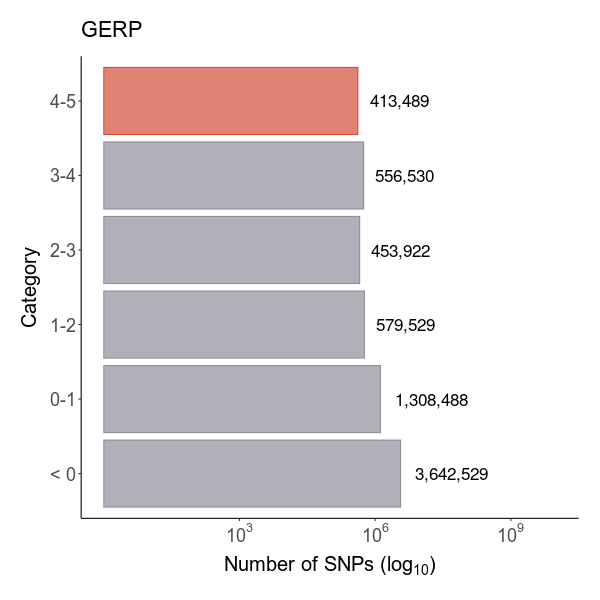
\includegraphics[keepaspectratio]{qmd/../plots/main/fig_1a.png}}

These mutations were used to calculate mutation load in the next script.

\bookmarksetup{startatroot}

\chapter{Calculating mutation load}\label{calculating-mutation-load}

\section{Introduction}\label{introduction-3}

There are various types of load and in general, mutation load can be
divided between potential and realized load. Realized load (also known
as expressed load) only includes the deleterious mutations that are
expressed in the individual \autocite{bertorelleGeneticLoadGenomic2022}.
Potential load (also known as inbreeding or masked load) is the fitness
reduction due to deleterious mutations, of which not all are expressed
on an individual level and therefore quantifies recessive deleterious
mutations that could be expressed in future generations
\autocite{bertorelleGeneticLoadGenomic2022}.

However, to be able to distinguish between realized and potential load,
you need to know dominance coefficients, which we do not. Therefore, we
focus on homozygous and heterozygous load instead, which consists of
mutations in homo- and heterozygosity in an individual instead. The
total load sums the number of mutations contributing to the load, where
heterozygous mutations are counted ones (one per allele) and homozygous
mutations twice (one per allele).

From here on onwards, the majority of analyses are computed within R
(instead of bash scripts/snakemake).

\section{Mutation load (SnpEff)}\label{mutation-load-snpeff}

Here, we load in the .vcf file outputted by SnpSift with only high
impact SnpEff mutations, add column names, include only the 29 largest
autosomal scaffolds, exclude warning messages, convert the genotype
columns into only 1/1, 1/0, 0/1, 0/0 and ./. values, calculate load per
individual, and then merge the load estimates of all individuals
together.

\begin{Shaded}
\begin{Highlighting}[]
\DocumentationTok{\#\#\# load packages }\AlertTok{\#\#\#}
\NormalTok{pacman}\SpecialCharTok{::}\FunctionTok{p\_load}\NormalTok{(dplyr, data.table)}

\DocumentationTok{\#\#\# function to calculate load }\AlertTok{\#\#\#}
\NormalTok{calculate\_load\_snpeff }\OtherTok{\textless{}{-}} \ControlFlowTok{function}\NormalTok{(vcf, output\_vcf, loadtype)\{}
  \DocumentationTok{\#\# metadata on filenames and ids}
\NormalTok{  filenames }\OtherTok{\textless{}{-}} \FunctionTok{fread}\NormalTok{(}\StringTok{"data/genomic/raw/metadata/idnames.fam"}\NormalTok{)}
\NormalTok{  ids }\OtherTok{\textless{}{-}} \FunctionTok{fread}\NormalTok{(}\StringTok{"data/genomic/raw/metadata/file\_list\_all\_bgi\_clean.csv"}\NormalTok{)}
  
  \CommentTok{\#merge}
\NormalTok{  idnames }\OtherTok{\textless{}{-}} \FunctionTok{left\_join}\NormalTok{(filenames[,}\FunctionTok{c}\NormalTok{(}\StringTok{"V1"}\NormalTok{)], ids[,}\FunctionTok{c}\NormalTok{(}\StringTok{"loc"}\NormalTok{, }\StringTok{"id"}\NormalTok{)], }\AttributeTok{by =} \FunctionTok{c}\NormalTok{(}\StringTok{"V1"} \OtherTok{=} \StringTok{"loc"}\NormalTok{))}
  
  \FunctionTok{names}\NormalTok{(vcf) }\OtherTok{\textless{}{-}} \FunctionTok{c}\NormalTok{(}\FunctionTok{c}\NormalTok{(}\StringTok{"CHROM"}\NormalTok{, }\StringTok{"POS"}\NormalTok{, }\StringTok{"ID"}\NormalTok{, }\StringTok{"REF"}\NormalTok{, }\StringTok{"ALT"}\NormalTok{, }\StringTok{"QUAL"}\NormalTok{, }\StringTok{"FILTER"}\NormalTok{, }\StringTok{"INFO"}\NormalTok{,}\StringTok{"FORMAT"}\NormalTok{), idnames}\SpecialCharTok{$}\NormalTok{id)}\CommentTok{\#rename columns}

  \CommentTok{\# only select 29 largest autosomal scaffolds}
\NormalTok{  scaf }\OtherTok{\textless{}{-}} \FunctionTok{fread}\NormalTok{(}\StringTok{"data/genomic/refgenome/30\_largest.scafs.tsv"}\NormalTok{)}
\NormalTok{  scaf}\SpecialCharTok{$}\NormalTok{scaf }\OtherTok{\textless{}{-}} \FunctionTok{gsub}\NormalTok{(}\StringTok{":"}\NormalTok{, }\StringTok{";"}\NormalTok{, scaf}\SpecialCharTok{$}\NormalTok{scaf)}
\NormalTok{  scaf}\SpecialCharTok{$}\NormalTok{scaf }\OtherTok{\textless{}{-}} \FunctionTok{gsub}\NormalTok{(}\StringTok{"}\SpecialCharTok{\textbackslash{}\textbackslash{}}\StringTok{."}\NormalTok{, }\StringTok{"="}\NormalTok{, scaf}\SpecialCharTok{$}\NormalTok{scaf)}
\NormalTok{  scaf }\OtherTok{\textless{}{-}} \FunctionTok{subset}\NormalTok{(scaf, scaf\_no }\SpecialCharTok{!=} \DecValTok{4}\NormalTok{)}
  
\NormalTok{  vcf }\OtherTok{\textless{}{-}} \FunctionTok{subset}\NormalTok{(vcf, CHROM }\SpecialCharTok{\%in\%}\NormalTok{ scaf}\SpecialCharTok{$}\NormalTok{scaf)}
  
  \CommentTok{\# exclude warning messages}
  
\NormalTok{  vcf }\OtherTok{\textless{}{-}} \FunctionTok{subset}\NormalTok{(vcf, }\SpecialCharTok{!}\FunctionTok{grepl}\NormalTok{(}\StringTok{"WARNING"}\NormalTok{, INFO))}
  
  \CommentTok{\# only get GT info, PL and DP are filtered by already anyway }
\NormalTok{  gt }\OtherTok{\textless{}{-}} \FunctionTok{c}\NormalTok{(}\DecValTok{10}\SpecialCharTok{:}\FunctionTok{ncol}\NormalTok{(vcf))}
\NormalTok{  select\_n3 }\OtherTok{\textless{}{-}} \ControlFlowTok{function}\NormalTok{(x)\{x }\OtherTok{=} \FunctionTok{substr}\NormalTok{(x,}\DecValTok{1}\NormalTok{,}\DecValTok{3}\NormalTok{)\}}
\NormalTok{  vcf[gt] }\OtherTok{\textless{}{-}} \FunctionTok{lapply}\NormalTok{(vcf[gt], select\_n3)}
  
  \CommentTok{\# calculate load}
\NormalTok{  load }\OtherTok{\textless{}{-}} \FunctionTok{list}\NormalTok{()}
  \CommentTok{\# loop over ids}
  \ControlFlowTok{for}\NormalTok{( id }\ControlFlowTok{in} \DecValTok{10}\SpecialCharTok{:}\NormalTok{(}\FunctionTok{ncol}\NormalTok{(vcf)))\{}
    \CommentTok{\# subset per id}
\NormalTok{    subset\_id }\OtherTok{\textless{}{-}}\NormalTok{ vcf[,}\FunctionTok{c}\NormalTok{(}\DecValTok{1}\SpecialCharTok{:}\DecValTok{9}\NormalTok{, id)]}
    
    \CommentTok{\# filter for snps in het and hom}
\NormalTok{    het\_data }\OtherTok{\textless{}{-}} \FunctionTok{subset}\NormalTok{(subset\_id, subset\_id[[}\DecValTok{10}\NormalTok{]] }\SpecialCharTok{==} \StringTok{"1/0"} \SpecialCharTok{|}\NormalTok{ subset\_id[[}\DecValTok{10}\NormalTok{]] }\SpecialCharTok{==} \StringTok{"0/1"}\NormalTok{)}
\NormalTok{    hom\_data }\OtherTok{\textless{}{-}} \FunctionTok{subset}\NormalTok{(subset\_id, subset\_id[[}\DecValTok{10}\NormalTok{]] }\SpecialCharTok{==} \StringTok{"1/1"}\NormalTok{)}
    
    \CommentTok{\# count amount of snps in het and hom}
\NormalTok{    het\_load\_sum }\OtherTok{\textless{}{-}} \FunctionTok{nrow}\NormalTok{(het\_data)}
\NormalTok{    hom\_load\_sum }\OtherTok{\textless{}{-}} \FunctionTok{nrow}\NormalTok{(hom\_data)}
    
    \CommentTok{\# count no of snps successfully genotyped}
\NormalTok{    n\_genotyped }\OtherTok{\textless{}{-}} \FunctionTok{nrow}\NormalTok{(subset\_id) }\SpecialCharTok{{-}} \FunctionTok{nrow}\NormalTok{(}\FunctionTok{subset}\NormalTok{(subset\_id, subset\_id[[}\DecValTok{10}\NormalTok{]] }\SpecialCharTok{==} \StringTok{"./."}\NormalTok{))}
\NormalTok{    n\_total }\OtherTok{\textless{}{-}} \FunctionTok{nrow}\NormalTok{(subset\_id)}
    
    \CommentTok{\# collect data in df}
\NormalTok{    df }\OtherTok{\textless{}{-}} \FunctionTok{data.frame}\NormalTok{(}\AttributeTok{id =} \FunctionTok{colnames}\NormalTok{(vcf[id]),}
                     \AttributeTok{n\_total =}\NormalTok{ n\_total,}
                     \AttributeTok{n\_genotyped =}\NormalTok{ n\_genotyped,}
                     \AttributeTok{het\_load =}\NormalTok{ het\_load\_sum }\SpecialCharTok{/}\NormalTok{ n\_genotyped,}
                     \AttributeTok{hom\_load =}\NormalTok{ hom\_load\_sum }\SpecialCharTok{/}\NormalTok{ n\_genotyped,}
                     \AttributeTok{total\_load =}\NormalTok{ (het\_load\_sum}\SpecialCharTok{*}\FloatTok{0.5} \SpecialCharTok{+}\NormalTok{ hom\_load\_sum) }\SpecialCharTok{/}\NormalTok{ n\_genotyped,}
                     \AttributeTok{loadtype =}\NormalTok{ loadtype)}
\NormalTok{    load[[id]] }\OtherTok{\textless{}{-}}\NormalTok{ df}
\NormalTok{  \}}
  \CommentTok{\# convert list to df}
\NormalTok{  load }\OtherTok{\textless{}{-}} \FunctionTok{do.call}\NormalTok{(rbind.data.frame, load)}
  
  \ControlFlowTok{if}\NormalTok{(output\_vcf }\SpecialCharTok{==} \ConstantTok{TRUE}\NormalTok{)\{}
\NormalTok{    out }\OtherTok{\textless{}{-}} \FunctionTok{list}\NormalTok{(}\AttributeTok{load =}\NormalTok{ load, }\AttributeTok{vcf =}\NormalTok{ vcf)}
    \FunctionTok{return}\NormalTok{(out)}
\NormalTok{  \}}
  
  \ControlFlowTok{if}\NormalTok{(output\_vcf}\SpecialCharTok{==}\ConstantTok{FALSE}\NormalTok{)\{}
    \FunctionTok{return}\NormalTok{(load)\}}
\NormalTok{\}}

\DocumentationTok{\#\#\#\#\# load high impact mutations (filtered by snpsift) \#\#\#\#\#}

\NormalTok{high }\OtherTok{\textless{}{-}} \FunctionTok{read.table}\NormalTok{(}\StringTok{"data/genomic/intermediate/snpef/ltet\_ann\_aa\_snp\_output\_HIGH.vcf.gz"}\NormalTok{)}

\DocumentationTok{\#\# calculate load }
\CommentTok{\# in this function, we give the columns names, filter for only the largest 29 autosomal scaffolds and exclude annotations with warning messages}

\NormalTok{high\_load }\OtherTok{\textless{}{-}} \FunctionTok{calculate\_load\_snpeff}\NormalTok{(high, }\AttributeTok{output\_vcf =} \ConstantTok{TRUE}\NormalTok{, }\AttributeTok{loadtype =} \StringTok{"high"}\NormalTok{)}
\end{Highlighting}
\end{Shaded}

\section{Mutation load (GERP)}\label{mutation-load-gerp}

Here, we load in the .bed files that contain GERP scores from SNPs,
filter for those with GERP values \textgreater= 4, add column names,
convert the genotype columns into only 1/1, 1/0, 0/1, 0/0 and ./.
values, calculate load per individual, and then merge the load estimates
of all individuals together. Note this step is quite time-intensive as
the .bed files are large in filesize!

\begin{Shaded}
\begin{Highlighting}[]
\CommentTok{\# load in all bed files with gerp scores that overlap a SNP}
\NormalTok{gerp\_snp\_scafs }\OtherTok{\textless{}{-}} \FunctionTok{list.files}\NormalTok{(}\AttributeTok{path =} \StringTok{"output/gerp/beds"}\NormalTok{, }\AttributeTok{pattern =} \StringTok{"gerp\_overlapSNP*"}\NormalTok{, }\AttributeTok{full.names =}\NormalTok{ T)}
\NormalTok{gerp\_snp\_scafs }\OtherTok{\textless{}{-}}\NormalTok{ gerp\_snp\_scafs[}\SpecialCharTok{{-}}\DecValTok{22}\NormalTok{] }\CommentTok{\#empty, scaffold 29 has no SNPs with gerp scores}

\NormalTok{gerp\_snp }\OtherTok{\textless{}{-}} \FunctionTok{data.frame}\NormalTok{()}
\ControlFlowTok{for}\NormalTok{ (i }\ControlFlowTok{in} \DecValTok{1}\SpecialCharTok{:}\FunctionTok{length}\NormalTok{(gerp\_snp\_scafs))\{}
\NormalTok{  scaf }\OtherTok{\textless{}{-}} \FunctionTok{read.table}\NormalTok{(gerp\_snp\_scafs[i])}
\NormalTok{  scaf }\OtherTok{\textless{}{-}}\NormalTok{ scaf }\SpecialCharTok{\%\textgreater{}\%} \FunctionTok{filter}\NormalTok{(V5 }\SpecialCharTok{\textgreater{}=} \DecValTok{4}\NormalTok{)}
\NormalTok{  gerp\_snp }\OtherTok{\textless{}{-}} \FunctionTok{rbind}\NormalTok{(gerp\_snp, scaf)}
\NormalTok{\}}

\DocumentationTok{\#\# function to calculate load}

\NormalTok{calculate\_load\_gerp }\OtherTok{\textless{}{-}} \ControlFlowTok{function}\NormalTok{(vcf, output\_vcf, loadtype)\{}
  
  \DocumentationTok{\#\# metadata on filenames and ids}
\NormalTok{  filenames }\OtherTok{\textless{}{-}} \FunctionTok{fread}\NormalTok{(}\StringTok{"data/genomic/raw/metadata/idnames.fam"}\NormalTok{)}
\NormalTok{  ids }\OtherTok{\textless{}{-}} \FunctionTok{fread}\NormalTok{(}\StringTok{"data/genomic/raw/metadata/file\_list\_all\_bgi\_clean.csv"}\NormalTok{)}
  
  \CommentTok{\#merge}
\NormalTok{  idnames }\OtherTok{\textless{}{-}} \FunctionTok{left\_join}\NormalTok{(filenames[,}\FunctionTok{c}\NormalTok{(}\StringTok{"V1"}\NormalTok{)], ids[,}\FunctionTok{c}\NormalTok{(}\StringTok{"loc"}\NormalTok{, }\StringTok{"id"}\NormalTok{)], }\AttributeTok{by =} \FunctionTok{c}\NormalTok{(}\StringTok{"V1"} \OtherTok{=} \StringTok{"loc"}\NormalTok{))}
  
  \FunctionTok{names}\NormalTok{(vcf) }\OtherTok{\textless{}{-}} \FunctionTok{c}\NormalTok{(}\StringTok{"chr"}\NormalTok{, }\StringTok{"start"}\NormalTok{, }\StringTok{"pos"}\NormalTok{, }\StringTok{"neutral\_rate\_n"}\NormalTok{, }\StringTok{"rs\_score"}\NormalTok{, }\StringTok{"ancestral"}\NormalTok{, }\StringTok{"derived"}\NormalTok{, }\StringTok{"qual"}\NormalTok{, }\StringTok{"info"}\NormalTok{,}\StringTok{"format"}\NormalTok{, idnames}\SpecialCharTok{$}\NormalTok{id) }\CommentTok{\#rename columns}
  
  \CommentTok{\# only get GT info, PL and DP are filtered by already anyway }
\NormalTok{  gt }\OtherTok{\textless{}{-}} \FunctionTok{c}\NormalTok{(}\DecValTok{11}\SpecialCharTok{:}\FunctionTok{ncol}\NormalTok{(vcf))}
\NormalTok{  select\_n3 }\OtherTok{\textless{}{-}} \ControlFlowTok{function}\NormalTok{(x)\{x }\OtherTok{=} \FunctionTok{substr}\NormalTok{(x,}\DecValTok{1}\NormalTok{,}\DecValTok{3}\NormalTok{)\}}
\NormalTok{  vcf[gt] }\OtherTok{\textless{}{-}} \FunctionTok{lapply}\NormalTok{(vcf[gt], select\_n3)}
  
  \CommentTok{\# calculate load}
\NormalTok{  load }\OtherTok{\textless{}{-}} \FunctionTok{list}\NormalTok{()}
  \CommentTok{\# loop over ids}
  \ControlFlowTok{for}\NormalTok{( id }\ControlFlowTok{in} \DecValTok{11}\SpecialCharTok{:}\NormalTok{(}\FunctionTok{ncol}\NormalTok{(vcf)))\{}
    \CommentTok{\# subset per id}
\NormalTok{    subset\_id }\OtherTok{\textless{}{-}}\NormalTok{ vcf[,}\FunctionTok{c}\NormalTok{(}\DecValTok{1}\SpecialCharTok{:}\DecValTok{10}\NormalTok{, id)]}
    
    \CommentTok{\# filter for snps in het and hom}
\NormalTok{    het\_data }\OtherTok{\textless{}{-}} \FunctionTok{subset}\NormalTok{(subset\_id, subset\_id[[}\DecValTok{11}\NormalTok{]] }\SpecialCharTok{==} \StringTok{"1/0"} \SpecialCharTok{|}\NormalTok{ subset\_id[[}\DecValTok{11}\NormalTok{]] }\SpecialCharTok{==} \StringTok{"0/1"}\NormalTok{)}
\NormalTok{    hom\_data }\OtherTok{\textless{}{-}} \FunctionTok{subset}\NormalTok{(subset\_id, subset\_id[[}\DecValTok{11}\NormalTok{]] }\SpecialCharTok{==} \StringTok{"1/1"}\NormalTok{)}
    
    \CommentTok{\# count amount of snps in het and hom}
\NormalTok{    het\_load\_sum }\OtherTok{\textless{}{-}} \FunctionTok{nrow}\NormalTok{(het\_data)}
\NormalTok{    hom\_load\_sum }\OtherTok{\textless{}{-}} \FunctionTok{nrow}\NormalTok{(hom\_data)}
    
    \CommentTok{\# count no of snps successfully genotyped}
\NormalTok{    n\_genotyped }\OtherTok{\textless{}{-}} \FunctionTok{nrow}\NormalTok{(subset\_id) }\SpecialCharTok{{-}} \FunctionTok{nrow}\NormalTok{(}\FunctionTok{subset}\NormalTok{(subset\_id, subset\_id[[}\DecValTok{11}\NormalTok{]] }\SpecialCharTok{==} \StringTok{"./."}\NormalTok{))}
\NormalTok{    n\_total }\OtherTok{\textless{}{-}} \FunctionTok{nrow}\NormalTok{(subset\_id)}
    
    \CommentTok{\# collect data in df}
\NormalTok{    df }\OtherTok{\textless{}{-}} \FunctionTok{data.frame}\NormalTok{(}\AttributeTok{id =} \FunctionTok{colnames}\NormalTok{(vcf[id]),}
                     \AttributeTok{n\_total =}\NormalTok{ n\_total,}
                     \AttributeTok{n\_genotyped =}\NormalTok{ n\_genotyped,}
                     \AttributeTok{het\_load =}\NormalTok{ het\_load\_sum }\SpecialCharTok{/}\NormalTok{ n\_genotyped,}
                     \AttributeTok{hom\_load =}\NormalTok{ hom\_load\_sum }\SpecialCharTok{/}\NormalTok{ n\_genotyped,}
                     \AttributeTok{total\_load =}\NormalTok{ (het\_load\_sum}\SpecialCharTok{*}\FloatTok{0.5} \SpecialCharTok{+}\NormalTok{ hom\_load\_sum) }\SpecialCharTok{/}\NormalTok{ n\_genotyped,}
                     \AttributeTok{loadtype =}\NormalTok{ loadtype)}
\NormalTok{    load[[id]] }\OtherTok{\textless{}{-}}\NormalTok{ df}
\NormalTok{  \}}
  \CommentTok{\# convert list to df}
\NormalTok{  load }\OtherTok{\textless{}{-}} \FunctionTok{do.call}\NormalTok{(rbind.data.frame, load)}
  
  \ControlFlowTok{if}\NormalTok{(output\_vcf }\SpecialCharTok{==} \ConstantTok{TRUE}\NormalTok{)\{}
\NormalTok{    out }\OtherTok{\textless{}{-}} \FunctionTok{list}\NormalTok{(}\AttributeTok{load =}\NormalTok{ load, }\AttributeTok{vcf =}\NormalTok{ vcf)}
    \FunctionTok{return}\NormalTok{(out)}
\NormalTok{  \}}
  
  \ControlFlowTok{if}\NormalTok{(output\_vcf}\SpecialCharTok{==}\ConstantTok{FALSE}\NormalTok{)\{}
  \FunctionTok{return}\NormalTok{(load)\}}
\NormalTok{\}}

\DocumentationTok{\#\# calculate load}
\NormalTok{gerp\_45 }\OtherTok{\textless{}{-}} \FunctionTok{calculate\_load\_gerp}\NormalTok{(gerp\_snp, }\AttributeTok{output\_vcf =} \ConstantTok{TRUE}\NormalTok{, }\AttributeTok{loadtype =} \StringTok{"gerp45"}\NormalTok{) }
\NormalTok{gerp }\OtherTok{\textless{}{-}}\NormalTok{ gerp\_45\_load\_check}\SpecialCharTok{$}\NormalTok{vcf}
\end{Highlighting}
\end{Shaded}

\subsection{Combine loads}\label{combine-loads}

Note: the analyses done above was also done for other mutation
categories, e.g.~low and moderate impact classes and GERP scores between
3-4. All load scores are then combined into a single file:

\begin{Shaded}
\begin{Highlighting}[]
\NormalTok{load }\OtherTok{\textless{}{-}} \FunctionTok{rbind}\NormalTok{(high\_load}\SpecialCharTok{$}\NormalTok{load[,}\FunctionTok{c}\NormalTok{(}\StringTok{"id"}\NormalTok{, }\StringTok{"het\_load"}\NormalTok{, }\StringTok{"hom\_load"}\NormalTok{, }\StringTok{"total\_load"}\NormalTok{, }\StringTok{"loadtype"}\NormalTok{)] ,}
\NormalTok{              moderate\_load[,}\FunctionTok{c}\NormalTok{(}\StringTok{"id"}\NormalTok{, }\StringTok{"het\_load"}\NormalTok{, }\StringTok{"hom\_load"}\NormalTok{, }\StringTok{"total\_load"}\NormalTok{, }\StringTok{"loadtype"}\NormalTok{)], }
\NormalTok{              low\_load[,}\FunctionTok{c}\NormalTok{(}\StringTok{"id"}\NormalTok{, }\StringTok{"het\_load"}\NormalTok{, }\StringTok{"hom\_load"}\NormalTok{, }\StringTok{"total\_load"}\NormalTok{, }\StringTok{"loadtype"}\NormalTok{)],}
\NormalTok{              lof\_load[,}\FunctionTok{c}\NormalTok{(}\StringTok{"id"}\NormalTok{, }\StringTok{"het\_load"}\NormalTok{, }\StringTok{"hom\_load"}\NormalTok{, }\StringTok{"total\_load"}\NormalTok{, }\StringTok{"loadtype"}\NormalTok{)],}
\NormalTok{              missense\_load[,}\FunctionTok{c}\NormalTok{(}\StringTok{"id"}\NormalTok{, }\StringTok{"het\_load"}\NormalTok{, }\StringTok{"hom\_load"}\NormalTok{, }\StringTok{"total\_load"}\NormalTok{, }\StringTok{"loadtype"}\NormalTok{)], }
\NormalTok{              gerp\_34\_load[,}\FunctionTok{c}\NormalTok{(}\StringTok{"id"}\NormalTok{, }\StringTok{"het\_load"}\NormalTok{, }\StringTok{"hom\_load"}\NormalTok{, }\StringTok{"total\_load"}\NormalTok{, }\StringTok{"loadtype"}\NormalTok{)], }
\NormalTok{              gerp\_45\_load[,}\FunctionTok{c}\NormalTok{(}\StringTok{"id"}\NormalTok{, }\StringTok{"het\_load"}\NormalTok{, }\StringTok{"hom\_load"}\NormalTok{, }\StringTok{"total\_load"}\NormalTok{, }\StringTok{"loadtype"}\NormalTok{)])}

\FunctionTok{save}\NormalTok{(load, }\AttributeTok{file =} \StringTok{"output/load/all\_loads\_combined\_da\_nosex\_29scaf.RData"}\NormalTok{)}
\FunctionTok{write.table}\NormalTok{(load, }\AttributeTok{file =} \StringTok{"output/load/all\_loads\_combined\_da\_nosex\_29scaf.tsv"}\NormalTok{, }\AttributeTok{sep=}\StringTok{"}\SpecialCharTok{\textbackslash{}t}\StringTok{"}\NormalTok{, }\AttributeTok{row.names =}\NormalTok{ F)}
\end{Highlighting}
\end{Shaded}

We can then calculate the correlation between the two load estimates and
test for lek effects on load.

\begin{Shaded}
\begin{Highlighting}[]
\FunctionTok{library}\NormalTok{(dplyr)}
\FunctionTok{load}\NormalTok{(}\AttributeTok{file =} \StringTok{"../output/load/all\_loads\_combined\_da\_nosex\_29scaf.RData"}\NormalTok{)}

\FunctionTok{cor.test}\NormalTok{(load}\SpecialCharTok{$}\NormalTok{total\_load[}\FunctionTok{which}\NormalTok{(load}\SpecialCharTok{$}\NormalTok{loadtype }\SpecialCharTok{==} \StringTok{"gerp45"}\NormalTok{)], load}\SpecialCharTok{$}\NormalTok{total\_load[}\FunctionTok{which}\NormalTok{(load}\SpecialCharTok{$}\NormalTok{loadtype }\SpecialCharTok{==} \StringTok{"high"}\NormalTok{)])}
\end{Highlighting}
\end{Shaded}

\begin{verbatim}

    Pearson's product-moment correlation

data:  load$total_load[which(load$loadtype == "gerp45")] and load$total_load[which(load$loadtype == "high")]
t = 1.7867, df = 188, p-value = 0.07559
alternative hypothesis: true correlation is not equal to 0
95 percent confidence interval:
 -0.01338135  0.26666622
sample estimates:
      cor 
0.1292181 
\end{verbatim}

\begin{Shaded}
\begin{Highlighting}[]
\DocumentationTok{\#\#\# Test for lek effects \#\#\#\#}
\FunctionTok{load}\NormalTok{(}\StringTok{"../data/phenotypes/phenotypes\_lifetime.RData"}\NormalTok{)}
\NormalTok{pheno\_load }\OtherTok{\textless{}{-}} \FunctionTok{left\_join}\NormalTok{(pheno\_wide, load, }\AttributeTok{by =} \StringTok{"id"}\NormalTok{)}

\FunctionTok{summary}\NormalTok{(}\FunctionTok{lm}\NormalTok{(total\_load }\SpecialCharTok{\textasciitilde{}}\NormalTok{ site, }\AttributeTok{data =} \FunctionTok{subset}\NormalTok{(pheno\_load, loadtype }\SpecialCharTok{==} \StringTok{"gerp45"}\NormalTok{)))}
\end{Highlighting}
\end{Shaded}

\begin{verbatim}

Call:
lm(formula = total_load ~ site, data = subset(pheno_load, loadtype == 
    "gerp45"))

Residuals:
       Min         1Q     Median         3Q        Max 
-2.426e-03 -2.162e-04  4.882e-05  3.303e-04  1.308e-03 

Coefficients:
              Estimate Std. Error  t value Pr(>|t|)    
(Intercept)  1.519e-01  6.684e-05 2272.733   <2e-16 ***
siteLEH     -8.574e-05  1.171e-04   -0.732    0.465    
siteNYR     -5.353e-05  9.711e-05   -0.551    0.582    
siteSAA     -5.700e-05  1.200e-04   -0.475    0.635    
siteTEE      4.854e-05  1.337e-04    0.363    0.717    
---
Signif. codes:  0 '***' 0.001 '**' 0.01 '*' 0.05 '.' 0.1 ' ' 1

Residual standard error: 0.0005177 on 185 degrees of freedom
Multiple R-squared:  0.006348,  Adjusted R-squared:  -0.01514 
F-statistic: 0.2955 on 4 and 185 DF,  p-value: 0.8807
\end{verbatim}

\begin{Shaded}
\begin{Highlighting}[]
\FunctionTok{summary}\NormalTok{(}\FunctionTok{lm}\NormalTok{(total\_load }\SpecialCharTok{\textasciitilde{}}\NormalTok{ site, }\AttributeTok{data =} \FunctionTok{subset}\NormalTok{(pheno\_load, loadtype }\SpecialCharTok{==} \StringTok{"high"}\NormalTok{)))}
\end{Highlighting}
\end{Shaded}

\begin{verbatim}

Call:
lm(formula = total_load ~ site, data = subset(pheno_load, loadtype == 
    "high"))

Residuals:
       Min         1Q     Median         3Q        Max 
-0.0098650 -0.0020586  0.0003317  0.0020222  0.0083354 

Coefficients:
              Estimate Std. Error t value Pr(>|t|)    
(Intercept)  0.1653480  0.0003800 435.179   <2e-16 ***
siteLEH     -0.0001091  0.0006656  -0.164    0.870    
siteNYR     -0.0001785  0.0005521  -0.323    0.747    
siteSAA     -0.0009170  0.0006820  -1.344    0.180    
siteTEE     -0.0005430  0.0007599  -0.715    0.476    
---
Signif. codes:  0 '***' 0.001 '**' 0.01 '*' 0.05 '.' 0.1 ' ' 1

Residual standard error: 0.002943 on 185 degrees of freedom
Multiple R-squared:  0.01131,   Adjusted R-squared:  -0.01007 
F-statistic: 0.5289 on 4 and 185 DF,  p-value: 0.7146
\end{verbatim}

\bookmarksetup{startatroot}

\chapter{Modelling fitness}\label{modelling-fitness}

\section{Introduction}\label{introduction-4}

Now that we have mutation load (total, homozygous and heterozygous)
estimates for each individual, based on SnpEff and GERP, we can model
their effects on lifetime mating success (LMS).

Here, we build three sets of models:

\begin{enumerate}
\def\labelenumi{\arabic{enumi}.}
\tightlist
\item
  The effect of total load on LMS
\item
  The effects of homo- and heterozygous load on LMS
\item
  The direct and indirect effects of total load on mating success
  through the sexual traits
\end{enumerate}

We use Bayesian GLMMs using the R package `brms' to compute these models

\section{Methods}\label{methods-2}

\subsection{Total load}\label{total-load}

The general structure of the total load models is as follows:

\texttt{LMS\ \textasciitilde{}\ scale(total\_load)\ +\ core\ +\ (1\textbar{}site)}

To test for inbreeding depression, we ran a similar model:
\texttt{LMS\ \textasciitilde{}\ scale(froh)\ +\ core\ +\ (1\textbar{}site)}

This is what the script for each load type looks like:

\begin{Shaded}
\begin{Highlighting}[]
\CommentTok{\# load pheno data lifetime}
\FunctionTok{load}\NormalTok{(}\AttributeTok{file =} \StringTok{"output/load/pheno\_loads\_lifetime.RData"}\NormalTok{)}

\CommentTok{\# load mutation load measures}
\FunctionTok{load}\NormalTok{(}\StringTok{"output/load/all\_loads\_combined\_da\_nosex\_29scaf\_plus\_per\_region.RData"}\NormalTok{) }\CommentTok{\#loads no sex chr only 30 scaf}

\CommentTok{\# subset only the relevant method/loadtype}
\NormalTok{load }\OtherTok{\textless{}{-}}\NormalTok{ load\_per\_region }\SpecialCharTok{\%\textgreater{}\%} \FunctionTok{filter}\NormalTok{(loadtype }\SpecialCharTok{==}\NormalTok{ method)}

\CommentTok{\# combine}
\NormalTok{pheno\_wide\_load }\OtherTok{\textless{}{-}} \FunctionTok{left\_join}\NormalTok{(pheno\_wide, load, }\AttributeTok{by =} \StringTok{"id"}\NormalTok{)}
\NormalTok{pheno\_wide\_load }\OtherTok{\textless{}{-}} \FunctionTok{subset}\NormalTok{(pheno\_wide\_load, }\SpecialCharTok{!}\FunctionTok{is.na}\NormalTok{(total\_load)) }\CommentTok{\#some ids without genotypes, excluded for wgr}

\DocumentationTok{\#\#\#\# model \#\#\#\#}
\NormalTok{brm\_load\_t }\OtherTok{\textless{}{-}} \FunctionTok{brm}\NormalTok{(LMS\_min }\SpecialCharTok{\textasciitilde{}} \FunctionTok{scale}\NormalTok{(total\_load) }\SpecialCharTok{+}\NormalTok{ core }\SpecialCharTok{+}\NormalTok{ (}\DecValTok{1}\SpecialCharTok{|}\NormalTok{site), }\AttributeTok{data =}\NormalTok{ pheno\_wide\_load,}
                  \AttributeTok{family =} \StringTok{"zero\_inflated\_poisson"}\NormalTok{,}
                  \AttributeTok{prior =} \FunctionTok{prior}\NormalTok{(}\FunctionTok{normal}\NormalTok{(}\DecValTok{0}\NormalTok{,}\DecValTok{1}\NormalTok{), }\AttributeTok{class =}\NormalTok{ b),}
                  \AttributeTok{cores =}\DecValTok{8}\NormalTok{, }\AttributeTok{control =} \FunctionTok{list}\NormalTok{(}\AttributeTok{adapt\_delta =} \FloatTok{0.99}\NormalTok{, }\AttributeTok{max\_treedepth =} \DecValTok{15}\NormalTok{),}
                  \AttributeTok{iter =}\NormalTok{ iter, }\AttributeTok{thin =}\NormalTok{ thin, }\AttributeTok{warmup =}\NormalTok{ warm, }\AttributeTok{seed =} \DecValTok{1908}\NormalTok{)}

\FunctionTok{save}\NormalTok{(brm\_load\_t, }\AttributeTok{file =}\NormalTok{ out)}
\end{Highlighting}
\end{Shaded}

We can check out the performance of each model using the following loop:

\begin{Shaded}
\begin{Highlighting}[]
\NormalTok{output\_total }\OtherTok{\textless{}{-}} \FunctionTok{list.files}\NormalTok{(}\AttributeTok{path =} \StringTok{"output/models/total\_hom\_het/"}\NormalTok{,}
                         \AttributeTok{pattern =} \StringTok{"lms*"}\NormalTok{, }\AttributeTok{full.names=}\NormalTok{T)}

\NormalTok{diagnose\_summary }\OtherTok{\textless{}{-}} \FunctionTok{list}\NormalTok{()}
\ControlFlowTok{for}\NormalTok{ (i }\ControlFlowTok{in} \DecValTok{1}\SpecialCharTok{:}\FunctionTok{length}\NormalTok{(output))\{}
  \CommentTok{\#load fit}
  \FunctionTok{load}\NormalTok{(}\AttributeTok{file =}\NormalTok{ output[[i]])}
  \CommentTok{\#get posteriors}
\NormalTok{  posterior }\OtherTok{\textless{}{-}} \FunctionTok{as.array}\NormalTok{(fit)}
\NormalTok{  log\_ps }\OtherTok{\textless{}{-}} \FunctionTok{log\_posterior}\NormalTok{(fit)}
\NormalTok{  nuts }\OtherTok{\textless{}{-}} \FunctionTok{nuts\_params}\NormalTok{(fit) }\CommentTok{\#divergence}
  \CommentTok{\#get only beta and sd}
\NormalTok{  betas }\OtherTok{\textless{}{-}} \FunctionTok{variables}\NormalTok{(fit)[}\FunctionTok{grep}\NormalTok{(}\StringTok{"b\_"}\NormalTok{, }\FunctionTok{variables}\NormalTok{(fit))]}
\NormalTok{  sd }\OtherTok{\textless{}{-}} \FunctionTok{variables}\NormalTok{(fit)[}\FunctionTok{grep}\NormalTok{(}\StringTok{"sd\_"}\NormalTok{, }\FunctionTok{variables}\NormalTok{(fit))]}
  
  \CommentTok{\#global patterns in divergence}
\NormalTok{  diverge\_beta }\OtherTok{\textless{}{-}} \FunctionTok{mcmc\_parcoord}\NormalTok{(posterior, }\AttributeTok{np =}\NormalTok{ nuts, }\AttributeTok{pars=}\NormalTok{ betas)}
\NormalTok{  diverge\_sd }\OtherTok{\textless{}{-}} \FunctionTok{mcmc\_parcoord}\NormalTok{(posterior, }\AttributeTok{np =}\NormalTok{ nuts, }\AttributeTok{pars=}\NormalTok{ sd)}
  
  \CommentTok{\#identify collinearity between parameters}
\NormalTok{  collin\_beta }\OtherTok{\textless{}{-}} \FunctionTok{mcmc\_pairs}\NormalTok{(posterior, }\AttributeTok{np =}\NormalTok{ nuts, }\AttributeTok{pars=}\NormalTok{ betas)}
\NormalTok{  collin\_sd }\OtherTok{\textless{}{-}} \FunctionTok{mcmc\_pairs}\NormalTok{(posterior, }\AttributeTok{np =}\NormalTok{ nuts, }\AttributeTok{pars=}\NormalTok{ sd)}
  
  \CommentTok{\#traceplot}
\NormalTok{  trace\_beta }\OtherTok{\textless{}{-}} \FunctionTok{mcmc\_trace}\NormalTok{(posterior, }\AttributeTok{pars =}\NormalTok{ betas, }\AttributeTok{np =}\NormalTok{ nuts)}
\NormalTok{  trace\_sd }\OtherTok{\textless{}{-}} \FunctionTok{mcmc\_trace}\NormalTok{(posterior, }\AttributeTok{pars =}\NormalTok{ sd, }\AttributeTok{np =}\NormalTok{ nuts)}
  
  \CommentTok{\#rhat}
\NormalTok{  rhat }\OtherTok{\textless{}{-}} \FunctionTok{mcmc\_rhat}\NormalTok{(brms}\SpecialCharTok{::}\FunctionTok{rhat}\NormalTok{(fit))}
  
  \CommentTok{\#effective sample size}
\NormalTok{  neff }\OtherTok{\textless{}{-}} \FunctionTok{mcmc\_neff}\NormalTok{(}\FunctionTok{neff\_ratio}\NormalTok{(fit))}
  
  \CommentTok{\#autocorrelation}
\NormalTok{  autocor\_beta }\OtherTok{\textless{}{-}} \FunctionTok{mcmc\_acf}\NormalTok{(posterior, }\AttributeTok{pars =}\NormalTok{ betas)}
\NormalTok{  autocor\_sd }\OtherTok{\textless{}{-}} \FunctionTok{mcmc\_acf}\NormalTok{(posterior, }\AttributeTok{pars=}\NormalTok{sd)}
  
  \CommentTok{\#quick glance results}
\NormalTok{  areas }\OtherTok{\textless{}{-}} \FunctionTok{mcmc\_areas}\NormalTok{(fit, }\AttributeTok{pars=}\NormalTok{betas)}
  
  \CommentTok{\#combine in list}
\NormalTok{  diagnosis }\OtherTok{\textless{}{-}} \FunctionTok{list}\NormalTok{(}\AttributeTok{diverge\_beta =}\NormalTok{ diverge\_beta, }
                    \AttributeTok{diverge\_sd =}\NormalTok{ diverge\_sd, }
                    \AttributeTok{collin\_beta =}\NormalTok{ collin\_beta, }
                    \AttributeTok{collin\_sd =}\NormalTok{ collin\_sd, }
                    \AttributeTok{trace\_beta =}\NormalTok{ trace\_beta, }
                    \AttributeTok{trace\_sd =}\NormalTok{ trace\_sd, }
                    \AttributeTok{rhat =}\NormalTok{ rhat, }
                    \AttributeTok{neff =}\NormalTok{ neff, }
                    \AttributeTok{autocor\_beta =}\NormalTok{ autocor\_beta, }
                    \AttributeTok{autocor\_sd =}\NormalTok{ autocor\_sd,}
                    \AttributeTok{areas =}\NormalTok{ areas)}
  
  
\NormalTok{  modelname }\OtherTok{\textless{}{-}} \FunctionTok{sub}\NormalTok{(}\StringTok{".*/"}\NormalTok{, }\StringTok{""}\NormalTok{, output[i]) }
\NormalTok{  modelname }\OtherTok{\textless{}{-}} \FunctionTok{sub}\NormalTok{(}\StringTok{".RData"}\NormalTok{, }\StringTok{""}\NormalTok{, modelname)}
  
  \CommentTok{\# add to summary}
\NormalTok{  diagnose\_summary[[modelname]] }\OtherTok{\textless{}{-}}\NormalTok{ diagnosis}
\NormalTok{\}}
\end{Highlighting}
\end{Shaded}

This is what these plots look like for total GERP load effects:

\href{https://github.com/rshuhuachen/ms_load_grouse/blob/main/output/models/diagnosis/lms_total_gerp45.pdf}{Diagnostics
GERP total load model}

\subsection{Hom and het load}\label{hom-and-het-load}

The general structure of the homozygous and heterozygous load models is
as follows:

\texttt{LMS\ \textasciitilde{}\ scale(het\_load)\ +\ scale(hom\_load)\ +\ core\ +\ (1\textbar{}site)}

This is what the script for each load type looks like:

\begin{Shaded}
\begin{Highlighting}[]
\CommentTok{\# load pheno data lifetime}
\FunctionTok{load}\NormalTok{(}\AttributeTok{file =} \StringTok{"output/load/pheno\_loads\_lifetime.RData"}\NormalTok{)}

\CommentTok{\# load mutation load measures}
\FunctionTok{load}\NormalTok{(}\StringTok{"output/load/all\_loads\_combined\_da\_nosex\_29scaf\_plus\_per\_region.RData"}\NormalTok{) }\CommentTok{\#loads no sex chr only 30 scaf}

\CommentTok{\# subset only the relevant method/loadtype}
\NormalTok{load }\OtherTok{\textless{}{-}}\NormalTok{ load\_per\_region }\SpecialCharTok{\%\textgreater{}\%} \FunctionTok{filter}\NormalTok{(loadtype }\SpecialCharTok{==}\NormalTok{ method)}

\CommentTok{\# combine}
\NormalTok{pheno\_wide\_load }\OtherTok{\textless{}{-}} \FunctionTok{left\_join}\NormalTok{(pheno\_wide, load, }\AttributeTok{by =} \StringTok{"id"}\NormalTok{)}
\NormalTok{pheno\_wide\_load }\OtherTok{\textless{}{-}} \FunctionTok{subset}\NormalTok{(pheno\_wide\_load, }\SpecialCharTok{!}\FunctionTok{is.na}\NormalTok{(total\_load)) }\CommentTok{\#some ids without genotypes, excluded for wgr}

\DocumentationTok{\#\#\#\# model \#\#\#\#}
\NormalTok{brm\_load\_het\_hom }\OtherTok{\textless{}{-}} \FunctionTok{brm}\NormalTok{(LMS\_min }\SpecialCharTok{\textasciitilde{}} \FunctionTok{scale}\NormalTok{(het\_load) }\SpecialCharTok{+} \FunctionTok{scale}\NormalTok{(hom\_load) }\SpecialCharTok{+}\NormalTok{ core }\SpecialCharTok{+}\NormalTok{ (}\DecValTok{1}\SpecialCharTok{|}\NormalTok{site), }\AttributeTok{data =}\NormalTok{ pheno\_wide\_load,}
                  \AttributeTok{family =} \StringTok{"zero\_inflated\_poisson"}\NormalTok{,}
                  \AttributeTok{prior =} \FunctionTok{prior}\NormalTok{(}\FunctionTok{normal}\NormalTok{(}\DecValTok{0}\NormalTok{,}\DecValTok{1}\NormalTok{), }\AttributeTok{class =}\NormalTok{ b),}
                  \AttributeTok{cores =}\DecValTok{8}\NormalTok{, }\AttributeTok{control =} \FunctionTok{list}\NormalTok{(}\AttributeTok{adapt\_delta =} \FloatTok{0.99}\NormalTok{, }\AttributeTok{max\_treedepth =} \DecValTok{15}\NormalTok{),}
                  \AttributeTok{iter =}\NormalTok{ iter, }\AttributeTok{thin =}\NormalTok{ thin, }\AttributeTok{warmup =}\NormalTok{ warm, }\AttributeTok{seed =} \DecValTok{1908}\NormalTok{)}

\FunctionTok{save}\NormalTok{(brm\_load\_het\_hom, }\AttributeTok{file =}\NormalTok{ out)}
\end{Highlighting}
\end{Shaded}

The same diagnostics were applied to each model.

\subsection{Direct and indirect
effects}\label{direct-and-indirect-effects}

Next, we build models that are based on annual values. There are two
sets of models: the first quantifies the effect of load on the six
sexual traits (attendance, fighting rate, centrality, lyre size, blue
chroma and red eye comb size) in six separate models. The second set
analyses the effect of the six traits and load on annual mating success
(MS).

The direct effect is the effect of load on MS while correcting for all
mediators. The indirect effect is calculated using a mediation analysis,
where this effect is calculated as the product of the effect of the
predictor (the total load) on the mediator (the sexual trait) and the
effect of the mediator on the response variable (AMS).

\subsubsection{Set 1: load on traits}\label{set-1-load-on-traits}

For each trait, we run this model:

\texttt{scale(trait)\ \textasciitilde{}\ scale(total\_load)\ +\ age\_cat\ +\ (1\textbar{}year)\ +\ (1\textbar{}site/id)}

\begin{Shaded}
\begin{Highlighting}[]
\DocumentationTok{\#\#\# load data }\AlertTok{\#\#\#}

\FunctionTok{load}\NormalTok{(}\AttributeTok{file =} \StringTok{"data/phenotypes/phenotypes\_annual.RData"}\NormalTok{)}

\CommentTok{\# load mutation load measures}
\FunctionTok{load}\NormalTok{(}\StringTok{"output/load/all\_loads\_combined\_da\_nosex\_29scaf\_plus\_per\_region.RData"}\NormalTok{) }\CommentTok{\#loads no sex chr only 30 scaf}

\CommentTok{\# subset only the relevant method/loadtype}
\NormalTok{load }\OtherTok{\textless{}{-}}\NormalTok{ load\_per\_region }\SpecialCharTok{\%\textgreater{}\%} \FunctionTok{filter}\NormalTok{(loadtype }\SpecialCharTok{==}\NormalTok{ method)}

\CommentTok{\# merge files}
\NormalTok{pheno }\OtherTok{\textless{}{-}} \FunctionTok{left\_join}\NormalTok{(pheno\_long, load, }\AttributeTok{by =} \StringTok{"id"}\NormalTok{)}
\NormalTok{pheno}\SpecialCharTok{$}\NormalTok{born }\OtherTok{\textless{}{-}}\NormalTok{ pheno}\SpecialCharTok{$}\NormalTok{year }\SpecialCharTok{{-}}\NormalTok{ pheno}\SpecialCharTok{$}\NormalTok{age}
\NormalTok{pheno }\OtherTok{\textless{}{-}}\NormalTok{ pheno }\SpecialCharTok{\%\textgreater{}\%} \FunctionTok{mutate}\NormalTok{(}\AttributeTok{age\_cat =} \FunctionTok{as.factor}\NormalTok{(}\FunctionTok{case\_when}\NormalTok{(age }\SpecialCharTok{==} \DecValTok{1} \SpecialCharTok{\textasciitilde{}} \StringTok{"yearling"}\NormalTok{, age }\SpecialCharTok{\textgreater{}} \DecValTok{1}  \SpecialCharTok{\textasciitilde{}} \StringTok{"adult"}\NormalTok{)))}

\DocumentationTok{\#\#\# modelling \#\#\#\#}
\NormalTok{formula }\OtherTok{\textless{}{-}} \FunctionTok{formula}\NormalTok{(}\FunctionTok{paste0}\NormalTok{(}\StringTok{"scale("}\NormalTok{, response, }\StringTok{") \textasciitilde{} scale(total\_load) + age\_cat + (1|year) + (1|site/id)"}\NormalTok{))}

\NormalTok{fit }\OtherTok{\textless{}{-}} \FunctionTok{brm}\NormalTok{(formula,}
            \AttributeTok{family =} \StringTok{"gaussian"}\NormalTok{,}
           \AttributeTok{data =}\NormalTok{ pheno, }
           \AttributeTok{cores =}\DecValTok{8}\NormalTok{,}
           \AttributeTok{control =} \FunctionTok{list}\NormalTok{(}\AttributeTok{adapt\_delta =} \FloatTok{0.99}\NormalTok{, }\AttributeTok{max\_treedepth =} \DecValTok{15}\NormalTok{),}
           \AttributeTok{prior =} \FunctionTok{prior}\NormalTok{(}\FunctionTok{normal}\NormalTok{(}\DecValTok{0}\NormalTok{,}\DecValTok{1}\NormalTok{), }\AttributeTok{class =}\NormalTok{ b),}
           \AttributeTok{iter =}\NormalTok{ iterations, }
           \AttributeTok{thin =}\NormalTok{ thin, }\AttributeTok{warmup =}\NormalTok{ burn)}

\FunctionTok{save}\NormalTok{(fit, }\AttributeTok{file =}\NormalTok{ out)}
\end{Highlighting}
\end{Shaded}

\subsubsection{Set 2: trait + load on MS}\label{set-2-trait-load-on-ms}

Then, for both approaches we run the following model:

\texttt{MS\ \textasciitilde{}\ scale(total\_load)\ +\ scale(lyre)\ +\ scale(eyec)\ +\ scale(blue)\ +\ scale(dist)\ +\ scale(attend)\ +\ scale(fight)\ +\ age\_cat\ +\ (1\textbar{}year)\ +\ (1\textbar{}site/id)}

\begin{Shaded}
\begin{Highlighting}[]
\DocumentationTok{\#\#\# load data }\AlertTok{\#\#\#}

\FunctionTok{load}\NormalTok{(}\AttributeTok{file =} \StringTok{"data/phenotypes/phenotypes\_annual.RData"}\NormalTok{)}

\CommentTok{\# load mutation load measures}
\FunctionTok{load}\NormalTok{(}\StringTok{"output/load/all\_loads\_combined\_da\_nosex\_29scaf\_plus\_per\_region.RData"}\NormalTok{) }\CommentTok{\#loads no sex chr only 30 scaf}

\CommentTok{\# subset only the relevant method/loadtype}
\NormalTok{load }\OtherTok{\textless{}{-}}\NormalTok{ load\_per\_region }\SpecialCharTok{\%\textgreater{}\%} \FunctionTok{filter}\NormalTok{(loadtype }\SpecialCharTok{==}\NormalTok{ method)}

\CommentTok{\# merge files}
\NormalTok{pheno }\OtherTok{\textless{}{-}} \FunctionTok{left\_join}\NormalTok{(pheno\_long, load, }\AttributeTok{by =} \StringTok{"id"}\NormalTok{)}
\NormalTok{pheno}\SpecialCharTok{$}\NormalTok{born }\OtherTok{\textless{}{-}}\NormalTok{ pheno}\SpecialCharTok{$}\NormalTok{year }\SpecialCharTok{{-}}\NormalTok{ pheno}\SpecialCharTok{$}\NormalTok{age}

\NormalTok{pheno }\OtherTok{\textless{}{-}}\NormalTok{ pheno }\SpecialCharTok{\%\textgreater{}\%} \FunctionTok{mutate}\NormalTok{(}\AttributeTok{age\_cat =} \FunctionTok{as.factor}\NormalTok{(}\FunctionTok{case\_when}\NormalTok{(age }\SpecialCharTok{==} \DecValTok{1} \SpecialCharTok{\textasciitilde{}} \StringTok{"yearling"}\NormalTok{, age }\SpecialCharTok{\textgreater{}} \DecValTok{1}  \SpecialCharTok{\textasciitilde{}} \StringTok{"adult"}\NormalTok{)))}

\DocumentationTok{\#\#\# modelling \#\#\#\#}
\NormalTok{formula }\OtherTok{\textless{}{-}} \FunctionTok{formula}\NormalTok{(}\StringTok{"MS \textasciitilde{} scale(total\_load) + scale(lyre) + scale(eyec) + scale(blue) + scale(dist) + scale(attend) + scale(fight) + age\_cat + (1|year) + (1|site/id)"}\NormalTok{)}

\NormalTok{fit }\OtherTok{\textless{}{-}} \FunctionTok{brm}\NormalTok{(formula,}
           \AttributeTok{family =} \StringTok{"zero\_inflated\_poisson"}\NormalTok{,}
           \AttributeTok{data =}\NormalTok{ pheno, }
           \AttributeTok{cores =}\DecValTok{8}\NormalTok{,}
           \AttributeTok{control =} \FunctionTok{list}\NormalTok{(}\AttributeTok{adapt\_delta =} \FloatTok{0.99}\NormalTok{, }\AttributeTok{max\_treedepth =} \DecValTok{15}\NormalTok{),}
           \AttributeTok{prior =} \FunctionTok{prior}\NormalTok{(}\FunctionTok{normal}\NormalTok{(}\DecValTok{0}\NormalTok{,}\DecValTok{1}\NormalTok{), }\AttributeTok{class =}\NormalTok{ b),}
           \AttributeTok{iter =}\NormalTok{ iterations, }
           \AttributeTok{thin =}\NormalTok{ thin, }\AttributeTok{warmup =}\NormalTok{ burn)}

\FunctionTok{save}\NormalTok{(fit, }\AttributeTok{file =}\NormalTok{ out)}
\end{Highlighting}
\end{Shaded}

\subsubsection{Direct / indirect effects}\label{direct-indirect-effects}

The direct/indirect effects are then calculated after loading in all
model outputs:

\begin{Shaded}
\begin{Highlighting}[]
\DocumentationTok{\#\#\# load packages \#\#\#\#}

\NormalTok{pacman}\SpecialCharTok{::}\FunctionTok{p\_load}\NormalTok{(brms, bayesplot, dplyr, data.table)}

\DocumentationTok{\#\#\# load models }\AlertTok{\#\#\#}

\DocumentationTok{\#\#\#\# gerp \#\#\#\#}
\FunctionTok{load}\NormalTok{(}\AttributeTok{file =} \StringTok{"output/models/annual/traits/model\_attend\_gerp45.RData"}\NormalTok{)}
\NormalTok{fit\_gerp\_attend }\OtherTok{\textless{}{-}}\NormalTok{ fit}
\FunctionTok{load}\NormalTok{(}\AttributeTok{file =} \StringTok{"output/models/annual/traits/model\_fight\_gerp45.RData"}\NormalTok{)}
\NormalTok{fit\_gerp\_fight }\OtherTok{\textless{}{-}}\NormalTok{ fit}
\FunctionTok{load}\NormalTok{(}\AttributeTok{file =} \StringTok{"output/models/annual/traits/model\_dist\_gerp45.RData"}\NormalTok{)}
\NormalTok{fit\_gerp\_dist }\OtherTok{\textless{}{-}}\NormalTok{ fit}
\FunctionTok{load}\NormalTok{(}\AttributeTok{file =} \StringTok{"output/models/annual/traits/model\_eyec\_gerp45.RData"}\NormalTok{)}
\NormalTok{fit\_gerp\_eyec }\OtherTok{\textless{}{-}}\NormalTok{ fit}
\FunctionTok{load}\NormalTok{(}\AttributeTok{file =} \StringTok{"output/models/annual/traits/model\_blue\_gerp45.RData"}\NormalTok{)}
\NormalTok{fit\_gerp\_blue }\OtherTok{\textless{}{-}}\NormalTok{ fit}
\FunctionTok{load}\NormalTok{(}\AttributeTok{file =} \StringTok{"output/models/annual/traits/model\_lyre\_gerp45.RData"}\NormalTok{)}
\NormalTok{fit\_gerp\_lyre }\OtherTok{\textless{}{-}}\NormalTok{ fit}

\FunctionTok{load}\NormalTok{(}\AttributeTok{file =} \StringTok{"output/models/annual/ams/model\_trait\_ams\_gerp45.RData"}\NormalTok{)}
\NormalTok{fit\_gerp\_ams }\OtherTok{\textless{}{-}}\NormalTok{ fit}

\FunctionTok{rm}\NormalTok{(fit)}

\DocumentationTok{\#\#\# snpeff }
\FunctionTok{load}\NormalTok{(}\AttributeTok{file =} \StringTok{"output/models/annual/traits/model\_attend\_high.RData"}\NormalTok{)}
\NormalTok{fit\_high\_attend }\OtherTok{\textless{}{-}}\NormalTok{ fit}
\FunctionTok{load}\NormalTok{(}\AttributeTok{file =} \StringTok{"output/models/annual/traits/model\_fight\_high.RData"}\NormalTok{)}
\NormalTok{fit\_high\_fight }\OtherTok{\textless{}{-}}\NormalTok{ fit}
\FunctionTok{load}\NormalTok{(}\AttributeTok{file =} \StringTok{"output/models/annual/traits/model\_dist\_high.RData"}\NormalTok{)}
\NormalTok{fit\_high\_dist }\OtherTok{\textless{}{-}}\NormalTok{ fit}
\FunctionTok{load}\NormalTok{(}\AttributeTok{file =} \StringTok{"output/models/annual/traits/model\_eyec\_high.RData"}\NormalTok{)}
\NormalTok{fit\_high\_eyec }\OtherTok{\textless{}{-}}\NormalTok{ fit}
\FunctionTok{load}\NormalTok{(}\AttributeTok{file =} \StringTok{"output/models/annual/traits/model\_blue\_high.RData"}\NormalTok{)}
\NormalTok{fit\_high\_blue }\OtherTok{\textless{}{-}}\NormalTok{ fit}
\FunctionTok{load}\NormalTok{(}\AttributeTok{file =} \StringTok{"output/models/annual/traits/model\_lyre\_high.RData"}\NormalTok{)}
\NormalTok{fit\_high\_lyre }\OtherTok{\textless{}{-}}\NormalTok{ fit}

\FunctionTok{load}\NormalTok{(}\AttributeTok{file =} \StringTok{"output/models/annual/ams/model\_trait\_ams\_high.RData"}\NormalTok{)}
\NormalTok{fit\_high\_ams }\OtherTok{\textless{}{-}}\NormalTok{ fit}

\FunctionTok{rm}\NormalTok{(fit)}

\DocumentationTok{\#\#\# indirect effects loop \#\#\#\#\#}
\NormalTok{get\_indirect }\OtherTok{\textless{}{-}} \ControlFlowTok{function}\NormalTok{(mediator, method, trait\_model, ams\_model)\{}
\NormalTok{  treatment }\OtherTok{=} \StringTok{"b\_scaletotal\_load"}
\NormalTok{  path1 }\OtherTok{\textless{}{-}} \FunctionTok{as\_draws\_df}\NormalTok{(trait\_model, }\AttributeTok{variable =}\NormalTok{treatment)}
\NormalTok{  path1 }\OtherTok{\textless{}{-}}\NormalTok{ path1}\SpecialCharTok{$}\NormalTok{b\_scaletotal\_load}
  
\NormalTok{  path2 }\OtherTok{\textless{}{-}} \FunctionTok{as\_draws\_df}\NormalTok{(ams\_model, }\AttributeTok{variable =}\NormalTok{ mediator)}
\NormalTok{  path2 }\OtherTok{\textless{}{-}} \FunctionTok{unlist}\NormalTok{(}\FunctionTok{c}\NormalTok{(path2[,}\DecValTok{1}\NormalTok{]))}
  
\NormalTok{  indirect }\OtherTok{\textless{}{-}}\NormalTok{ path1}\SpecialCharTok{*}\NormalTok{path2}
  
\NormalTok{  direct }\OtherTok{\textless{}{-}} \FunctionTok{as\_draws\_df}\NormalTok{(ams\_model, }\AttributeTok{variable =}\NormalTok{treatment)}
\NormalTok{  direct }\OtherTok{\textless{}{-}}\NormalTok{ direct}\SpecialCharTok{$}\NormalTok{b\_scaletotal\_load}
  
\NormalTok{  total }\OtherTok{\textless{}{-}}\NormalTok{ indirect }\SpecialCharTok{+}\NormalTok{ direct}
  
\NormalTok{  effect\_attend }\OtherTok{\textless{}{-}} \FunctionTok{data.frame}\NormalTok{(}\AttributeTok{treatment =}\NormalTok{ treatment,}
                              \AttributeTok{mediator =}\NormalTok{ mediator,}
                              \AttributeTok{method =}\NormalTok{ method,}
                              \AttributeTok{indirect\_median =} \FunctionTok{round}\NormalTok{(}\FunctionTok{median}\NormalTok{(indirect), }\DecValTok{2}\NormalTok{),}
                              \AttributeTok{indirect\_lower =} \FunctionTok{round}\NormalTok{(}\FunctionTok{quantile}\NormalTok{(indirect, }\AttributeTok{probs =} \FunctionTok{c}\NormalTok{(.}\DecValTok{025}\NormalTok{)), }\DecValTok{2}\NormalTok{),}
                              \AttributeTok{indirect\_upper =} \FunctionTok{round}\NormalTok{(}\FunctionTok{quantile}\NormalTok{(indirect, }\AttributeTok{probs =} \FunctionTok{c}\NormalTok{(.}\DecValTok{975}\NormalTok{)), }\DecValTok{2}\NormalTok{),}
                              \AttributeTok{direct\_median =} \FunctionTok{round}\NormalTok{(}\FunctionTok{median}\NormalTok{(direct), }\DecValTok{2}\NormalTok{),}
                              \AttributeTok{direct\_lower =} \FunctionTok{round}\NormalTok{(}\FunctionTok{quantile}\NormalTok{(direct, }\AttributeTok{probs =} \FunctionTok{c}\NormalTok{(.}\DecValTok{025}\NormalTok{)), }\DecValTok{2}\NormalTok{),}
                              \AttributeTok{direct\_upper =} \FunctionTok{round}\NormalTok{(}\FunctionTok{quantile}\NormalTok{(direct, }\AttributeTok{probs =} \FunctionTok{c}\NormalTok{(.}\DecValTok{975}\NormalTok{)), }\DecValTok{2}\NormalTok{),}
                              \AttributeTok{total\_median =} \FunctionTok{round}\NormalTok{(}\FunctionTok{median}\NormalTok{(total), }\DecValTok{2}\NormalTok{),}
                              \AttributeTok{total\_lower =} \FunctionTok{round}\NormalTok{(}\FunctionTok{quantile}\NormalTok{(total, }\AttributeTok{probs =} \FunctionTok{c}\NormalTok{(.}\DecValTok{025}\NormalTok{)), }\DecValTok{2}\NormalTok{),}
                              \AttributeTok{total\_upper =} \FunctionTok{round}\NormalTok{(}\FunctionTok{quantile}\NormalTok{(total, }\AttributeTok{probs =} \FunctionTok{c}\NormalTok{(.}\DecValTok{975}\NormalTok{)), }\DecValTok{2}\NormalTok{),}
                              \AttributeTok{path1\_median =} \FunctionTok{round}\NormalTok{(}\FunctionTok{median}\NormalTok{(path1), }\DecValTok{2}\NormalTok{),}
                              \AttributeTok{path1\_lower =} \FunctionTok{round}\NormalTok{(}\FunctionTok{quantile}\NormalTok{(path1, }\AttributeTok{probs =} \FunctionTok{c}\NormalTok{(.}\DecValTok{025}\NormalTok{)), }\DecValTok{2}\NormalTok{),}
                              \AttributeTok{path1\_upper =} \FunctionTok{round}\NormalTok{(}\FunctionTok{quantile}\NormalTok{(path1, }\AttributeTok{probs =} \FunctionTok{c}\NormalTok{(.}\DecValTok{975}\NormalTok{)), }\DecValTok{2}\NormalTok{),}
                              \AttributeTok{path2\_median =} \FunctionTok{round}\NormalTok{(}\FunctionTok{median}\NormalTok{(path2), }\DecValTok{2}\NormalTok{),}
                              \AttributeTok{path2\_lower =} \FunctionTok{round}\NormalTok{(}\FunctionTok{quantile}\NormalTok{(path2, }\AttributeTok{probs =} \FunctionTok{c}\NormalTok{(.}\DecValTok{025}\NormalTok{)), }\DecValTok{2}\NormalTok{),}
                              \AttributeTok{path2\_upper =} \FunctionTok{round}\NormalTok{(}\FunctionTok{quantile}\NormalTok{(path2, }\AttributeTok{probs =} \FunctionTok{c}\NormalTok{(.}\DecValTok{975}\NormalTok{)), }\DecValTok{2}\NormalTok{),}
                              \AttributeTok{indirect\_lower\_80 =} \FunctionTok{round}\NormalTok{(}\FunctionTok{quantile}\NormalTok{(indirect, }\AttributeTok{probs =} \FunctionTok{c}\NormalTok{(.}\DecValTok{1}\NormalTok{)), }\DecValTok{2}\NormalTok{),}
                              \AttributeTok{indirect\_upper\_80 =} \FunctionTok{round}\NormalTok{(}\FunctionTok{quantile}\NormalTok{(indirect, }\AttributeTok{probs =} \FunctionTok{c}\NormalTok{(.}\DecValTok{9}\NormalTok{)), }\DecValTok{2}\NormalTok{),}
                              \AttributeTok{direct\_lower\_80 =} \FunctionTok{round}\NormalTok{(}\FunctionTok{quantile}\NormalTok{(direct, }\AttributeTok{probs =} \FunctionTok{c}\NormalTok{(.}\DecValTok{1}\NormalTok{)), }\DecValTok{2}\NormalTok{),}
                              \AttributeTok{direct\_upper\_80 =} \FunctionTok{round}\NormalTok{(}\FunctionTok{quantile}\NormalTok{(direct, }\AttributeTok{probs =} \FunctionTok{c}\NormalTok{(.}\DecValTok{9}\NormalTok{)), }\DecValTok{2}\NormalTok{))}
  
  \FunctionTok{return}\NormalTok{(effect\_attend)}
\NormalTok{\}}

\NormalTok{effects }\OtherTok{\textless{}{-}} \FunctionTok{data.frame}\NormalTok{(}\FunctionTok{rbind}\NormalTok{(}\FunctionTok{get\_indirect}\NormalTok{(}\AttributeTok{mediator=}\StringTok{"b\_scalelyre"}\NormalTok{, }\AttributeTok{method =} \StringTok{"gerp45"}\NormalTok{, }
                                         \AttributeTok{trait\_model=}\NormalTok{fit\_gerp\_lyre, }\AttributeTok{ams\_model =}\NormalTok{ fit\_gerp\_ams),}
                            \FunctionTok{get\_indirect}\NormalTok{(}\AttributeTok{mediator=}\StringTok{"b\_scaleeyec"}\NormalTok{,  }\AttributeTok{method =} \StringTok{"gerp45"}\NormalTok{, }
                                         \AttributeTok{trait\_model=}\NormalTok{fit\_gerp\_eyec, }\AttributeTok{ams\_model =}\NormalTok{ fit\_gerp\_ams),}
                            \FunctionTok{get\_indirect}\NormalTok{(}\AttributeTok{mediator=}\StringTok{"b\_scaleblue"}\NormalTok{,  }\AttributeTok{method =} \StringTok{"gerp45"}\NormalTok{, }
                                         \AttributeTok{trait\_model=}\NormalTok{fit\_gerp\_blue, }\AttributeTok{ams\_model =}\NormalTok{ fit\_gerp\_ams),}
                            \FunctionTok{get\_indirect}\NormalTok{(}\AttributeTok{mediator=}\StringTok{"b\_scaleattend"}\NormalTok{,  }\AttributeTok{method =} \StringTok{"gerp45"}\NormalTok{, }
                                         \AttributeTok{trait\_model=}\NormalTok{fit\_gerp\_attend, }\AttributeTok{ams\_model =}\NormalTok{ fit\_gerp\_ams),}
                            \FunctionTok{get\_indirect}\NormalTok{(}\AttributeTok{mediator=}\StringTok{"b\_scalefight"}\NormalTok{,  }\AttributeTok{method =} \StringTok{"gerp45"}\NormalTok{, }
                                         \AttributeTok{trait\_model=}\NormalTok{fit\_gerp\_fight, }\AttributeTok{ams\_model =}\NormalTok{ fit\_gerp\_ams),}
                            \FunctionTok{get\_indirect}\NormalTok{(}\AttributeTok{mediator=}\StringTok{"b\_scaledist"}\NormalTok{,  }\AttributeTok{method =} \StringTok{"gerp45"}\NormalTok{, }
                                         \AttributeTok{trait\_model=}\NormalTok{fit\_gerp\_dist, }\AttributeTok{ams\_model =}\NormalTok{ fit\_gerp\_ams),}
                            \FunctionTok{get\_indirect}\NormalTok{(}\AttributeTok{mediator=}\StringTok{"b\_scalelyre"}\NormalTok{, }\AttributeTok{method =} \StringTok{"high"}\NormalTok{, }
                                         \AttributeTok{trait\_model=}\NormalTok{fit\_high\_lyre, }\AttributeTok{ams\_model =}\NormalTok{ fit\_high\_ams),}
                            \FunctionTok{get\_indirect}\NormalTok{(}\AttributeTok{mediator=}\StringTok{"b\_scaleeyec"}\NormalTok{,  }\AttributeTok{method =} \StringTok{"high"}\NormalTok{, }
                                         \AttributeTok{trait\_model=}\NormalTok{fit\_high\_eyec, }\AttributeTok{ams\_model =}\NormalTok{ fit\_high\_ams),}
                            \FunctionTok{get\_indirect}\NormalTok{(}\AttributeTok{mediator=}\StringTok{"b\_scaleblue"}\NormalTok{,  }\AttributeTok{method =} \StringTok{"high"}\NormalTok{, }
                                         \AttributeTok{trait\_model=}\NormalTok{fit\_high\_blue, }\AttributeTok{ams\_model =}\NormalTok{ fit\_high\_ams),}
                            \FunctionTok{get\_indirect}\NormalTok{(}\AttributeTok{mediator=}\StringTok{"b\_scaleattend"}\NormalTok{,  }\AttributeTok{method =} \StringTok{"high"}\NormalTok{, }
                                         \AttributeTok{trait\_model=}\NormalTok{fit\_high\_attend, }\AttributeTok{ams\_model =}\NormalTok{ fit\_high\_ams),}
                            \FunctionTok{get\_indirect}\NormalTok{(}\AttributeTok{mediator=}\StringTok{"b\_scalefight"}\NormalTok{,  }\AttributeTok{method =} \StringTok{"high"}\NormalTok{, }
                                         \AttributeTok{trait\_model=}\NormalTok{fit\_high\_fight, }\AttributeTok{ams\_model =}\NormalTok{ fit\_high\_ams),}
                            \FunctionTok{get\_indirect}\NormalTok{(}\AttributeTok{mediator=}\StringTok{"b\_scaledist"}\NormalTok{,  }\AttributeTok{method =} \StringTok{"high"}\NormalTok{, }
                                         \AttributeTok{trait\_model=}\NormalTok{fit\_high\_dist, }\AttributeTok{ams\_model =}\NormalTok{ fit\_high\_ams)))}


\FunctionTok{write.csv}\NormalTok{(effects, }\AttributeTok{file =} \StringTok{"output/models/annual/direct\_indirect\_summary.csv"}\NormalTok{, }\AttributeTok{quote=}\NormalTok{F, }\AttributeTok{row.names =}\NormalTok{ F)}
\end{Highlighting}
\end{Shaded}

\section{Results}\label{results-2}

We find significant effects of total GERP and total SnpEff load, and
significant effects of inbreeding.

\begin{figure}[H]

{\centering \pandocbounded{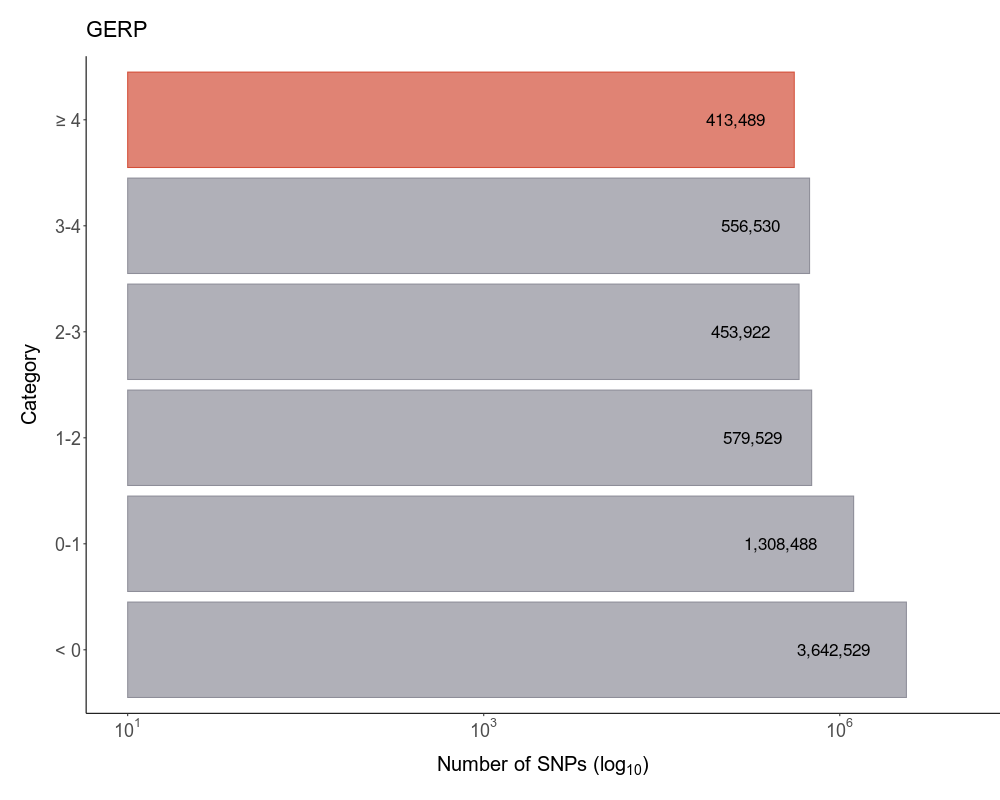
\includegraphics[keepaspectratio]{qmd/../plots/main/fig_2a.png}}

}

\caption{Total load results}

\end{figure}%

\begin{Shaded}
\begin{Highlighting}[]
\FunctionTok{library}\NormalTok{(readxl); }\FunctionTok{library}\NormalTok{(dplyr); }\FunctionTok{library}\NormalTok{(kableExtra)}
\NormalTok{totals }\OtherTok{\textless{}{-}} \FunctionTok{read.csv}\NormalTok{(}\StringTok{"../output/models/intervals/total\_gerp45\_high.csv"}\NormalTok{)}
\NormalTok{totals }\SpecialCharTok{\%\textgreater{}\%} \FunctionTok{kbl}\NormalTok{() }
\end{Highlighting}
\end{Shaded}

\begin{tabular}[t]{l|r|r|l|r|r|r|r|r|l}
\hline
parameter & outer\_width & inner\_width & point\_est & ll & l & m & h & hh & model\\
\hline
b\_scaletotal\_load & 0.95 & 0.8 & median & -0.27 & -0.25 & -0.21 & -0.17 & -0.14 & GERP\\
\hline
b\_scaletotal\_load & 0.95 & 0.8 & median & -0.18 & -0.16 & -0.11 & -0.06 & -0.04 & SnpEff\\
\hline
\end{tabular}

We also find significant effects of both hom and het GERP and SnpEff
load:

\begin{figure}[H]

{\centering \pandocbounded{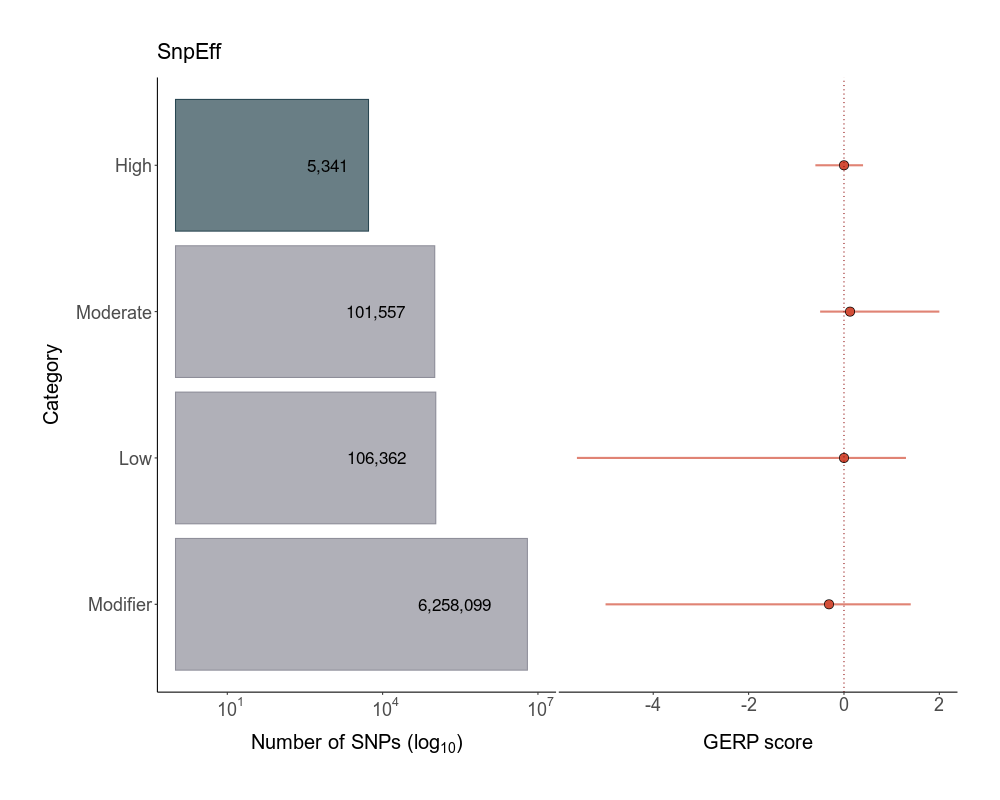
\includegraphics[keepaspectratio]{qmd/../plots/main/fig_2b.png}}

}

\caption{Hom het load results}

\end{figure}%

\begin{Shaded}
\begin{Highlighting}[]
\NormalTok{homhet }\OtherTok{\textless{}{-}} \FunctionTok{read.csv}\NormalTok{(}\StringTok{"../output/models/intervals/hom\_het\_gerp45\_high.csv"}\NormalTok{)}
\NormalTok{homhet }\SpecialCharTok{\%\textgreater{}\%} \FunctionTok{kbl}\NormalTok{() }
\end{Highlighting}
\end{Shaded}

\begin{tabular}[t]{l|r|r|l|r|r|r|r|r|l|l}
\hline
parameter & outer\_width & inner\_width & point\_est & ll & l & m & h & hh & model & loadtype\\
\hline
b\_scalehom\_load & 0.95 & 0.8 & median & -0.76 & -0.70 & -0.57 & -0.45 & -0.39 & Hom & GERP\\
\hline
b\_scalehet\_load & 0.95 & 0.8 & median & -0.78 & -0.72 & -0.60 & -0.48 & -0.41 & Het & GERP\\
\hline
b\_scalehom\_load & 0.95 & 0.8 & median & -0.17 & -0.15 & -0.09 & -0.04 & -0.01 & Hom & SnpEff\\
\hline
b\_scalehet\_load & 0.95 & 0.8 & median & -0.24 & -0.21 & -0.15 & -0.09 & -0.06 & Het & SnpEff\\
\hline
\end{tabular}

Here you can find the posterior distributions of model set 1 (load on
traits) for GERP :
\pandocbounded{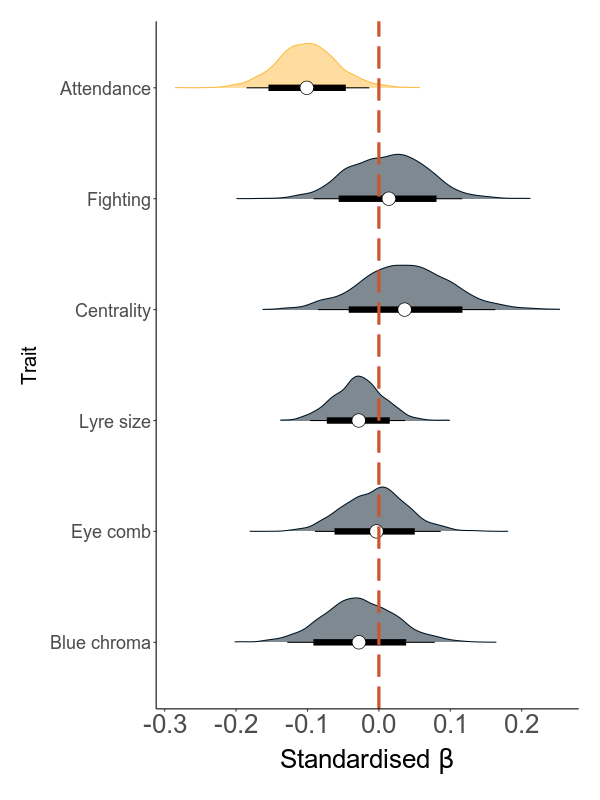
\includegraphics[keepaspectratio]{qmd/../plots/main/fig_4_left_load_traits.png}}

\begin{figure}[H]

{\centering \pandocbounded{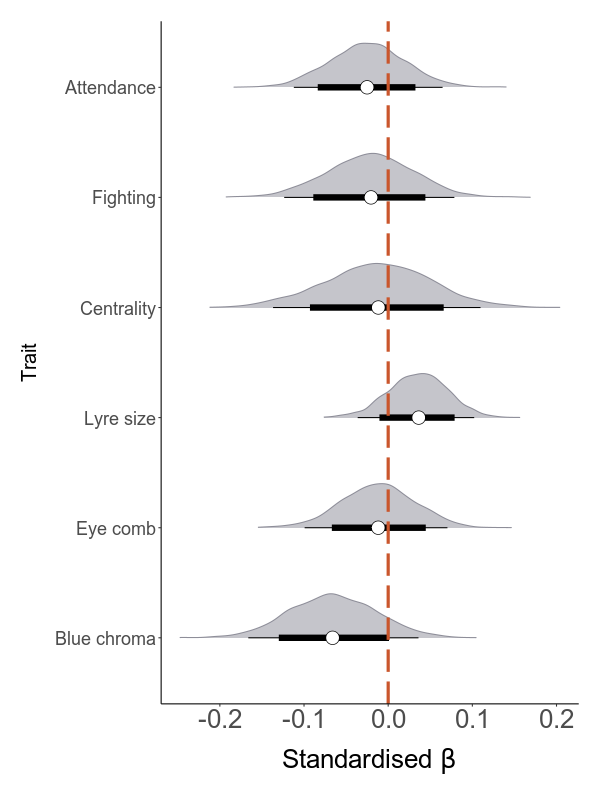
\includegraphics[keepaspectratio]{qmd/../plots/extended/extended_7_high_left_load_traits.png}}

}

\caption{MS set 1 results SnpEff}

\end{figure}%

And for model set 2 (traits on MS) for GERP and SnpEff:
\pandocbounded{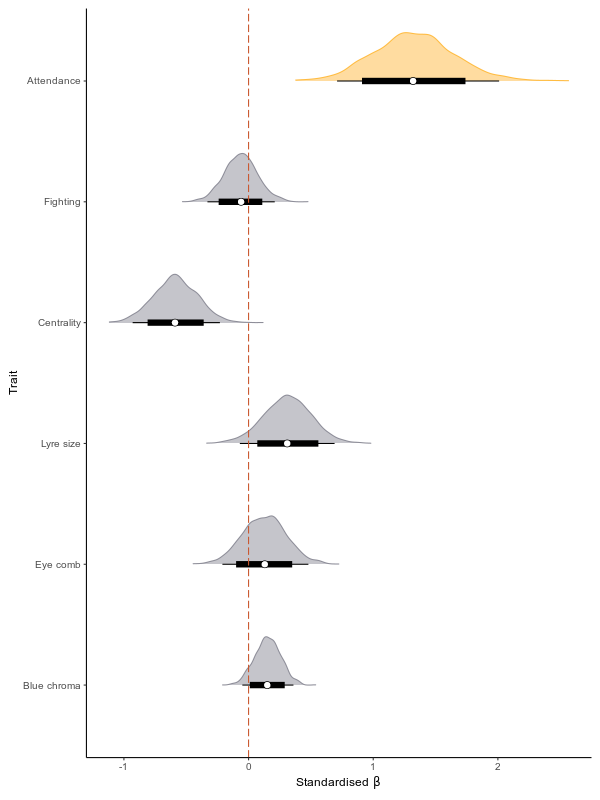
\includegraphics[keepaspectratio]{qmd/../plots/main/fig_4_right_traits_ams.png}}
\pandocbounded{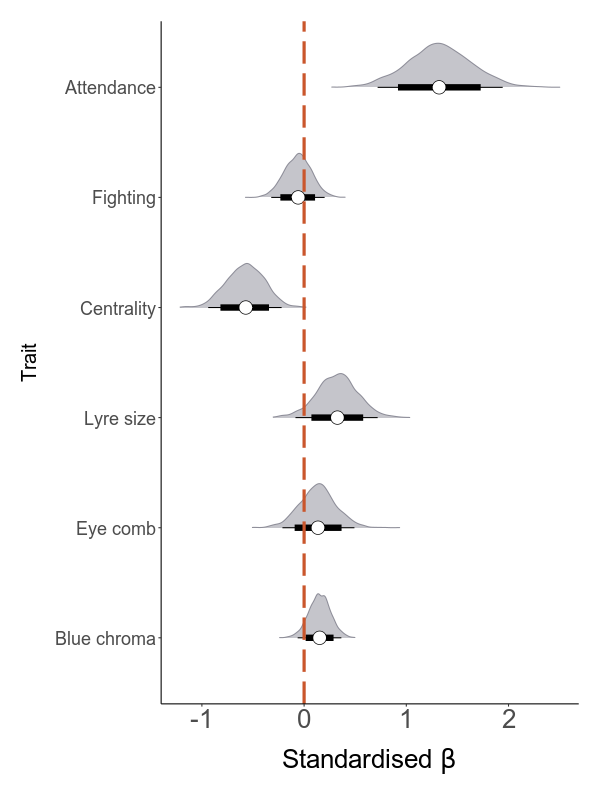
\includegraphics[keepaspectratio]{qmd/../plots/extended/extended_7_high_right_traits_ams.png}}

We can check out the result of the direct and indirect effects as
follows:

\begin{Shaded}
\begin{Highlighting}[]
\NormalTok{effects }\OtherTok{\textless{}{-}} \FunctionTok{read.csv}\NormalTok{(}\StringTok{"../output/models/annual/direct\_indirect\_summary.csv"}\NormalTok{)}
\NormalTok{effects }\SpecialCharTok{\%\textgreater{}\%} \FunctionTok{kbl}\NormalTok{() }\SpecialCharTok{\%\textgreater{}\%}  \FunctionTok{kable\_classic\_2}\NormalTok{() }\SpecialCharTok{\%\textgreater{}\%} \FunctionTok{scroll\_box}\NormalTok{(}\AttributeTok{width =} \StringTok{"99\%"}\NormalTok{, }\AttributeTok{height =} \StringTok{"200px"}\NormalTok{)}
\end{Highlighting}
\end{Shaded}

\begin{table}
\centering
\begin{tabular}[t]{l|l|l|r|r|r|r|r|r|r|r|r|r|r|r|r|r|r|r|r|r|r}
\hline
treatment & mediator & method & indirect\_median & indirect\_lower & indirect\_upper & direct\_median & direct\_lower & direct\_upper & total\_median & total\_lower & total\_upper & path1\_median & path1\_lower & path1\_upper & path2\_median & path2\_lower & path2\_upper & indirect\_lower\_80 & indirect\_upper\_80 & direct\_lower\_80 & direct\_upper\_80\\
\hline
b\_scaletotal\_load & b\_scalelyre & gerp45 & -0.01 & -0.04 & 0.01 & -0.13 & -0.36 & 0.11 & -0.14 & -0.38 & 0.10 & -0.03 & -0.10 & 0.04 & 0.31 & -0.07 & 0.69 & -0.03 & 0.01 & -0.29 & 0.03\\
\hline
b\_scaletotal\_load & b\_scaleeyec & gerp45 & 0.00 & -0.02 & 0.02 & -0.13 & -0.36 & 0.11 & -0.13 & -0.36 & 0.11 & 0.00 & -0.09 & 0.09 & 0.13 & -0.21 & 0.48 & -0.01 & 0.01 & -0.29 & 0.03\\
\hline
b\_scaletotal\_load & b\_scaleblue & gerp45 & 0.00 & -0.03 & 0.01 & -0.13 & -0.36 & 0.11 & -0.14 & -0.38 & 0.10 & -0.03 & -0.13 & 0.08 & 0.15 & -0.05 & 0.36 & -0.02 & 0.01 & -0.29 & 0.03\\
\hline
b\_scaletotal\_load & b\_scaleattend & gerp45 & -0.13 & -0.28 & -0.01 & -0.13 & -0.36 & 0.11 & -0.26 & -0.54 & 0.01 & -0.10 & -0.19 & -0.01 & 1.32 & 0.71 & 2.01 & -0.22 & -0.05 & -0.29 & 0.03\\
\hline
b\_scaletotal\_load & b\_scalefight & gerp45 & 0.00 & -0.02 & 0.02 & -0.13 & -0.36 & 0.11 & -0.13 & -0.36 & 0.11 & 0.01 & -0.09 & 0.12 & -0.06 & -0.33 & 0.21 & -0.01 & 0.01 & -0.29 & 0.03\\
\hline
b\_scaletotal\_load & b\_scaledist & gerp45 & -0.02 & -0.11 & 0.05 & -0.13 & -0.36 & 0.11 & -0.15 & -0.41 & 0.11 & 0.04 & -0.09 & 0.16 & -0.59 & -0.93 & -0.23 & -0.07 & 0.02 & -0.29 & 0.03\\
\hline
b\_scaletotal\_load & b\_scalelyre & high & 0.01 & -0.01 & 0.05 & -0.11 & -0.38 & 0.16 & -0.09 & -0.37 & 0.18 & 0.04 & -0.04 & 0.10 & 0.33 & -0.08 & 0.72 & 0.00 & 0.03 & -0.27 & 0.06\\
\hline
b\_scaletotal\_load & b\_scaleeyec & high & 0.00 & -0.03 & 0.02 & -0.11 & -0.38 & 0.16 & -0.11 & -0.38 & 0.16 & -0.01 & -0.10 & 0.07 & 0.14 & -0.21 & 0.49 & -0.01 & 0.01 & -0.27 & 0.06\\
\hline
b\_scaletotal\_load & b\_scaleblue & high & -0.01 & -0.04 & 0.01 & -0.11 & -0.38 & 0.16 & -0.12 & -0.39 & 0.15 & -0.07 & -0.17 & 0.04 & 0.15 & -0.06 & 0.36 & -0.03 & 0.00 & -0.27 & 0.06\\
\hline
b\_scaletotal\_load & b\_scaleattend & high & -0.03 & -0.16 & 0.09 & -0.11 & -0.38 & 0.16 & -0.14 & -0.44 & 0.15 & -0.03 & -0.11 & 0.06 & 1.32 & 0.72 & 1.94 & -0.11 & 0.04 & -0.27 & 0.06\\
\hline
b\_scaletotal\_load & b\_scalefight & high & 0.00 & -0.01 & 0.02 & -0.11 & -0.38 & 0.16 & -0.10 & -0.38 & 0.17 & -0.02 & -0.12 & 0.08 & -0.06 & -0.32 & 0.20 & -0.01 & 0.01 & -0.27 & 0.06\\
\hline
b\_scaletotal\_load & b\_scaledist & high & 0.01 & -0.06 & 0.09 & -0.11 & -0.38 & 0.16 & -0.10 & -0.39 & 0.17 & -0.01 & -0.14 & 0.11 & -0.57 & -0.94 & -0.22 & -0.04 & 0.06 & -0.27 & 0.06\\
\hline
\end{tabular}
\end{table}

\bookmarksetup{startatroot}

\chapter{Load per genomic region}\label{load-per-genomic-region}

\section{Introduction}\label{introduction-5}

Both functional noncoding and protein-coding regions can be under
selective constraint. However, the former include various regulatory
elements such as promoters, enhancers and silencers, which play
different roles in gene regulation and might therefore be expected to
experience different strengths of purifying selection. To investigate
whether the fitness effects of deleterious mutations vary by genomic
region, we classified each deleterious mutation according to whether it
was located within a promoter, transcription start site, intron or exon.
Then, we calculate total load based on these subsets and model their
effects on LMS.

\subsection{Genomic regions}\label{genomic-regions}

We use a combination of GenomicRanges and rtracklayer and other packages
to divide up the genome annotation file into the four genomic regions.

\subsubsection{Subset reference genome}\label{subset-reference-genome}

\begin{Shaded}
\begin{Highlighting}[]
\DocumentationTok{\#\#\#\# Packages \#\#\#\#\#}
\NormalTok{pacman}\SpecialCharTok{::}\FunctionTok{p\_load}\NormalTok{(BiocManager, rtracklayer, GenomicFeatures, BiocGenerics, data.table, dplyr, genomation, GenomicRanges, tibble)}

\DocumentationTok{\#\#\#\# Genome data \#\#\#\#}
\CommentTok{\# first change scaffold names}
\NormalTok{gff\_raw }\OtherTok{\textless{}{-}} \FunctionTok{fread}\NormalTok{(}\StringTok{"data/genomic/annotation/PO2979\_Lyrurus\_tetrix\_black\_grouse.annotation.gff"}\NormalTok{) }
\NormalTok{gff\_raw}\SpecialCharTok{$}\NormalTok{V1 }\OtherTok{\textless{}{-}} \FunctionTok{gsub}\NormalTok{(}\StringTok{";"}\NormalTok{, }\StringTok{"\_\_"}\NormalTok{, gff\_raw}\SpecialCharTok{$}\NormalTok{V1)}
\NormalTok{gff\_raw}\SpecialCharTok{$}\NormalTok{V1 }\OtherTok{\textless{}{-}} \FunctionTok{gsub}\NormalTok{(}\StringTok{"="}\NormalTok{, }\StringTok{"\_"}\NormalTok{, gff\_raw}\SpecialCharTok{$}\NormalTok{V1)}
\FunctionTok{write.table}\NormalTok{(gff\_raw, }\AttributeTok{file =} \StringTok{"data/genomic/PO2979\_Lyrurus\_tetrix\_black\_grouse.annotation\_editedscafnames.gff"}\NormalTok{, }\AttributeTok{sep =} \StringTok{"}\SpecialCharTok{\textbackslash{}t}\StringTok{"}\NormalTok{, }\AttributeTok{col.names =} \ConstantTok{FALSE}\NormalTok{, }\AttributeTok{quote=}\NormalTok{F, }\AttributeTok{row.names =} \ConstantTok{FALSE}\NormalTok{)}

\CommentTok{\#read in new file}
\NormalTok{gff }\OtherTok{\textless{}{-}} \FunctionTok{makeTxDbFromGFF}\NormalTok{(}\StringTok{"data/genomic/PO2979\_Lyrurus\_tetrix\_black\_grouse.annotation\_editedscafnames.gff"}\NormalTok{, }\AttributeTok{format=}\StringTok{"gff3"}\NormalTok{, }\AttributeTok{organism=}\StringTok{"Lyrurus tetrix"}\NormalTok{) }

\DocumentationTok{\#\# divide up between the 4 regions }\AlertTok{\#\#\#}

\NormalTok{promoters }\OtherTok{\textless{}{-}} \FunctionTok{promoters}\NormalTok{(gff, }\AttributeTok{upstream=}\DecValTok{2000}\NormalTok{, }\AttributeTok{downstream=}\DecValTok{200}\NormalTok{, }\AttributeTok{columns=}\FunctionTok{c}\NormalTok{(}\StringTok{"tx\_name"}\NormalTok{, }\StringTok{"gene\_id"}\NormalTok{)) }\CommentTok{\# From NIOO}
\NormalTok{TSS }\OtherTok{\textless{}{-}} \FunctionTok{promoters}\NormalTok{(gff, }\AttributeTok{upstream=}\DecValTok{300}\NormalTok{, }\AttributeTok{downstream=}\DecValTok{50}\NormalTok{, }\AttributeTok{columns=}\FunctionTok{c}\NormalTok{(}\StringTok{"tx\_name"}\NormalTok{, }\StringTok{"gene\_id"}\NormalTok{)) }\CommentTok{\# TSS as in Laine et al., 2016. Nature Communications}
\NormalTok{exons\_gene }\OtherTok{\textless{}{-}} \FunctionTok{unlist}\NormalTok{(}\FunctionTok{exonsBy}\NormalTok{(gff, }\StringTok{"gene"}\NormalTok{)) }\CommentTok{\# group exons by genes}
\NormalTok{introns }\OtherTok{\textless{}{-}} \FunctionTok{unlist}\NormalTok{(}\FunctionTok{intronsByTranscript}\NormalTok{(gff, }\AttributeTok{use.names=}\ConstantTok{TRUE}\NormalTok{))}

\DocumentationTok{\#\#\# write out files}
\FunctionTok{export}\NormalTok{(promoters, }\StringTok{"data/genomic/annotation/promoters.gff3"}\NormalTok{)}
\FunctionTok{export}\NormalTok{(TSS, }\StringTok{"data/genomic/annotation/TSS.gff3"}\NormalTok{)}
\NormalTok{introns}\SpecialCharTok{@}\NormalTok{ranges}\SpecialCharTok{@}\NormalTok{NAMES[}\FunctionTok{is.na}\NormalTok{(introns}\SpecialCharTok{@}\NormalTok{ranges}\SpecialCharTok{@}\NormalTok{NAMES)]}\OtherTok{\textless{}{-}}\StringTok{"Unknown"}
\FunctionTok{export}\NormalTok{(introns, }\StringTok{"data/genomic/annotation/introns\_transcripts.gff3"}\NormalTok{)}
\FunctionTok{export}\NormalTok{(exons\_gene, }\StringTok{"data/genomic/annotation/exons\_gene.gff3"}\NormalTok{)}
\end{Highlighting}
\end{Shaded}

\subsubsection{Annotate deleterious
mutations}\label{annotate-deleterious-mutations}

Then, we load in all deleterious mutations for GERP and SnpEff
separately and annotate the mutations according to the four regions.

\begin{Shaded}
\begin{Highlighting}[]
\DocumentationTok{\#\#\#\#\#\# Annotate high impact and GERP mutations \#\#\#\#\#}
\DocumentationTok{\#\#\# annotate gene regions per SNP for high impact and gerp mutations }\AlertTok{\#\#\#}

\DocumentationTok{\#\#\# load data }\AlertTok{\#\#\#}

\FunctionTok{load}\NormalTok{(}\AttributeTok{file =} \StringTok{"output/load/snpeff/snpeff\_high.RData"}\NormalTok{)}
\FunctionTok{load}\NormalTok{(}\AttributeTok{file =} \StringTok{"output/load/gerp/gerp\_over4.RData"}\NormalTok{)}

\DocumentationTok{\#\#\# change scaf names}
\NormalTok{snpeff}\SpecialCharTok{$}\NormalTok{CHROM }\OtherTok{\textless{}{-}} \FunctionTok{gsub}\NormalTok{(}\StringTok{";"}\NormalTok{, }\StringTok{"\_\_"}\NormalTok{, snpeff}\SpecialCharTok{$}\NormalTok{CHROM)}
\NormalTok{snpeff}\SpecialCharTok{$}\NormalTok{CHROM }\OtherTok{\textless{}{-}} \FunctionTok{gsub}\NormalTok{(}\StringTok{"="}\NormalTok{, }\StringTok{"\_"}\NormalTok{, snpeff}\SpecialCharTok{$}\NormalTok{CHROM)}

\NormalTok{gerp}\SpecialCharTok{$}\NormalTok{chr }\OtherTok{\textless{}{-}} \FunctionTok{gsub}\NormalTok{(}\StringTok{";"}\NormalTok{, }\StringTok{"\_\_"}\NormalTok{, gerp}\SpecialCharTok{$}\NormalTok{chr)}
\NormalTok{gerp}\SpecialCharTok{$}\NormalTok{chr }\OtherTok{\textless{}{-}} \FunctionTok{gsub}\NormalTok{(}\StringTok{"="}\NormalTok{, }\StringTok{"\_"}\NormalTok{, gerp}\SpecialCharTok{$}\NormalTok{chr)}

\DocumentationTok{\#\#\# remove genotypes: not necessary here}
\NormalTok{snpeff }\OtherTok{\textless{}{-}}\NormalTok{ snpeff[,}\FunctionTok{c}\NormalTok{(}\DecValTok{1}\SpecialCharTok{:}\DecValTok{9}\NormalTok{)]}
\NormalTok{gerp }\OtherTok{\textless{}{-}}\NormalTok{ gerp[,}\FunctionTok{c}\NormalTok{(}\DecValTok{1}\SpecialCharTok{:}\DecValTok{9}\NormalTok{)]}

\DocumentationTok{\#\#\#\#\#\#\# Gene regions \#\#\#\#\#\#\#\#\#\#\#}

\DocumentationTok{\#\#\# load annotation data}
\NormalTok{annotation\_dir }\OtherTok{\textless{}{-}} \StringTok{"data/genomic/annotation"}

\NormalTok{promoter}\OtherTok{=}\FunctionTok{unique}\NormalTok{(}\FunctionTok{gffToGRanges}\NormalTok{(}\FunctionTok{paste0}\NormalTok{(annotation\_dir, }\StringTok{"/promoters.gff3"}\NormalTok{)))}
\NormalTok{TSS}\OtherTok{=}\FunctionTok{unique}\NormalTok{(}\FunctionTok{gffToGRanges}\NormalTok{(}\FunctionTok{paste0}\NormalTok{(annotation\_dir, }\StringTok{"/TSS.gff3"}\NormalTok{)))}
\NormalTok{introns}\OtherTok{=}\FunctionTok{unique}\NormalTok{(}\FunctionTok{gffToGRanges}\NormalTok{(}\FunctionTok{paste0}\NormalTok{(annotation\_dir, }\StringTok{"/introns\_transcripts.gff3"}\NormalTok{)))}
\NormalTok{exons\_gene}\OtherTok{=}\FunctionTok{unique}\NormalTok{(}\FunctionTok{gffToGRanges}\NormalTok{(}\FunctionTok{paste0}\NormalTok{(annotation\_dir, }\StringTok{"/exons\_gene.gff3"}\NormalTok{)))}

\DocumentationTok{\#\#\#\# Annotate SNPeff regions \#\#\#\#}
\NormalTok{snpeff}\SpecialCharTok{$}\NormalTok{end }\OtherTok{\textless{}{-}}\NormalTok{ snpeff}\SpecialCharTok{$}\NormalTok{POS}
\NormalTok{snpeff}\SpecialCharTok{$}\NormalTok{start }\OtherTok{\textless{}{-}}\NormalTok{ snpeff}\SpecialCharTok{$}\NormalTok{POS}
\NormalTok{snpef\_gr }\OtherTok{\textless{}{-}} \FunctionTok{as}\NormalTok{(snpeff, }\StringTok{"GRanges"}\NormalTok{)}

\NormalTok{snpef\_promoter }\OtherTok{\textless{}{-}} \FunctionTok{as.data.frame}\NormalTok{(}\FunctionTok{subsetByOverlaps}\NormalTok{(snpef\_gr, promoter)) }\SpecialCharTok{\%\textgreater{}\%}
  \FunctionTok{add\_column}\NormalTok{(}\StringTok{"region\_promoter"} \OtherTok{=} \DecValTok{1}\NormalTok{) }\SpecialCharTok{\%\textgreater{}\%}\NormalTok{ dplyr}\SpecialCharTok{::}\FunctionTok{rename}\NormalTok{(}\AttributeTok{chr =}\NormalTok{ seqnames)}\SpecialCharTok{\%\textgreater{}\%} \FunctionTok{unique}\NormalTok{()}

\NormalTok{snpef\_TSS }\OtherTok{\textless{}{-}} \FunctionTok{as.data.frame}\NormalTok{(}\FunctionTok{subsetByOverlaps}\NormalTok{(snpef\_gr, TSS))}\SpecialCharTok{\%\textgreater{}\%}
  \FunctionTok{add\_column}\NormalTok{(}\StringTok{"region\_tss"} \OtherTok{=} \DecValTok{1}\NormalTok{) }\SpecialCharTok{\%\textgreater{}\%}\NormalTok{ dplyr}\SpecialCharTok{::}\FunctionTok{rename}\NormalTok{(}\AttributeTok{chr =}\NormalTok{ seqnames)}\SpecialCharTok{\%\textgreater{}\%} \FunctionTok{unique}\NormalTok{()}

\NormalTok{snpef\_exons }\OtherTok{\textless{}{-}} \FunctionTok{as.data.frame}\NormalTok{(}\FunctionTok{subsetByOverlaps}\NormalTok{(snpef\_gr, exons\_gene))}\SpecialCharTok{\%\textgreater{}\%}
  \FunctionTok{add\_column}\NormalTok{(}\StringTok{"region\_exon"} \OtherTok{=} \DecValTok{1}\NormalTok{) }\SpecialCharTok{\%\textgreater{}\%}\NormalTok{ dplyr}\SpecialCharTok{::}\FunctionTok{rename}\NormalTok{(}\AttributeTok{chr =}\NormalTok{ seqnames)}\SpecialCharTok{\%\textgreater{}\%} \FunctionTok{unique}\NormalTok{()}

\NormalTok{snpef\_introns }\OtherTok{\textless{}{-}} \FunctionTok{as.data.frame}\NormalTok{(}\FunctionTok{subsetByOverlaps}\NormalTok{(snpef\_gr, introns))}\SpecialCharTok{\%\textgreater{}\%}
  \FunctionTok{add\_column}\NormalTok{(}\StringTok{"region\_intron"} \OtherTok{=} \DecValTok{1}\NormalTok{) }\SpecialCharTok{\%\textgreater{}\%}\NormalTok{ dplyr}\SpecialCharTok{::}\FunctionTok{rename}\NormalTok{(}\AttributeTok{chr =}\NormalTok{ seqnames)}\SpecialCharTok{\%\textgreater{}\%} \FunctionTok{unique}\NormalTok{()}

\NormalTok{snpef\_all }\OtherTok{\textless{}{-}} \FunctionTok{left\_join}\NormalTok{(snpeff, snpef\_promoter[,}\FunctionTok{c}\NormalTok{(}\StringTok{"chr"}\NormalTok{, }\StringTok{"start"}\NormalTok{, }\StringTok{"region\_promoter"}\NormalTok{)], }\AttributeTok{by =} \FunctionTok{c}\NormalTok{(}\StringTok{"CHROM"} \OtherTok{=} \StringTok{"chr"}\NormalTok{, }\StringTok{"start"}\NormalTok{))}\SpecialCharTok{\%\textgreater{}\%}
  \FunctionTok{left\_join}\NormalTok{(snpef\_TSS[,}\FunctionTok{c}\NormalTok{(}\StringTok{"chr"}\NormalTok{, }\StringTok{"start"}\NormalTok{, }\StringTok{"region\_tss"}\NormalTok{)], }\AttributeTok{by =} \FunctionTok{c}\NormalTok{(}\StringTok{"CHROM"} \OtherTok{=} \StringTok{"chr"}\NormalTok{, }\StringTok{"start"}\NormalTok{))}\SpecialCharTok{\%\textgreater{}\%}
  \FunctionTok{left\_join}\NormalTok{(snpef\_exons[,}\FunctionTok{c}\NormalTok{(}\StringTok{"chr"}\NormalTok{, }\StringTok{"start"}\NormalTok{, }\StringTok{"region\_exon"}\NormalTok{)], }\AttributeTok{by =} \FunctionTok{c}\NormalTok{(}\StringTok{"CHROM"} \OtherTok{=} \StringTok{"chr"}\NormalTok{, }\StringTok{"start"}\NormalTok{))}\SpecialCharTok{\%\textgreater{}\%}
  \FunctionTok{left\_join}\NormalTok{(snpef\_introns[,}\FunctionTok{c}\NormalTok{(}\StringTok{"chr"}\NormalTok{, }\StringTok{"start"}\NormalTok{, }\StringTok{"region\_intron"}\NormalTok{)], }\AttributeTok{by =} \FunctionTok{c}\NormalTok{(}\StringTok{"CHROM"} \OtherTok{=} \StringTok{"chr"}\NormalTok{, }\StringTok{"start"}\NormalTok{))}

\CommentTok{\# correct promoters}
\NormalTok{snpef\_all }\OtherTok{\textless{}{-}}\NormalTok{ snpef\_all }\SpecialCharTok{\%\textgreater{}\%} \FunctionTok{mutate}\NormalTok{(}\AttributeTok{region\_promoter =} \FunctionTok{case\_when}\NormalTok{(}
\NormalTok{  region\_tss }\SpecialCharTok{==} \DecValTok{1} \SpecialCharTok{\&}\NormalTok{ region\_promoter }\SpecialCharTok{==} \DecValTok{1} \SpecialCharTok{\textasciitilde{}} \ConstantTok{NA}\NormalTok{,}
  \FunctionTok{is.na}\NormalTok{(region\_tss) }\SpecialCharTok{\&}\NormalTok{ region\_promoter }\SpecialCharTok{==} \DecValTok{1} \SpecialCharTok{\textasciitilde{}} \DecValTok{1}
\NormalTok{))}

\FunctionTok{save}\NormalTok{(snpef\_all, }\AttributeTok{file =} \StringTok{"output/load/snpeff/snpeff\_high\_annotated\_region.RData"}\NormalTok{)}

\DocumentationTok{\#\#\#\# Annotate gerp regions \#\#\#\#}
\NormalTok{gerp}\SpecialCharTok{$}\NormalTok{end }\OtherTok{\textless{}{-}}\NormalTok{ gerp}\SpecialCharTok{$}\NormalTok{pos}
\NormalTok{gerp}\SpecialCharTok{$}\NormalTok{start }\OtherTok{\textless{}{-}}\NormalTok{ gerp}\SpecialCharTok{$}\NormalTok{pos}
\NormalTok{gerp\_gr }\OtherTok{\textless{}{-}} \FunctionTok{as}\NormalTok{(gerp, }\StringTok{"GRanges"}\NormalTok{)}

\NormalTok{gerp\_promoter }\OtherTok{\textless{}{-}} \FunctionTok{as.data.frame}\NormalTok{(}\FunctionTok{subsetByOverlaps}\NormalTok{(gerp\_gr, promoter)) }\SpecialCharTok{\%\textgreater{}\%}
  \FunctionTok{add\_column}\NormalTok{(}\StringTok{"region\_promoter"} \OtherTok{=} \DecValTok{1}\NormalTok{) }\SpecialCharTok{\%\textgreater{}\%}\NormalTok{ dplyr}\SpecialCharTok{::}\FunctionTok{rename}\NormalTok{(}\AttributeTok{chr =}\NormalTok{ seqnames)}\SpecialCharTok{\%\textgreater{}\%} \FunctionTok{unique}\NormalTok{()}

\NormalTok{gerp\_TSS }\OtherTok{\textless{}{-}} \FunctionTok{as.data.frame}\NormalTok{(}\FunctionTok{subsetByOverlaps}\NormalTok{(gerp\_gr, TSS))}\SpecialCharTok{\%\textgreater{}\%}
  \FunctionTok{add\_column}\NormalTok{(}\StringTok{"region\_tss"} \OtherTok{=} \DecValTok{1}\NormalTok{) }\SpecialCharTok{\%\textgreater{}\%}\NormalTok{ dplyr}\SpecialCharTok{::}\FunctionTok{rename}\NormalTok{(}\AttributeTok{chr =}\NormalTok{ seqnames)}\SpecialCharTok{\%\textgreater{}\%} \FunctionTok{unique}\NormalTok{()}

\NormalTok{gerp\_exons }\OtherTok{\textless{}{-}} \FunctionTok{as.data.frame}\NormalTok{(}\FunctionTok{subsetByOverlaps}\NormalTok{(gerp\_gr, exons\_gene))}\SpecialCharTok{\%\textgreater{}\%}
  \FunctionTok{add\_column}\NormalTok{(}\StringTok{"region\_exon"} \OtherTok{=} \DecValTok{1}\NormalTok{) }\SpecialCharTok{\%\textgreater{}\%}\NormalTok{ dplyr}\SpecialCharTok{::}\FunctionTok{rename}\NormalTok{(}\AttributeTok{chr =}\NormalTok{ seqnames)}\SpecialCharTok{\%\textgreater{}\%} \FunctionTok{unique}\NormalTok{()}

\NormalTok{gerp\_introns }\OtherTok{\textless{}{-}} \FunctionTok{as.data.frame}\NormalTok{(}\FunctionTok{subsetByOverlaps}\NormalTok{(gerp\_gr, introns))}\SpecialCharTok{\%\textgreater{}\%}
  \FunctionTok{add\_column}\NormalTok{(}\StringTok{"region\_intron"} \OtherTok{=} \DecValTok{1}\NormalTok{) }\SpecialCharTok{\%\textgreater{}\%}\NormalTok{ dplyr}\SpecialCharTok{::}\FunctionTok{rename}\NormalTok{(}\AttributeTok{chr =}\NormalTok{ seqnames)}\SpecialCharTok{\%\textgreater{}\%} \FunctionTok{unique}\NormalTok{()}

\NormalTok{gerp\_all }\OtherTok{\textless{}{-}} \FunctionTok{left\_join}\NormalTok{(gerp, gerp\_promoter[,}\FunctionTok{c}\NormalTok{(}\StringTok{"chr"}\NormalTok{, }\StringTok{"start"}\NormalTok{, }\StringTok{"region\_promoter"}\NormalTok{)], }\AttributeTok{by =} \FunctionTok{c}\NormalTok{(}\StringTok{"chr"} \OtherTok{=} \StringTok{"chr"}\NormalTok{, }\StringTok{"start"}\NormalTok{))}\SpecialCharTok{\%\textgreater{}\%}
   \FunctionTok{left\_join}\NormalTok{(gerp\_TSS[,}\FunctionTok{c}\NormalTok{(}\StringTok{"chr"}\NormalTok{, }\StringTok{"start"}\NormalTok{, }\StringTok{"region\_tss"}\NormalTok{)], }\AttributeTok{by =} \FunctionTok{c}\NormalTok{(}\StringTok{"chr"} \OtherTok{=} \StringTok{"chr"}\NormalTok{, }\StringTok{"start"}\NormalTok{))}\SpecialCharTok{\%\textgreater{}\%}
  \FunctionTok{left\_join}\NormalTok{(gerp\_exons[,}\FunctionTok{c}\NormalTok{(}\StringTok{"chr"}\NormalTok{, }\StringTok{"start"}\NormalTok{, }\StringTok{"region\_exon"}\NormalTok{)], }\AttributeTok{by =} \FunctionTok{c}\NormalTok{(}\StringTok{"chr"} \OtherTok{=} \StringTok{"chr"}\NormalTok{, }\StringTok{"start"}\NormalTok{))}\SpecialCharTok{\%\textgreater{}\%}
  \FunctionTok{left\_join}\NormalTok{(gerp\_introns[,}\FunctionTok{c}\NormalTok{(}\StringTok{"chr"}\NormalTok{, }\StringTok{"start"}\NormalTok{, }\StringTok{"region\_intron"}\NormalTok{)], }\AttributeTok{by =} \FunctionTok{c}\NormalTok{(}\StringTok{"chr"} \OtherTok{=} \StringTok{"chr"}\NormalTok{, }\StringTok{"start"}\NormalTok{))}
 
\CommentTok{\# correct promoters}
\NormalTok{gerp\_all }\OtherTok{\textless{}{-}}\NormalTok{ gerp\_all }\SpecialCharTok{\%\textgreater{}\%} \FunctionTok{mutate}\NormalTok{(}\AttributeTok{region\_promoter =} \FunctionTok{case\_when}\NormalTok{(}
\NormalTok{  region\_tss }\SpecialCharTok{==} \DecValTok{1} \SpecialCharTok{\&}\NormalTok{ region\_promoter }\SpecialCharTok{==} \DecValTok{1} \SpecialCharTok{\textasciitilde{}} \ConstantTok{NA}\NormalTok{,}
  \FunctionTok{is.na}\NormalTok{(region\_tss) }\SpecialCharTok{\&}\NormalTok{ region\_promoter }\SpecialCharTok{==} \DecValTok{1} \SpecialCharTok{\textasciitilde{}} \DecValTok{1}
\NormalTok{))}

\FunctionTok{save}\NormalTok{(gerp\_all, }\AttributeTok{file =} \StringTok{"output/load/gerp/gerp\_annotated\_region.RData"}\NormalTok{)}
\end{Highlighting}
\end{Shaded}

\subsubsection{Calculate mutation load}\label{calculate-mutation-load}

These two files (gerp\_all and snpeff\_all) contain the SNP locations
and additional binary columns whether the mutations was located in one
of the 4 regions. We can use this file together with the files
containing the genotypes to calculate mutation load based on the subsets
of mutations only.

\begin{Shaded}
\begin{Highlighting}[]
\DocumentationTok{\#\#\#\# Calculate load per region \#\#\#\#\#}

\CommentTok{\# load annotated gerp data}
\FunctionTok{load}\NormalTok{(}\AttributeTok{file =} \StringTok{"output/load/gerp/gerp\_annotated\_region.RData"}\NormalTok{)}
\NormalTok{gerp\_all}\SpecialCharTok{$}\NormalTok{chr }\OtherTok{\textless{}{-}} \FunctionTok{gsub}\NormalTok{(}\StringTok{"\_\_"}\NormalTok{, }\StringTok{";"}\NormalTok{, gerp\_all}\SpecialCharTok{$}\NormalTok{chr)}
\NormalTok{gerp\_all}\SpecialCharTok{$}\NormalTok{chr }\OtherTok{\textless{}{-}} \FunctionTok{gsub}\NormalTok{(}\StringTok{"HRSCAF\_"}\NormalTok{, }\StringTok{"HRSCAF="}\NormalTok{, gerp\_all}\SpecialCharTok{$}\NormalTok{chr)}

\CommentTok{\# load annotation}
\FunctionTok{load}\NormalTok{(}\AttributeTok{file =} \StringTok{"output/load/snpeff/snpeff\_high\_annotated\_region.RData"}\NormalTok{)}
\NormalTok{snpef\_all}\SpecialCharTok{$}\NormalTok{CHROM }\OtherTok{\textless{}{-}} \FunctionTok{gsub}\NormalTok{(}\StringTok{"\_\_"}\NormalTok{, }\StringTok{";"}\NormalTok{, snpef\_all}\SpecialCharTok{$}\NormalTok{CHROM)}
\NormalTok{snpef\_all}\SpecialCharTok{$}\NormalTok{CHROM }\OtherTok{\textless{}{-}} \FunctionTok{gsub}\NormalTok{(}\StringTok{"HRSCAF\_"}\NormalTok{, }\StringTok{"HRSCAF="}\NormalTok{, snpef\_all}\SpecialCharTok{$}\NormalTok{CHROM)}

\DocumentationTok{\#\# load functions to calculate load}
\FunctionTok{source}\NormalTok{(}\StringTok{"scripts/7\_calculate\_load/function\_calculate\_load.R"}\NormalTok{)}

\DocumentationTok{\#\#\#\# calculate load per region as defined below }

\NormalTok{regions }\OtherTok{\textless{}{-}} \FunctionTok{c}\NormalTok{(}\StringTok{"region\_promoter"}\NormalTok{, }\StringTok{"region\_tss"}\NormalTok{ ,}\StringTok{"region\_exon"}\NormalTok{,}\StringTok{"region\_intron"}\NormalTok{)}

\CommentTok{\#load existing combined load file}
\FunctionTok{load}\NormalTok{(}\StringTok{"output/load/all\_loads\_combined\_da\_nosex\_29scaf.RData"}\NormalTok{) }\CommentTok{\#loads no sex chr only 29 scaf}

\CommentTok{\# load gt again to include genotypes}
\FunctionTok{load}\NormalTok{(}\AttributeTok{file =} \StringTok{"output/load/snpeff/snpeff\_high.RData"}\NormalTok{)}
\FunctionTok{load}\NormalTok{(}\AttributeTok{file =} \StringTok{"output/load/gerp/gerp\_over4.RData"}\NormalTok{)}

\CommentTok{\#first gerp5}
\NormalTok{load\_per\_region }\OtherTok{\textless{}{-}}\NormalTok{ load}
\ControlFlowTok{for}\NormalTok{ (region }\ControlFlowTok{in}\NormalTok{ regions)\{}
\NormalTok{  subset\_locs }\OtherTok{\textless{}{-}} \FunctionTok{subset}\NormalTok{(gerp\_all, gerp\_all[,region] }\SpecialCharTok{==} \DecValTok{1}\NormalTok{) }\CommentTok{\#subset based on region name}
  
\NormalTok{  subset\_locs}\SpecialCharTok{$}\NormalTok{chr\_pos }\OtherTok{\textless{}{-}} \FunctionTok{paste0}\NormalTok{(subset\_locs}\SpecialCharTok{$}\NormalTok{chr, }\StringTok{"\_"}\NormalTok{, subset\_locs}\SpecialCharTok{$}\NormalTok{pos) }\CommentTok{\#make a col for the snp position}
\NormalTok{  gerp}\SpecialCharTok{$}\NormalTok{chr\_pos }\OtherTok{\textless{}{-}} \FunctionTok{paste0}\NormalTok{(gerp}\SpecialCharTok{$}\NormalTok{chr, }\StringTok{"\_"}\NormalTok{, gerp}\SpecialCharTok{$}\NormalTok{pos) }\CommentTok{\#make a col for the snp position}
  
\NormalTok{  sub\_genotypes }\OtherTok{\textless{}{-}} \FunctionTok{subset}\NormalTok{(gerp, chr\_pos }\SpecialCharTok{\%in\%}\NormalTok{ subset\_locs}\SpecialCharTok{$}\NormalTok{chr\_pos) }\CommentTok{\#subset genotypes based on subset}
  
\NormalTok{  sub\_genotypes}\SpecialCharTok{$}\NormalTok{chr\_pos }\OtherTok{\textless{}{-}} \ConstantTok{NULL} \CommentTok{\#remove chr\_pos again}
  
\NormalTok{  loadtype }\OtherTok{=} \FunctionTok{paste0}\NormalTok{(}\StringTok{"gerp45"}\NormalTok{, }\FunctionTok{gsub}\NormalTok{(}\StringTok{"region"}\NormalTok{, }\StringTok{""}\NormalTok{, region))}
  
\NormalTok{  load\_sub }\OtherTok{\textless{}{-}} \FunctionTok{calculate\_load\_gerp}\NormalTok{(sub\_genotypes, }\AttributeTok{loadtype =}\NormalTok{ loadtype, }\AttributeTok{output\_vcf =}\NormalTok{ F) }\CommentTok{\#calculate loads}
  
\NormalTok{  load\_per\_region }\OtherTok{\textless{}{-}} \FunctionTok{rbind}\NormalTok{(load\_per\_region, load\_sub[,}\FunctionTok{c}\NormalTok{(}\StringTok{"id"}\NormalTok{, }\StringTok{"het\_load"}\NormalTok{, }\StringTok{"hom\_load"}\NormalTok{, }\StringTok{"total\_load"}\NormalTok{, }\StringTok{"loadtype"}\NormalTok{)])}
\NormalTok{\}}

\CommentTok{\#snpeff}
\ControlFlowTok{for}\NormalTok{ (region }\ControlFlowTok{in}\NormalTok{ regions)\{}
\NormalTok{  subset\_locs }\OtherTok{\textless{}{-}} \FunctionTok{subset}\NormalTok{(snpef\_all, snpef\_all[,region] }\SpecialCharTok{==} \DecValTok{1}\NormalTok{) }\CommentTok{\#subset based on region name}
  
\NormalTok{  subset\_locs}\SpecialCharTok{$}\NormalTok{chr\_pos }\OtherTok{\textless{}{-}} \FunctionTok{paste0}\NormalTok{(subset\_locs}\SpecialCharTok{$}\NormalTok{CHROM, }\StringTok{"\_"}\NormalTok{, subset\_locs}\SpecialCharTok{$}\NormalTok{POS) }\CommentTok{\#make a col for the snp position}
\NormalTok{  snpeff}\SpecialCharTok{$}\NormalTok{chr\_pos }\OtherTok{\textless{}{-}} \FunctionTok{paste0}\NormalTok{(snpeff}\SpecialCharTok{$}\NormalTok{CHROM, }\StringTok{"\_"}\NormalTok{, snpeff}\SpecialCharTok{$}\NormalTok{POS) }\CommentTok{\#make a col for the snp position}
  
\NormalTok{  sub\_genotypes }\OtherTok{\textless{}{-}} \FunctionTok{subset}\NormalTok{(snpeff, chr\_pos }\SpecialCharTok{\%in\%}\NormalTok{ subset\_locs}\SpecialCharTok{$}\NormalTok{chr\_pos) }\CommentTok{\#subset genotypes based on subset}
  
\NormalTok{  sub\_genotypes}\SpecialCharTok{$}\NormalTok{chr\_pos }\OtherTok{\textless{}{-}} \ConstantTok{NULL} \CommentTok{\#remove chr\_pos again}
  
\NormalTok{  loadtype }\OtherTok{=} \FunctionTok{paste0}\NormalTok{(}\StringTok{"high"}\NormalTok{, }\FunctionTok{gsub}\NormalTok{(}\StringTok{"region"}\NormalTok{, }\StringTok{""}\NormalTok{, region))}
\NormalTok{  load\_sub }\OtherTok{\textless{}{-}} \FunctionTok{calculate\_load\_snpeff}\NormalTok{(sub\_genotypes, }\AttributeTok{loadtype =}\NormalTok{ loadtype, }\AttributeTok{output\_vcf =}\NormalTok{ F) }\CommentTok{\#calculate loads}
  
\NormalTok{  load\_per\_region }\OtherTok{\textless{}{-}} \FunctionTok{rbind}\NormalTok{(load\_per\_region, load\_sub[,}\FunctionTok{c}\NormalTok{(}\StringTok{"id"}\NormalTok{, }\StringTok{"het\_load"}\NormalTok{, }\StringTok{"hom\_load"}\NormalTok{, }\StringTok{"total\_load"}\NormalTok{, }\StringTok{"loadtype"}\NormalTok{)])}
\NormalTok{\}}

\FunctionTok{save}\NormalTok{(load\_per\_region, }\AttributeTok{file =} \StringTok{"output/load/all\_loads\_combined\_da\_nosex\_29scaf\_plus\_per\_region.RData"}\NormalTok{)}
\end{Highlighting}
\end{Shaded}

\subsection{Modelling}\label{modelling}

We then computed the exact same models as the total load models
presented before with the following model structure:

\texttt{LMS\ \textasciitilde{}\ scale(total\_load)\ +\ core\ +\ (1\textbar{}site)}

Where total load is not a measure taken from a subset of deleterious
mutations located within a specific genomic region.

\subsection{Results}\label{results-3}

Below you find the posterior distributions:

\begin{figure}[H]

{\centering \pandocbounded{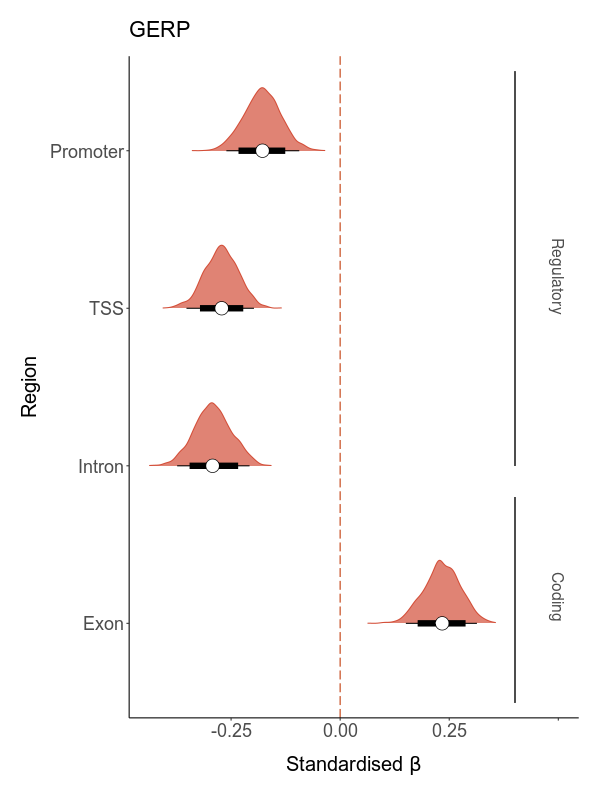
\includegraphics[keepaspectratio]{qmd/../plots/main/fig_2c.png}}

}

\caption{Results per genomic region GERP}

\end{figure}%%
\begin{figure}[H]

{\centering \pandocbounded{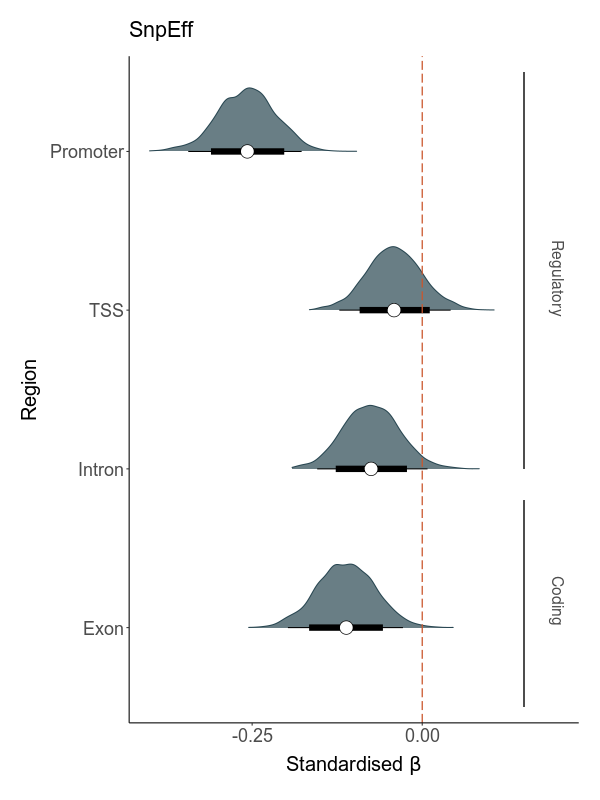
\includegraphics[keepaspectratio]{qmd/../plots/main/fig_2d.png}}

}

\caption{Results per genomic region SnpEff}

\end{figure}%

\begin{Shaded}
\begin{Highlighting}[]
\FunctionTok{library}\NormalTok{(readxl); }\FunctionTok{library}\NormalTok{(dplyr); }\FunctionTok{library}\NormalTok{(kableExtra)}
\NormalTok{gerp }\OtherTok{\textless{}{-}} \FunctionTok{read.csv}\NormalTok{(}\StringTok{"../output/models/intervals/regions\_gerp45.csv"}\NormalTok{)}
\NormalTok{gerp }\SpecialCharTok{\%\textgreater{}\%} \FunctionTok{kbl}\NormalTok{() }
\end{Highlighting}
\end{Shaded}

\begin{tabular}[t]{l|r|r|l|r|r|r|r|r|l}
\hline
parameter & outer\_width & inner\_width & point\_est & ll & l & m & h & hh & region\\
\hline
b\_scaletotal\_load & 0.95 & 0.8 & median & -0.26 & -0.23 & -0.18 & -0.13 & -0.09 & Promoter\\
\hline
b\_scaletotal\_load & 0.95 & 0.8 & median & -0.35 & -0.32 & -0.27 & -0.22 & -0.20 & TSS\\
\hline
b\_scaletotal\_load & 0.95 & 0.8 & median & -0.37 & -0.35 & -0.29 & -0.23 & -0.21 & Intron\\
\hline
b\_scaletotal\_load & 0.95 & 0.8 & median & 0.15 & 0.18 & 0.23 & 0.29 & 0.31 & Exon\\
\hline
\end{tabular}

\begin{Shaded}
\begin{Highlighting}[]
\NormalTok{high }\OtherTok{\textless{}{-}} \FunctionTok{read.csv}\NormalTok{(}\StringTok{"../output/models/intervals/regions\_high.csv"}\NormalTok{)}
\NormalTok{high }\SpecialCharTok{\%\textgreater{}\%} \FunctionTok{kbl}\NormalTok{()}
\end{Highlighting}
\end{Shaded}

\begin{tabular}[t]{l|r|r|l|r|r|r|r|r|l}
\hline
parameter & outer\_width & inner\_width & point\_est & ll & l & m & h & hh & region\\
\hline
b\_scaletotal\_load & 0.95 & 0.8 & median & -0.34 & -0.31 & -0.26 & -0.20 & -0.18 & Promoter\\
\hline
b\_scaletotal\_load & 0.95 & 0.8 & median & -0.12 & -0.09 & -0.04 & 0.01 & 0.04 & TSS\\
\hline
b\_scaletotal\_load & 0.95 & 0.8 & median & -0.15 & -0.13 & -0.08 & -0.02 & 0.01 & Intron\\
\hline
b\_scaletotal\_load & 0.95 & 0.8 & median & -0.20 & -0.17 & -0.11 & -0.06 & -0.03 & Exon\\
\hline
\end{tabular}

These results indicate that regulatory regions, especially promoter
regions (SnpEff) are very important!

\bookmarksetup{startatroot}

\chapter{Load per biological process}\label{load-per-biological-process}

\section{Introduction}\label{introduction-6}

Deleterious mutations that disrupt certain biological processes might
affect LMS more negatively than in others. To test if there are certain
biological processes where deleterious mutations have negative fitness
effects, we hypothesized six processes and used gene ontology
annotations. We used
\href{http://amigo.geneontology.org/amigo\%5D}{Amigo} to extract
deleterious mutations associated with the GO terms: androgen metabolism,
cellular respiration, developmental growth, immunity, muslce tissue
development and response to oxidative stress. In the scripts below,
you'll see how we calculate total load based on these GO terms.

\subsubsection{Subset mutations}\label{subset-mutations}

First, we subset the mutations located in genes associated with each GO
term, and calculate total load based on that subset. We also divide it
per genomic region (promoter, intron, exon). We work with lists to
iterate the process with ease by looping over the list items.

\begin{Shaded}
\begin{Highlighting}[]
\DocumentationTok{\#\#\#\# load packages \#\#\#\#}
\NormalTok{pacman}\SpecialCharTok{::}\FunctionTok{p\_load}\NormalTok{(BiocManager, rtracklayer, GenomicFeatures, BiocGenerics, data.table, tidyverse, genomation, GenomicRanges, tibble)}

\DocumentationTok{\#\#\#\# load the list of genes per GO term \#\#\#\#}
\NormalTok{files }\OtherTok{\textless{}{-}} \FunctionTok{list.files}\NormalTok{(}\AttributeTok{path =} \StringTok{"data/gene\_lists\_go"}\NormalTok{, }\AttributeTok{pattern =} \StringTok{"*.txt"}\NormalTok{, }\AttributeTok{full.names =}\NormalTok{ T)}

\NormalTok{list }\OtherTok{\textless{}{-}} \FunctionTok{list}\NormalTok{()}
\ControlFlowTok{for}\NormalTok{ (i }\ControlFlowTok{in} \DecValTok{1}\SpecialCharTok{:}\FunctionTok{length}\NormalTok{(files))\{}
\NormalTok{  data }\OtherTok{\textless{}{-}} \FunctionTok{fread}\NormalTok{(files[i])}
\NormalTok{  list[[i]] }\OtherTok{\textless{}{-}}\NormalTok{ data}
\NormalTok{\}}

\FunctionTok{names}\NormalTok{(list) }\OtherTok{\textless{}{-}} \FunctionTok{gsub}\NormalTok{(}\StringTok{"data/gene\_lists\_go/|.txt"}\NormalTok{, }\StringTok{""}\NormalTok{, files)}

\DocumentationTok{\#\#\#\# extract only the unique gene names per GO term \#\#\#\#}
\ControlFlowTok{for}\NormalTok{ (i }\ControlFlowTok{in} \DecValTok{1}\SpecialCharTok{:}\FunctionTok{length}\NormalTok{(list))\{}
\NormalTok{  list[[i]] }\OtherTok{\textless{}{-}}\NormalTok{ list[[i]] }\SpecialCharTok{\%\textgreater{}\%}\NormalTok{ dplyr}\SpecialCharTok{::}\FunctionTok{select}\NormalTok{(}\StringTok{\textasciigrave{}}\AttributeTok{V1}\StringTok{\textasciigrave{}}\NormalTok{) }\SpecialCharTok{\%\textgreater{}\%}
    \FunctionTok{mutate}\NormalTok{(}\AttributeTok{go\_term =} \FunctionTok{names}\NormalTok{(list[i])) }\SpecialCharTok{\%\textgreater{}\%}
\NormalTok{    dplyr}\SpecialCharTok{::}\FunctionTok{rename}\NormalTok{(}\AttributeTok{gene\_id =} \StringTok{\textasciigrave{}}\AttributeTok{V1}\StringTok{\textasciigrave{}}\NormalTok{) }\SpecialCharTok{\%\textgreater{}\%} \FunctionTok{unique}\NormalTok{() }\SpecialCharTok{\%\textgreater{}\%}
    \FunctionTok{mutate}\NormalTok{(}\AttributeTok{gene\_id =} \FunctionTok{toupper}\NormalTok{(gene\_id))}
\NormalTok{\}}

\DocumentationTok{\#\#\#\# GERP \#\#\#\#}
\DocumentationTok{\#\#\#\# import gerp data \#\#\#\#}
\FunctionTok{load}\NormalTok{(}\StringTok{"output/load/gerp/gerp\_over4.RData"}\NormalTok{)}
\NormalTok{gerp}\SpecialCharTok{$}\NormalTok{chr }\OtherTok{\textless{}{-}} \FunctionTok{gsub}\NormalTok{(}\StringTok{";"}\NormalTok{, }\StringTok{"\_\_"}\NormalTok{, gerp}\SpecialCharTok{$}\NormalTok{chr)}
\NormalTok{gerp}\SpecialCharTok{$}\NormalTok{chr }\OtherTok{\textless{}{-}} \FunctionTok{gsub}\NormalTok{(}\StringTok{"="}\NormalTok{, }\StringTok{"\_"}\NormalTok{, gerp}\SpecialCharTok{$}\NormalTok{chr)}
\NormalTok{gerp}\SpecialCharTok{$}\NormalTok{chr\_pos }\OtherTok{\textless{}{-}} \FunctionTok{paste0}\NormalTok{(gerp}\SpecialCharTok{$}\NormalTok{chr, }\StringTok{"\_"}\NormalTok{, gerp}\SpecialCharTok{$}\NormalTok{pos)}

\CommentTok{\# extract only the positions for annotation}
\NormalTok{gerp\_snps }\OtherTok{\textless{}{-}}\NormalTok{ gerp }\SpecialCharTok{\%\textgreater{}\%}\NormalTok{ dplyr}\SpecialCharTok{::}\FunctionTok{select}\NormalTok{(chr, pos)}
\NormalTok{gerp\_snps}\SpecialCharTok{$}\NormalTok{end }\OtherTok{\textless{}{-}}\NormalTok{ gerp\_snps}\SpecialCharTok{$}\NormalTok{pos}
\NormalTok{gerp\_snps}\SpecialCharTok{$}\NormalTok{start }\OtherTok{\textless{}{-}}\NormalTok{ gerp\_snps}\SpecialCharTok{$}\NormalTok{pos}
\NormalTok{gerp\_gr }\OtherTok{\textless{}{-}} \FunctionTok{as}\NormalTok{(gerp\_snps, }\StringTok{"GRanges"}\NormalTok{)}

\DocumentationTok{\#\#\#\# import gene regions \#\#\#\#}

\DocumentationTok{\#\#\# load annotation data \#\#\#\#}
\NormalTok{annotation\_dir }\OtherTok{\textless{}{-}} \StringTok{"data/genomic/annotation"}

\NormalTok{promoter}\OtherTok{=}\FunctionTok{unique}\NormalTok{(}\FunctionTok{gffToGRanges}\NormalTok{(}\FunctionTok{paste0}\NormalTok{(annotation\_dir, }\StringTok{"/promoters.gff3"}\NormalTok{)))}
\NormalTok{exons\_gene}\OtherTok{=}\FunctionTok{unique}\NormalTok{(}\FunctionTok{gffToGRanges}\NormalTok{(}\FunctionTok{paste0}\NormalTok{(annotation\_dir, }\StringTok{"/exons\_gene.gff3"}\NormalTok{)))}
\NormalTok{introns}\OtherTok{=}\FunctionTok{unique}\NormalTok{(}\FunctionTok{gffToGRanges}\NormalTok{(}\FunctionTok{paste0}\NormalTok{(annotation\_dir, }\StringTok{"/introns\_transcripts.gff3"}\NormalTok{)))}

\DocumentationTok{\#\#\#\# annotate gerp mutations \#\#\#\#}

\NormalTok{gerp\_promoter }\OtherTok{\textless{}{-}} \FunctionTok{as.data.frame}\NormalTok{(}\FunctionTok{mergeByOverlaps}\NormalTok{(gerp\_gr, promoter)) }\SpecialCharTok{\%\textgreater{}\%}
  \FunctionTok{add\_column}\NormalTok{(}\StringTok{"region\_promoter"} \OtherTok{=} \DecValTok{1}\NormalTok{) }\SpecialCharTok{\%\textgreater{}\%} \FunctionTok{unique}\NormalTok{() }\SpecialCharTok{\%\textgreater{}\%}\NormalTok{ dplyr}\SpecialCharTok{::}\FunctionTok{select}\NormalTok{(}\FunctionTok{c}\NormalTok{(}\StringTok{\textasciigrave{}}\AttributeTok{gerp\_gr.seqnames}\StringTok{\textasciigrave{}}\NormalTok{, pos, region\_promoter,ID)) }\SpecialCharTok{\%\textgreater{}\%}\NormalTok{ dplyr}\SpecialCharTok{::}\FunctionTok{rename}\NormalTok{(}\AttributeTok{chr =}\NormalTok{ gerp\_gr.seqnames)}

\NormalTok{gerp\_exons }\OtherTok{\textless{}{-}} \FunctionTok{as.data.frame}\NormalTok{(}\FunctionTok{mergeByOverlaps}\NormalTok{(gerp\_gr, exons\_gene))}\SpecialCharTok{\%\textgreater{}\%}
  \FunctionTok{add\_column}\NormalTok{(}\StringTok{"region\_exon"} \OtherTok{=} \DecValTok{1}\NormalTok{) }\SpecialCharTok{\%\textgreater{}\%} \FunctionTok{unique}\NormalTok{() }\SpecialCharTok{\%\textgreater{}\%}\NormalTok{ dplyr}\SpecialCharTok{::}\FunctionTok{select}\NormalTok{(}\FunctionTok{c}\NormalTok{(gerp\_gr.seqnames, pos, region\_exon,ID)) }\SpecialCharTok{\%\textgreater{}\%}\NormalTok{ dplyr}\SpecialCharTok{::}\FunctionTok{rename}\NormalTok{(}\AttributeTok{chr =}\NormalTok{ gerp\_gr.seqnames)}

\NormalTok{gerp\_intron }\OtherTok{\textless{}{-}} \FunctionTok{as.data.frame}\NormalTok{(}\FunctionTok{mergeByOverlaps}\NormalTok{(gerp\_gr, introns))}\SpecialCharTok{\%\textgreater{}\%}
  \FunctionTok{add\_column}\NormalTok{(}\StringTok{"region\_intron"} \OtherTok{=} \StringTok{"1"}\NormalTok{) }\SpecialCharTok{\%\textgreater{}\%} \FunctionTok{unique}\NormalTok{() }\SpecialCharTok{\%\textgreater{}\%}\NormalTok{ dplyr}\SpecialCharTok{::}\FunctionTok{select}\NormalTok{(}\FunctionTok{c}\NormalTok{(gerp\_gr.seqnames, pos, region\_intron,ID)) }\SpecialCharTok{\%\textgreater{}\%}\NormalTok{ dplyr}\SpecialCharTok{::}\FunctionTok{rename}\NormalTok{(}\AttributeTok{chr =}\NormalTok{ gerp\_gr.seqnames)}


\NormalTok{gerp\_list }\OtherTok{\textless{}{-}} \FunctionTok{list}\NormalTok{(gerp\_promoter, gerp\_exons, gerp\_intron)}

\DocumentationTok{\#\#\#\# merge with \textquotesingle{}similar to\textquotesingle{} column to get gene IDs \#\#\#\#}
\NormalTok{lookup }\OtherTok{\textless{}{-}} \FunctionTok{fread}\NormalTok{(}\StringTok{"../grouse{-}annotation/data/lookup\_ANN\_gene\_id.txt"}\NormalTok{)}
\FunctionTok{names}\NormalTok{(lookup) }\OtherTok{\textless{}{-}} \FunctionTok{c}\NormalTok{(}\StringTok{"ann"}\NormalTok{, }\StringTok{"gene\_id"}\NormalTok{)}

\ControlFlowTok{for}\NormalTok{ (i }\ControlFlowTok{in} \DecValTok{1}\SpecialCharTok{:}\FunctionTok{length}\NormalTok{(gerp\_list))\{}
\NormalTok{  gerp\_list[[i]] }\OtherTok{\textless{}{-}} \FunctionTok{left\_join}\NormalTok{(gerp\_list[[i]], lookup, }\AttributeTok{by =} \FunctionTok{c}\NormalTok{(}\StringTok{"ID"} \OtherTok{=} \StringTok{"ann"}\NormalTok{))}
  \FunctionTok{names}\NormalTok{(gerp\_list[[i]])[}\DecValTok{4}\NormalTok{] }\OtherTok{\textless{}{-}} \FunctionTok{c}\NormalTok{(}\StringTok{"ann"}\NormalTok{)}
\NormalTok{  gerp\_list[[i]]}\SpecialCharTok{$}\NormalTok{gene\_id }\OtherTok{\textless{}{-}} \FunctionTok{toupper}\NormalTok{(gerp\_list[[i]]}\SpecialCharTok{$}\NormalTok{gene\_id)}
\NormalTok{\}}

\DocumentationTok{\#\#\#\# extract snps per GO term \#\#\#\#}

\NormalTok{go\_snps\_promo }\OtherTok{\textless{}{-}} \FunctionTok{list}\NormalTok{()}
\ControlFlowTok{for}\NormalTok{ (i }\ControlFlowTok{in} \DecValTok{1}\SpecialCharTok{:}\FunctionTok{length}\NormalTok{(list))\{}
\NormalTok{  overlap }\OtherTok{\textless{}{-}} \FunctionTok{subset}\NormalTok{(gerp\_list[[}\DecValTok{1}\NormalTok{]], gene\_id }\SpecialCharTok{\%in\%}\NormalTok{ list[[i]]}\SpecialCharTok{$}\NormalTok{gene\_id)}
\NormalTok{  go\_snps\_promo[[i]] }\OtherTok{\textless{}{-}}\NormalTok{ overlap\}}

\NormalTok{go\_snps\_exon }\OtherTok{\textless{}{-}} \FunctionTok{list}\NormalTok{()}
\ControlFlowTok{for}\NormalTok{ (i }\ControlFlowTok{in} \DecValTok{1}\SpecialCharTok{:}\FunctionTok{length}\NormalTok{(list))\{}
\NormalTok{  overlap }\OtherTok{\textless{}{-}} \FunctionTok{subset}\NormalTok{(gerp\_list[[}\DecValTok{2}\NormalTok{]], gene\_id }\SpecialCharTok{\%in\%}\NormalTok{ list[[i]]}\SpecialCharTok{$}\NormalTok{gene\_id)}
\NormalTok{  go\_snps\_exon[[i]] }\OtherTok{\textless{}{-}}\NormalTok{ overlap\}}

\NormalTok{go\_snps\_intron }\OtherTok{\textless{}{-}} \FunctionTok{list}\NormalTok{()}
\ControlFlowTok{for}\NormalTok{ (i }\ControlFlowTok{in} \DecValTok{1}\SpecialCharTok{:}\FunctionTok{length}\NormalTok{(list))\{}
\NormalTok{  overlap }\OtherTok{\textless{}{-}} \FunctionTok{subset}\NormalTok{(gerp\_list[[}\DecValTok{3}\NormalTok{]], gene\_id }\SpecialCharTok{\%in\%}\NormalTok{ list[[i]]}\SpecialCharTok{$}\NormalTok{gene\_id)}
\NormalTok{  go\_snps\_intron[[i]] }\OtherTok{\textless{}{-}}\NormalTok{ overlap\}}

\CommentTok{\# name}
\FunctionTok{names}\NormalTok{(go\_snps\_promo) }\OtherTok{\textless{}{-}} \FunctionTok{names}\NormalTok{(list)}
\FunctionTok{names}\NormalTok{(go\_snps\_exon) }\OtherTok{\textless{}{-}} \FunctionTok{names}\NormalTok{(list)}
\FunctionTok{names}\NormalTok{(go\_snps\_intron) }\OtherTok{\textless{}{-}} \FunctionTok{names}\NormalTok{(list)}

\NormalTok{summary\_snps\_per\_go }\OtherTok{\textless{}{-}} \FunctionTok{data.frame}\NormalTok{()}
\ControlFlowTok{for}\NormalTok{ (i }\ControlFlowTok{in} \DecValTok{1}\SpecialCharTok{:}\FunctionTok{length}\NormalTok{(list))\{}
\NormalTok{  snps\_go }\OtherTok{\textless{}{-}} \FunctionTok{data.frame}\NormalTok{(}\AttributeTok{go =} \FunctionTok{names}\NormalTok{(list[i]),}
                        \AttributeTok{snps\_promo =} \FunctionTok{nrow}\NormalTok{(}\FunctionTok{subset}\NormalTok{(go\_snps\_promo[[i]], region\_promoter }\SpecialCharTok{==} \DecValTok{1}\NormalTok{)),}
                        \AttributeTok{snps\_exon =} \FunctionTok{nrow}\NormalTok{(}\FunctionTok{subset}\NormalTok{(go\_snps\_exon[[i]], region\_exon }\SpecialCharTok{==} \DecValTok{1}\NormalTok{)),}
                        \AttributeTok{snps\_intron =} \FunctionTok{nrow}\NormalTok{(}\FunctionTok{subset}\NormalTok{(go\_snps\_intron[[i]], region\_intron }\SpecialCharTok{==} \DecValTok{1}\NormalTok{)),}
                        \AttributeTok{og\_genes\_total =} \FunctionTok{nrow}\NormalTok{(list[[i]]))}
\NormalTok{  summary\_snps\_per\_go }\OtherTok{\textless{}{-}} \FunctionTok{rbind}\NormalTok{(summary\_snps\_per\_go, snps\_go)}
\NormalTok{\}}

\CommentTok{\# how many genes}
\NormalTok{genes\_n }\OtherTok{\textless{}{-}} \FunctionTok{data.frame}\NormalTok{()}
\ControlFlowTok{for}\NormalTok{ (i }\ControlFlowTok{in} \DecValTok{1}\SpecialCharTok{:}\FunctionTok{length}\NormalTok{(list))\{}
\NormalTok{  promo }\OtherTok{\textless{}{-}} \FunctionTok{subset}\NormalTok{(go\_snps\_promo[[i]], region\_promoter }\SpecialCharTok{==} \DecValTok{1}\NormalTok{)}
\NormalTok{  exon }\OtherTok{\textless{}{-}} \FunctionTok{subset}\NormalTok{(go\_snps\_exon[[i]], region\_exon }\SpecialCharTok{==} \DecValTok{1}\NormalTok{)}
\NormalTok{  intron }\OtherTok{\textless{}{-}} \FunctionTok{subset}\NormalTok{(go\_snps\_intron[[i]], region\_intron }\SpecialCharTok{==} \DecValTok{1}\NormalTok{)}
\NormalTok{  genes }\OtherTok{\textless{}{-}} \FunctionTok{unique}\NormalTok{(}\FunctionTok{c}\NormalTok{(promo}\SpecialCharTok{$}\NormalTok{gene\_id, exon}\SpecialCharTok{$}\NormalTok{gene\_id, intron}\SpecialCharTok{$}\NormalTok{gene\_id))}
\NormalTok{  genes\_go }\OtherTok{\textless{}{-}} \FunctionTok{data.frame}\NormalTok{(}\AttributeTok{go =} \FunctionTok{names}\NormalTok{(list[i]),}
                        \AttributeTok{n\_genes =} \FunctionTok{length}\NormalTok{(genes))}
\NormalTok{  genes\_n }\OtherTok{\textless{}{-}} \FunctionTok{rbind}\NormalTok{(genes\_n, genes\_go)}
\NormalTok{\}}

\FunctionTok{write\_tsv}\NormalTok{(genes\_n, }\AttributeTok{file =} \StringTok{"output/biological\_pathways/n\_genes\_gerp\_per\_go.tsv"}\NormalTok{)}
\CommentTok{\#note: there are snps for every go term!}

\DocumentationTok{\#\#\#\# extract genotypes per GO term \#\#\#\#}
\CommentTok{\#promo}
\NormalTok{genotypes\_go\_promo }\OtherTok{\textless{}{-}} \FunctionTok{list}\NormalTok{()}

\ControlFlowTok{for}\NormalTok{ (i }\ControlFlowTok{in} \DecValTok{1}\SpecialCharTok{:}\FunctionTok{length}\NormalTok{(go\_snps\_promo))\{}
\NormalTok{  go\_snps\_promo[[i]]}\SpecialCharTok{$}\NormalTok{chr\_pos }\OtherTok{\textless{}{-}} \FunctionTok{paste0}\NormalTok{(go\_snps\_promo[[i]]}\SpecialCharTok{$}\NormalTok{chr, }\StringTok{"\_"}\NormalTok{, go\_snps\_promo[[i]]}\SpecialCharTok{$}\NormalTok{pos)}
\NormalTok{  geno }\OtherTok{\textless{}{-}} \FunctionTok{subset}\NormalTok{(gerp, chr\_pos }\SpecialCharTok{\%in\%}\NormalTok{ go\_snps\_promo[[i]]}\SpecialCharTok{$}\NormalTok{chr\_pos)}
\NormalTok{  geno}\SpecialCharTok{$}\NormalTok{chr\_pos }\OtherTok{\textless{}{-}} \ConstantTok{NULL}
\NormalTok{  genotypes\_go\_promo[[i]] }\OtherTok{\textless{}{-}}\NormalTok{ geno}
\NormalTok{\}}
\FunctionTok{names}\NormalTok{(genotypes\_go\_promo) }\OtherTok{\textless{}{-}} \FunctionTok{names}\NormalTok{(list)}

\CommentTok{\#exon}
\NormalTok{genotypes\_go\_exon }\OtherTok{\textless{}{-}} \FunctionTok{list}\NormalTok{()}

\ControlFlowTok{for}\NormalTok{ (i }\ControlFlowTok{in} \DecValTok{1}\SpecialCharTok{:}\FunctionTok{length}\NormalTok{(go\_snps\_exon))\{}
\NormalTok{  go\_snps\_exon[[i]]}\SpecialCharTok{$}\NormalTok{chr\_pos }\OtherTok{\textless{}{-}} \FunctionTok{paste0}\NormalTok{(go\_snps\_exon[[i]]}\SpecialCharTok{$}\NormalTok{chr, }\StringTok{"\_"}\NormalTok{, go\_snps\_exon[[i]]}\SpecialCharTok{$}\NormalTok{pos)}
\NormalTok{  geno }\OtherTok{\textless{}{-}} \FunctionTok{subset}\NormalTok{(gerp, chr\_pos }\SpecialCharTok{\%in\%}\NormalTok{ go\_snps\_exon[[i]]}\SpecialCharTok{$}\NormalTok{chr\_pos)}
\NormalTok{  geno}\SpecialCharTok{$}\NormalTok{chr\_pos }\OtherTok{\textless{}{-}} \ConstantTok{NULL}
\NormalTok{  genotypes\_go\_exon[[i]] }\OtherTok{\textless{}{-}}\NormalTok{ geno}
\NormalTok{\}}
\FunctionTok{names}\NormalTok{(genotypes\_go\_exon) }\OtherTok{\textless{}{-}} \FunctionTok{names}\NormalTok{(list)}

\CommentTok{\#intron}
\NormalTok{genotypes\_go\_intron }\OtherTok{\textless{}{-}} \FunctionTok{list}\NormalTok{()}

\ControlFlowTok{for}\NormalTok{ (i }\ControlFlowTok{in} \DecValTok{1}\SpecialCharTok{:}\FunctionTok{length}\NormalTok{(go\_snps\_intron))\{}
\NormalTok{  go\_snps\_intron[[i]]}\SpecialCharTok{$}\NormalTok{chr\_pos }\OtherTok{\textless{}{-}} \FunctionTok{paste0}\NormalTok{(go\_snps\_intron[[i]]}\SpecialCharTok{$}\NormalTok{chr, }\StringTok{"\_"}\NormalTok{, go\_snps\_intron[[i]]}\SpecialCharTok{$}\NormalTok{pos)}
\NormalTok{  geno }\OtherTok{\textless{}{-}} \FunctionTok{subset}\NormalTok{(gerp, chr\_pos }\SpecialCharTok{\%in\%}\NormalTok{ go\_snps\_intron[[i]]}\SpecialCharTok{$}\NormalTok{chr\_pos)}
\NormalTok{  geno}\SpecialCharTok{$}\NormalTok{chr\_pos }\OtherTok{\textless{}{-}} \ConstantTok{NULL}
\NormalTok{  genotypes\_go\_intron[[i]] }\OtherTok{\textless{}{-}}\NormalTok{ geno}
\NormalTok{\}}
\FunctionTok{names}\NormalTok{(genotypes\_go\_intron) }\OtherTok{\textless{}{-}} \FunctionTok{names}\NormalTok{(list)}

\DocumentationTok{\#\#\#\# SnpEff \#\#\#\#}
\DocumentationTok{\#\#\#\# extract only the unique gene names per GO term \#\#\#\#}

\DocumentationTok{\#\#\#\# import snpeff data \#\#\#\#}
\FunctionTok{load}\NormalTok{(}\StringTok{"output/load/snpeff/snpeff\_high.RData"}\NormalTok{)}
\NormalTok{snpeff}\SpecialCharTok{$}\NormalTok{CHROM }\OtherTok{\textless{}{-}} \FunctionTok{gsub}\NormalTok{(}\StringTok{";"}\NormalTok{, }\StringTok{"\_\_"}\NormalTok{, snpeff}\SpecialCharTok{$}\NormalTok{CHROM)}
\NormalTok{snpeff}\SpecialCharTok{$}\NormalTok{CHROM }\OtherTok{\textless{}{-}} \FunctionTok{gsub}\NormalTok{(}\StringTok{"="}\NormalTok{, }\StringTok{"\_"}\NormalTok{, snpeff}\SpecialCharTok{$}\NormalTok{CHROM)}
\NormalTok{snpeff}\SpecialCharTok{$}\NormalTok{chr\_pos }\OtherTok{\textless{}{-}} \FunctionTok{paste0}\NormalTok{(snpeff}\SpecialCharTok{$}\NormalTok{CHROM, }\StringTok{"\_"}\NormalTok{, snpeff}\SpecialCharTok{$}\NormalTok{POS)}

\CommentTok{\# extract only the positions for annotation}
\NormalTok{snpeff\_snps }\OtherTok{\textless{}{-}}\NormalTok{ snpeff }\SpecialCharTok{\%\textgreater{}\%}\NormalTok{ dplyr}\SpecialCharTok{::}\FunctionTok{select}\NormalTok{(CHROM, POS)}
\NormalTok{snpeff\_snps}\SpecialCharTok{$}\NormalTok{end }\OtherTok{\textless{}{-}}\NormalTok{ snpeff\_snps}\SpecialCharTok{$}\NormalTok{POS}
\NormalTok{snpeff\_snps}\SpecialCharTok{$}\NormalTok{start }\OtherTok{\textless{}{-}}\NormalTok{ snpeff\_snps}\SpecialCharTok{$}\NormalTok{POS}
\NormalTok{snpeff\_gr }\OtherTok{\textless{}{-}} \FunctionTok{as}\NormalTok{(snpeff\_snps, }\StringTok{"GRanges"}\NormalTok{)}

\DocumentationTok{\#\#\#\# import gene regions \#\#\#\#}

\DocumentationTok{\#\#\#\# annotate snpeff mutations \#\#\#\#}
\NormalTok{snpeff\_promoter }\OtherTok{\textless{}{-}} \FunctionTok{mergeByOverlaps}\NormalTok{(snpeff\_gr, promoter)}
\NormalTok{snpeff\_promoter }\OtherTok{\textless{}{-}} \FunctionTok{as.data.frame}\NormalTok{(snpeff\_promoter}\SpecialCharTok{@}\NormalTok{listData)}
\NormalTok{snpeff\_promoter }\OtherTok{\textless{}{-}}\NormalTok{ snpeff\_promoter }\SpecialCharTok{\%\textgreater{}\%}
  \FunctionTok{add\_column}\NormalTok{(}\StringTok{"region\_promoter"} \OtherTok{=} \DecValTok{1}\NormalTok{) }\SpecialCharTok{\%\textgreater{}\%} \FunctionTok{unique}\NormalTok{() }\SpecialCharTok{\%\textgreater{}\%}\NormalTok{ dplyr}\SpecialCharTok{::}\FunctionTok{select}\NormalTok{(}\FunctionTok{c}\NormalTok{(}\StringTok{\textasciigrave{}}\AttributeTok{snpeff\_gr.seqnames}\StringTok{\textasciigrave{}}\NormalTok{, POS, region\_promoter,ID)) }\SpecialCharTok{\%\textgreater{}\%}\NormalTok{ dplyr}\SpecialCharTok{::}\FunctionTok{rename}\NormalTok{(}\AttributeTok{chr =}\NormalTok{ snpeff\_gr.seqnames)}

\NormalTok{snpeff\_exons }\OtherTok{\textless{}{-}} \FunctionTok{mergeByOverlaps}\NormalTok{(snpeff\_gr, exons\_gene)}
\NormalTok{snpeff\_exons }\OtherTok{\textless{}{-}} \FunctionTok{as.data.frame}\NormalTok{(snpeff\_exons}\SpecialCharTok{@}\NormalTok{listData)}
\NormalTok{snpeff\_exons }\OtherTok{\textless{}{-}}\NormalTok{ snpeff\_exons}\SpecialCharTok{\%\textgreater{}\%}
  \FunctionTok{add\_column}\NormalTok{(}\StringTok{"region\_exon"} \OtherTok{=} \DecValTok{1}\NormalTok{) }\SpecialCharTok{\%\textgreater{}\%} \FunctionTok{unique}\NormalTok{() }\SpecialCharTok{\%\textgreater{}\%}\NormalTok{ dplyr}\SpecialCharTok{::}\FunctionTok{select}\NormalTok{(}\FunctionTok{c}\NormalTok{(snpeff\_gr.seqnames, POS, region\_exon,ID)) }\SpecialCharTok{\%\textgreater{}\%}\NormalTok{ dplyr}\SpecialCharTok{::}\FunctionTok{rename}\NormalTok{(}\AttributeTok{chr =}\NormalTok{ snpeff\_gr.seqnames)}

\NormalTok{snpeff\_introns }\OtherTok{\textless{}{-}} \FunctionTok{mergeByOverlaps}\NormalTok{(snpeff\_gr, introns)}
\NormalTok{snpeff\_introns }\OtherTok{\textless{}{-}} \FunctionTok{as.data.frame}\NormalTok{(snpeff\_introns}\SpecialCharTok{@}\NormalTok{listData)}
\NormalTok{snpeff\_introns }\OtherTok{\textless{}{-}}\NormalTok{ snpeff\_introns}\SpecialCharTok{\%\textgreater{}\%}
  \FunctionTok{add\_column}\NormalTok{(}\StringTok{"region\_intron"} \OtherTok{=} \DecValTok{1}\NormalTok{) }\SpecialCharTok{\%\textgreater{}\%} \FunctionTok{unique}\NormalTok{() }\SpecialCharTok{\%\textgreater{}\%}\NormalTok{ dplyr}\SpecialCharTok{::}\FunctionTok{select}\NormalTok{(}\FunctionTok{c}\NormalTok{(snpeff\_gr.seqnames, POS, region\_intron,ID)) }\SpecialCharTok{\%\textgreater{}\%}\NormalTok{ dplyr}\SpecialCharTok{::}\FunctionTok{rename}\NormalTok{(}\AttributeTok{chr =}\NormalTok{ snpeff\_gr.seqnames)}

\NormalTok{snpeff\_list }\OtherTok{\textless{}{-}} \FunctionTok{list}\NormalTok{(snpeff\_promoter, snpeff\_exons, snpeff\_introns)}

\DocumentationTok{\#\#\#\# merge with \textquotesingle{}similar to\textquotesingle{} column to get gene IDs \#\#\#\#}
\NormalTok{lookup }\OtherTok{\textless{}{-}} \FunctionTok{fread}\NormalTok{(}\StringTok{"data/genomic/annotation/lookup\_ANN\_gene\_id.txt"}\NormalTok{)}
\FunctionTok{names}\NormalTok{(lookup) }\OtherTok{\textless{}{-}} \FunctionTok{c}\NormalTok{(}\StringTok{"ann"}\NormalTok{, }\StringTok{"gene\_id"}\NormalTok{)}

\ControlFlowTok{for}\NormalTok{ (i }\ControlFlowTok{in} \DecValTok{1}\SpecialCharTok{:}\FunctionTok{length}\NormalTok{(snpeff\_list))\{}
\NormalTok{  snpeff\_list[[i]] }\OtherTok{\textless{}{-}} \FunctionTok{left\_join}\NormalTok{(snpeff\_list[[i]], lookup, }\AttributeTok{by =} \FunctionTok{c}\NormalTok{(}\StringTok{"ID"} \OtherTok{=} \StringTok{"ann"}\NormalTok{))}
  \FunctionTok{names}\NormalTok{(snpeff\_list[[i]])[}\DecValTok{4}\NormalTok{] }\OtherTok{\textless{}{-}} \FunctionTok{c}\NormalTok{(}\StringTok{"ann"}\NormalTok{)}
\NormalTok{  snpeff\_list[[i]]}\SpecialCharTok{$}\NormalTok{gene\_id }\OtherTok{\textless{}{-}} \FunctionTok{toupper}\NormalTok{(snpeff\_list[[i]]}\SpecialCharTok{$}\NormalTok{gene\_id)}
\NormalTok{\}}

\DocumentationTok{\#\#\#\# extract snps per GO term \#\#\#\#}

\NormalTok{go\_snps\_promo\_snpeff }\OtherTok{\textless{}{-}} \FunctionTok{list}\NormalTok{()}
\ControlFlowTok{for}\NormalTok{ (i }\ControlFlowTok{in} \DecValTok{1}\SpecialCharTok{:}\FunctionTok{length}\NormalTok{(list))\{}
\NormalTok{  overlap }\OtherTok{\textless{}{-}} \FunctionTok{subset}\NormalTok{(snpeff\_list[[}\DecValTok{1}\NormalTok{]], gene\_id }\SpecialCharTok{\%in\%}\NormalTok{ list[[i]]}\SpecialCharTok{$}\NormalTok{gene\_id)}
\NormalTok{  go\_snps\_promo\_snpeff[[i]] }\OtherTok{\textless{}{-}}\NormalTok{ overlap\}}

\NormalTok{go\_snps\_exon\_snpeff }\OtherTok{\textless{}{-}} \FunctionTok{list}\NormalTok{()}
\ControlFlowTok{for}\NormalTok{ (i }\ControlFlowTok{in} \DecValTok{1}\SpecialCharTok{:}\FunctionTok{length}\NormalTok{(list))\{}
\NormalTok{  overlap }\OtherTok{\textless{}{-}} \FunctionTok{subset}\NormalTok{(snpeff\_list[[}\DecValTok{2}\NormalTok{]], gene\_id }\SpecialCharTok{\%in\%}\NormalTok{ list[[i]]}\SpecialCharTok{$}\NormalTok{gene\_id)}
\NormalTok{  go\_snps\_exon\_snpeff[[i]] }\OtherTok{\textless{}{-}}\NormalTok{ overlap\}}

\NormalTok{go\_snps\_intron\_snpeff }\OtherTok{\textless{}{-}} \FunctionTok{list}\NormalTok{()}
\ControlFlowTok{for}\NormalTok{ (i }\ControlFlowTok{in} \DecValTok{1}\SpecialCharTok{:}\FunctionTok{length}\NormalTok{(list))\{}
\NormalTok{  overlap }\OtherTok{\textless{}{-}} \FunctionTok{subset}\NormalTok{(snpeff\_list[[}\DecValTok{3}\NormalTok{]], gene\_id }\SpecialCharTok{\%in\%}\NormalTok{ list[[i]]}\SpecialCharTok{$}\NormalTok{gene\_id)}
\NormalTok{  go\_snps\_intron\_snpeff[[i]] }\OtherTok{\textless{}{-}}\NormalTok{ overlap\}}

\CommentTok{\# name}
\FunctionTok{names}\NormalTok{(go\_snps\_promo\_snpeff) }\OtherTok{\textless{}{-}} \FunctionTok{names}\NormalTok{(list)}
\FunctionTok{names}\NormalTok{(go\_snps\_exon\_snpeff) }\OtherTok{\textless{}{-}} \FunctionTok{names}\NormalTok{(list)}
\FunctionTok{names}\NormalTok{(go\_snps\_intron\_snpeff) }\OtherTok{\textless{}{-}} \FunctionTok{names}\NormalTok{(list)}

\NormalTok{summary\_snps\_per\_go }\OtherTok{\textless{}{-}} \FunctionTok{data.frame}\NormalTok{()}
\ControlFlowTok{for}\NormalTok{ (i }\ControlFlowTok{in} \DecValTok{1}\SpecialCharTok{:}\FunctionTok{length}\NormalTok{(list))\{}
\NormalTok{  snps\_go }\OtherTok{\textless{}{-}} \FunctionTok{data.frame}\NormalTok{(}\AttributeTok{go =} \FunctionTok{names}\NormalTok{(list[i]),}
                        \AttributeTok{snps\_promo =} \FunctionTok{nrow}\NormalTok{(}\FunctionTok{subset}\NormalTok{(go\_snps\_promo\_snpeff[[i]], region\_promoter }\SpecialCharTok{==} \DecValTok{1}\NormalTok{)),}
                        \AttributeTok{snps\_exon =} \FunctionTok{nrow}\NormalTok{(}\FunctionTok{subset}\NormalTok{(go\_snps\_exon\_snpeff[[i]], region\_exon }\SpecialCharTok{==} \DecValTok{1}\NormalTok{)),}
                        \AttributeTok{snps\_intron =} \FunctionTok{nrow}\NormalTok{(}\FunctionTok{subset}\NormalTok{(go\_snps\_intron\_snpeff[[i]], region\_intron }\SpecialCharTok{==} \DecValTok{1}\NormalTok{)),}
                        \AttributeTok{og\_genes\_total =} \FunctionTok{nrow}\NormalTok{(list[[i]]))}
\NormalTok{  summary\_snps\_per\_go }\OtherTok{\textless{}{-}} \FunctionTok{rbind}\NormalTok{(summary\_snps\_per\_go, snps\_go)}
\NormalTok{\}}

\NormalTok{genes\_n\_snpeff }\OtherTok{\textless{}{-}} \FunctionTok{data.frame}\NormalTok{()}
\ControlFlowTok{for}\NormalTok{ (i }\ControlFlowTok{in} \DecValTok{1}\SpecialCharTok{:}\FunctionTok{length}\NormalTok{(list))\{}
\NormalTok{  promo }\OtherTok{\textless{}{-}} \FunctionTok{subset}\NormalTok{(go\_snps\_promo\_snpeff[[i]], region\_promoter }\SpecialCharTok{==} \DecValTok{1}\NormalTok{)}
\NormalTok{  exon }\OtherTok{\textless{}{-}} \FunctionTok{subset}\NormalTok{(go\_snps\_exon\_snpeff[[i]], region\_exon }\SpecialCharTok{==} \DecValTok{1}\NormalTok{)}
\NormalTok{  intron }\OtherTok{\textless{}{-}} \FunctionTok{subset}\NormalTok{(go\_snps\_intron\_snpeff[[i]], region\_intron }\SpecialCharTok{==} \DecValTok{1}\NormalTok{)}
\NormalTok{  genes }\OtherTok{\textless{}{-}} \FunctionTok{unique}\NormalTok{(}\FunctionTok{c}\NormalTok{(promo}\SpecialCharTok{$}\NormalTok{gene\_id, exon}\SpecialCharTok{$}\NormalTok{gene\_id, intron}\SpecialCharTok{$}\NormalTok{gene\_id))}
\NormalTok{  genes\_go }\OtherTok{\textless{}{-}} \FunctionTok{data.frame}\NormalTok{(}\AttributeTok{go =} \FunctionTok{names}\NormalTok{(list[i]),}
                         \AttributeTok{n\_genes =} \FunctionTok{length}\NormalTok{(genes))}
\NormalTok{  genes\_n\_snpeff }\OtherTok{\textless{}{-}} \FunctionTok{rbind}\NormalTok{(genes\_n\_snpeff, genes\_go)}
\NormalTok{\}}

\FunctionTok{write\_tsv}\NormalTok{(genes\_n\_snpeff, }\AttributeTok{file =} \StringTok{"output/biological\_pathways/n\_genes\_snpeff\_per\_go.tsv"}\NormalTok{)}

\CommentTok{\#note: there are snps for every go term!}

\DocumentationTok{\#\#\#\# extract genotypes per GO term \#\#\#\#}
\CommentTok{\#only select those with \textgreater{}10 snps}
\NormalTok{go\_snps\_promo\_snpeff }\OtherTok{\textless{}{-}}\NormalTok{ go\_snps\_promo\_snpeff[}\FunctionTok{c}\NormalTok{(}\DecValTok{2}\NormalTok{,}\DecValTok{4}\SpecialCharTok{:}\DecValTok{9}\NormalTok{)]}
\NormalTok{go\_snps\_exon\_snpeff }\OtherTok{\textless{}{-}}\NormalTok{ go\_snps\_exon\_snpeff[}\FunctionTok{c}\NormalTok{(}\DecValTok{2}\NormalTok{,}\DecValTok{4}\SpecialCharTok{:}\DecValTok{9}\NormalTok{)]}
\NormalTok{go\_snps\_intron\_snpeff }\OtherTok{\textless{}{-}}\NormalTok{ go\_snps\_intron\_snpeff[}\FunctionTok{c}\NormalTok{(}\DecValTok{2}\NormalTok{,}\DecValTok{4}\SpecialCharTok{:}\DecValTok{9}\NormalTok{)]}

\CommentTok{\#promo}
\NormalTok{genotypes\_go\_promo\_snpeff }\OtherTok{\textless{}{-}} \FunctionTok{list}\NormalTok{()}

\ControlFlowTok{for}\NormalTok{ (i }\ControlFlowTok{in} \DecValTok{1}\SpecialCharTok{:}\FunctionTok{length}\NormalTok{(go\_snps\_promo\_snpeff))\{}
\NormalTok{  go\_snps\_promo\_snpeff[[i]]}\SpecialCharTok{$}\NormalTok{chr\_pos }\OtherTok{\textless{}{-}} \FunctionTok{paste0}\NormalTok{(go\_snps\_promo\_snpeff[[i]]}\SpecialCharTok{$}\NormalTok{chr, }\StringTok{"\_"}\NormalTok{, go\_snps\_promo\_snpeff[[i]]}\SpecialCharTok{$}\NormalTok{POS)}
\NormalTok{  geno }\OtherTok{\textless{}{-}} \FunctionTok{subset}\NormalTok{(snpeff, chr\_pos }\SpecialCharTok{\%in\%}\NormalTok{ go\_snps\_promo\_snpeff[[i]]}\SpecialCharTok{$}\NormalTok{chr\_pos)}
\NormalTok{  geno}\SpecialCharTok{$}\NormalTok{chr\_pos }\OtherTok{\textless{}{-}} \ConstantTok{NULL}
\NormalTok{  genotypes\_go\_promo\_snpeff[[i]] }\OtherTok{\textless{}{-}}\NormalTok{ geno}
\NormalTok{\}}

\FunctionTok{names}\NormalTok{(genotypes\_go\_promo\_snpeff) }\OtherTok{\textless{}{-}} \FunctionTok{names}\NormalTok{(go\_snps\_promo\_snpeff)}

\CommentTok{\#exon}
\NormalTok{genotypes\_go\_exon\_snpeff }\OtherTok{\textless{}{-}} \FunctionTok{list}\NormalTok{()}

\ControlFlowTok{for}\NormalTok{ (i }\ControlFlowTok{in} \DecValTok{1}\SpecialCharTok{:}\FunctionTok{length}\NormalTok{(go\_snps\_exon\_snpeff))\{}
\NormalTok{  go\_snps\_exon\_snpeff[[i]]}\SpecialCharTok{$}\NormalTok{chr\_pos }\OtherTok{\textless{}{-}} \FunctionTok{paste0}\NormalTok{(go\_snps\_exon\_snpeff[[i]]}\SpecialCharTok{$}\NormalTok{chr, }\StringTok{"\_"}\NormalTok{, go\_snps\_exon\_snpeff[[i]]}\SpecialCharTok{$}\NormalTok{POS)}
\NormalTok{  geno }\OtherTok{\textless{}{-}} \FunctionTok{subset}\NormalTok{(snpeff, chr\_pos }\SpecialCharTok{\%in\%}\NormalTok{ go\_snps\_exon\_snpeff[[i]]}\SpecialCharTok{$}\NormalTok{chr\_pos)}
\NormalTok{  geno}\SpecialCharTok{$}\NormalTok{chr\_pos }\OtherTok{\textless{}{-}} \ConstantTok{NULL}
\NormalTok{  genotypes\_go\_exon\_snpeff[[i]] }\OtherTok{\textless{}{-}}\NormalTok{ geno}
\NormalTok{\}}
\FunctionTok{names}\NormalTok{(genotypes\_go\_exon\_snpeff) }\OtherTok{\textless{}{-}} \FunctionTok{names}\NormalTok{(go\_snps\_exon\_snpeff)}

\CommentTok{\#intron}
\NormalTok{genotypes\_go\_intron\_snpeff }\OtherTok{\textless{}{-}} \FunctionTok{list}\NormalTok{()}

\ControlFlowTok{for}\NormalTok{ (i }\ControlFlowTok{in} \DecValTok{1}\SpecialCharTok{:}\FunctionTok{length}\NormalTok{(go\_snps\_intron\_snpeff))\{}
\NormalTok{  go\_snps\_intron\_snpeff[[i]]}\SpecialCharTok{$}\NormalTok{chr\_pos }\OtherTok{\textless{}{-}} \FunctionTok{paste0}\NormalTok{(go\_snps\_intron\_snpeff[[i]]}\SpecialCharTok{$}\NormalTok{chr, }\StringTok{"\_"}\NormalTok{, go\_snps\_intron\_snpeff[[i]]}\SpecialCharTok{$}\NormalTok{POS)}
\NormalTok{  geno }\OtherTok{\textless{}{-}} \FunctionTok{subset}\NormalTok{(snpeff, chr\_pos }\SpecialCharTok{\%in\%}\NormalTok{ go\_snps\_intron\_snpeff[[i]]}\SpecialCharTok{$}\NormalTok{chr\_pos)}
\NormalTok{  geno}\SpecialCharTok{$}\NormalTok{chr\_pos }\OtherTok{\textless{}{-}} \ConstantTok{NULL}
\NormalTok{  genotypes\_go\_intron\_snpeff[[i]] }\OtherTok{\textless{}{-}}\NormalTok{ geno}
\NormalTok{\}}
\FunctionTok{names}\NormalTok{(genotypes\_go\_intron\_snpeff) }\OtherTok{\textless{}{-}} \FunctionTok{names}\NormalTok{(go\_snps\_intron\_snpeff)}
\end{Highlighting}
\end{Shaded}

\subsubsection{Calculate mutation load}\label{calculate-mutation-load-1}

Then, we calculate the total load based on these subsets, again for GERP
and SnpEff separately.

\begin{Shaded}
\begin{Highlighting}[]
\DocumentationTok{\#\#\#\# calculate mutation load based on mutations in each GO term \#\#\#\#}

\DocumentationTok{\#\#\# GERP}
\FunctionTok{source}\NormalTok{(}\StringTok{"scripts/7\_calculate\_load/function\_calculate\_load.R"}\NormalTok{)}

\NormalTok{loads }\OtherTok{\textless{}{-}} \FunctionTok{data.frame}\NormalTok{()}
\ControlFlowTok{for}\NormalTok{ (i }\ControlFlowTok{in} \DecValTok{1}\SpecialCharTok{:}\FunctionTok{length}\NormalTok{(list))\{}
  \CommentTok{\#promo}
\NormalTok{  load\_promo }\OtherTok{\textless{}{-}} \FunctionTok{calculate\_load\_gerp}\NormalTok{(}\FunctionTok{unique}\NormalTok{(genotypes\_go\_promo[[i]]), }\AttributeTok{loadtype =} \FunctionTok{names}\NormalTok{(genotypes\_go\_promo[i]), }\AttributeTok{output\_vcf =}\NormalTok{ F)}
\NormalTok{  load\_promo}\SpecialCharTok{$}\NormalTok{method }\OtherTok{\textless{}{-}} \StringTok{"gerp"}
\NormalTok{  load\_promo}\SpecialCharTok{$}\NormalTok{region }\OtherTok{=} \StringTok{"promo"}
\NormalTok{  loads }\OtherTok{\textless{}{-}} \FunctionTok{rbind}\NormalTok{(loads, load\_promo)}
  \CommentTok{\#exon}
\NormalTok{  load\_exon }\OtherTok{\textless{}{-}} \FunctionTok{calculate\_load\_gerp}\NormalTok{(genotypes\_go\_exon[[i]], }\AttributeTok{loadtype =} \FunctionTok{names}\NormalTok{(genotypes\_go\_exon[i]), }\AttributeTok{output\_vcf =}\NormalTok{ F)}
\NormalTok{  load\_exon}\SpecialCharTok{$}\NormalTok{method }\OtherTok{\textless{}{-}} \StringTok{"gerp"}
\NormalTok{  load\_exon}\SpecialCharTok{$}\NormalTok{region }\OtherTok{=} \StringTok{"exon"}
\NormalTok{  loads }\OtherTok{\textless{}{-}} \FunctionTok{rbind}\NormalTok{(loads, load\_exon)}
  \CommentTok{\#intron}
\NormalTok{  load\_intron }\OtherTok{\textless{}{-}} \FunctionTok{calculate\_load\_gerp}\NormalTok{(genotypes\_go\_intron[[i]], }\AttributeTok{loadtype =} \FunctionTok{names}\NormalTok{(genotypes\_go\_intron[i]), }\AttributeTok{output\_vcf =}\NormalTok{ F)}
\NormalTok{  load\_intron}\SpecialCharTok{$}\NormalTok{method }\OtherTok{\textless{}{-}} \StringTok{"gerp"}
\NormalTok{  load\_intron}\SpecialCharTok{$}\NormalTok{region }\OtherTok{=} \StringTok{"intron"}
\NormalTok{  loads }\OtherTok{\textless{}{-}} \FunctionTok{rbind}\NormalTok{(loads, load\_intron)}
\NormalTok{\}}

\DocumentationTok{\#\#\#\# SnpEff}
\NormalTok{loads\_snpeff }\OtherTok{\textless{}{-}} \FunctionTok{data.frame}\NormalTok{()}
\ControlFlowTok{for}\NormalTok{ (i }\ControlFlowTok{in} \DecValTok{1}\SpecialCharTok{:}\FunctionTok{length}\NormalTok{(genotypes\_go\_promo\_snpeff))\{}
  \CommentTok{\#promo}
\NormalTok{  load }\OtherTok{\textless{}{-}} \FunctionTok{calculate\_load\_snpeff}\NormalTok{(genotypes\_go\_promo\_snpeff[[i]], }\AttributeTok{loadtype =} \FunctionTok{names}\NormalTok{(genotypes\_go\_promo\_snpeff[i]), }\AttributeTok{output\_vcf =}\NormalTok{ F)}
\NormalTok{  load}\SpecialCharTok{$}\NormalTok{method }\OtherTok{\textless{}{-}} \StringTok{"snpeff"}
\NormalTok{  load}\SpecialCharTok{$}\NormalTok{region }\OtherTok{=} \StringTok{"promo"}
\NormalTok{  loads\_snpeff }\OtherTok{\textless{}{-}} \FunctionTok{rbind}\NormalTok{(loads\_snpeff, load)}
  \CommentTok{\#exon}
\NormalTok{  load }\OtherTok{\textless{}{-}} \FunctionTok{calculate\_load\_snpeff}\NormalTok{(genotypes\_go\_exon\_snpeff[[i]], }\AttributeTok{loadtype =} \FunctionTok{names}\NormalTok{(genotypes\_go\_exon\_snpeff[i]), }\AttributeTok{output\_vcf =}\NormalTok{ F)}
\NormalTok{  load}\SpecialCharTok{$}\NormalTok{method }\OtherTok{\textless{}{-}} \StringTok{"snpeff"}
\NormalTok{  load}\SpecialCharTok{$}\NormalTok{region }\OtherTok{=} \StringTok{"exon"}
\NormalTok{  loads\_snpeff }\OtherTok{\textless{}{-}} \FunctionTok{rbind}\NormalTok{(loads\_snpeff, load)}
  \CommentTok{\#intron}
\NormalTok{  load }\OtherTok{\textless{}{-}} \FunctionTok{calculate\_load\_snpeff}\NormalTok{(genotypes\_go\_intron\_snpeff[[i]], }\AttributeTok{loadtype =} \FunctionTok{names}\NormalTok{(genotypes\_go\_intron\_snpeff[i]), }\AttributeTok{output\_vcf =}\NormalTok{ F)}
\NormalTok{  load}\SpecialCharTok{$}\NormalTok{method }\OtherTok{\textless{}{-}} \StringTok{"snpeff"}
\NormalTok{  load}\SpecialCharTok{$}\NormalTok{region }\OtherTok{=} \StringTok{"intron"}
\NormalTok{  loads\_snpeff }\OtherTok{\textless{}{-}} \FunctionTok{rbind}\NormalTok{(loads\_snpeff, load)}
\NormalTok{\}}

\NormalTok{loads }\OtherTok{\textless{}{-}} \FunctionTok{rbind}\NormalTok{(loads, loads\_snpeff)}
\FunctionTok{save}\NormalTok{(loads, }\AttributeTok{file =} \StringTok{"output/biological\_pathways/loads\_per\_go\_term\_per\_region.RData"}\NormalTok{)}
\end{Highlighting}
\end{Shaded}

\subsection{Modelling}\label{modelling-1}

We then computed the exact same models as the total load models
presented before with the following model structure:

\texttt{LMS\ \textasciitilde{}\ scale(total\_load)\ +\ core\ +\ (1\textbar{}site)}

Where total load is not a measure taken from a subset of deleterious
mutations located within a specific genomic region and associated with a
certain subset of genes.

\subsection{Results}\label{results-4}

Below you find the posterior distributions:

\begin{figure}[H]

{\centering \pandocbounded{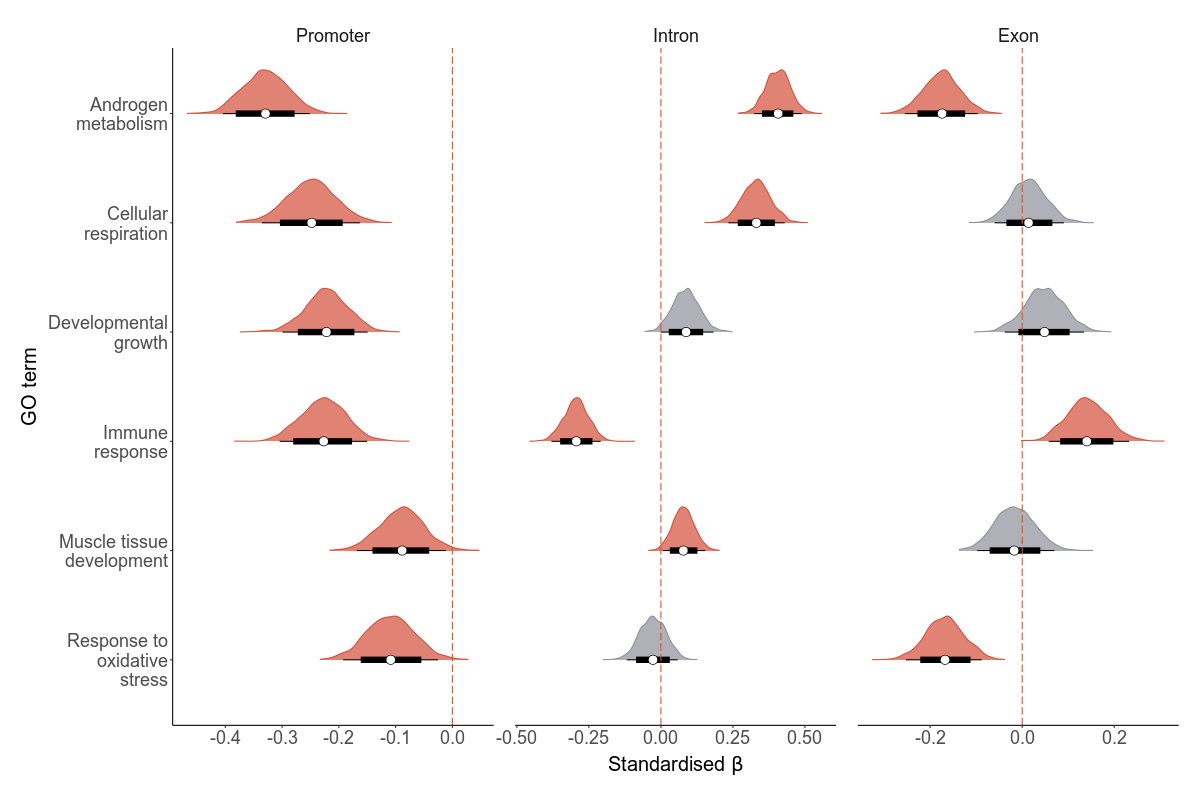
\includegraphics[keepaspectratio]{qmd/../plots/extended/extended_5_go_gerp.png}}

}

\caption{Results per genomic region per GO term for GERP}

\end{figure}%%
\begin{figure}[H]

{\centering \pandocbounded{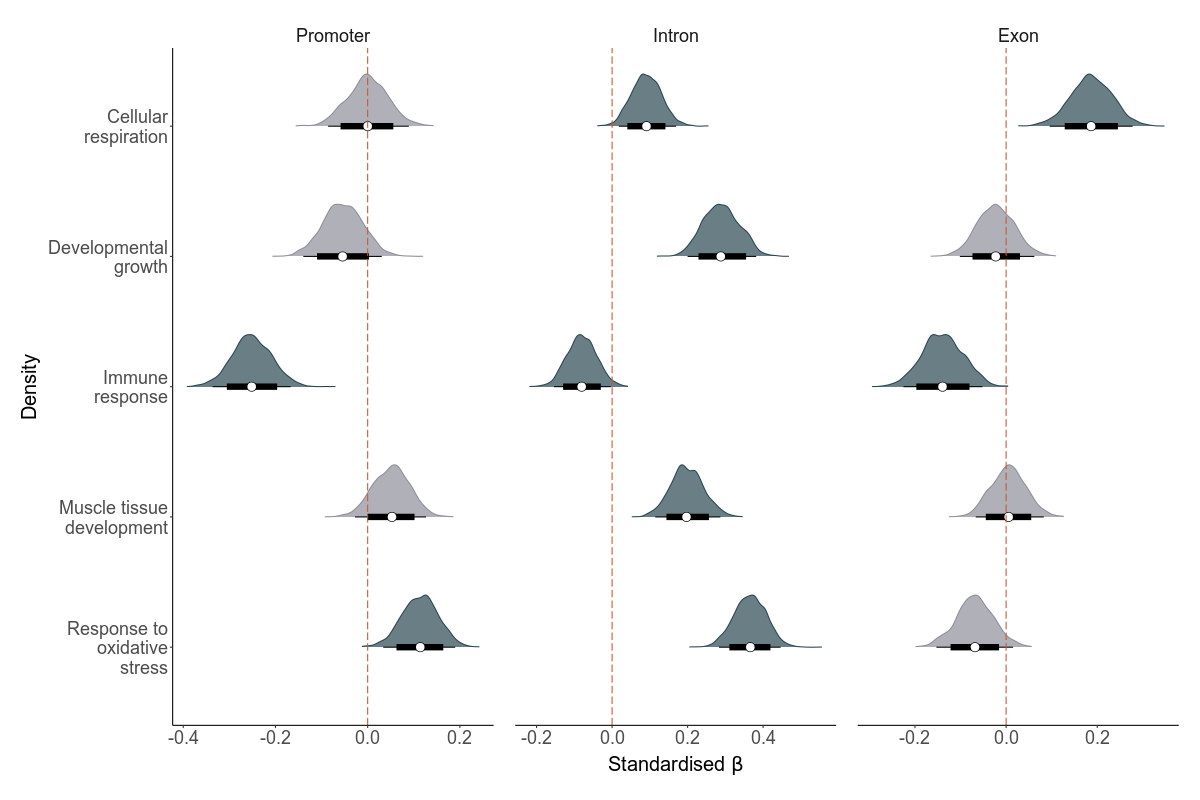
\includegraphics[keepaspectratio]{qmd/../plots/extended/extended_6_go_snpeff.png}}

}

\caption{Results per genomic region per GO term for SnpEff}

\end{figure}%

\begin{Shaded}
\begin{Highlighting}[]
\FunctionTok{library}\NormalTok{(data.table); }\FunctionTok{library}\NormalTok{(kableExtra)}
\NormalTok{gerp }\OtherTok{\textless{}{-}} \FunctionTok{fread}\NormalTok{(}\StringTok{"../output/biological\_pathways/intervals\_gerp.tsv"}\NormalTok{)}
\NormalTok{gerp }\SpecialCharTok{\%\textgreater{}\%} \FunctionTok{kbl}\NormalTok{() }
\end{Highlighting}
\end{Shaded}

\begin{tabular}[t]{l|l|l|r|l|l}
\hline
parameter & region & go & median & ci\_95 & ci\_80\\
\hline
b\_scaletotal\_load & Exon & Androgen metabolism & -0.17 & -0.25, -0.1 & -0.23, -0.12\\
\hline
b\_scaletotal\_load & Exon & Cellular respiration & 0.01 & -0.06, 0.09 & -0.03, 0.07\\
\hline
b\_scaletotal\_load & Exon & Developmental growth & 0.05 & -0.04, 0.13 & -0.01, 0.1\\
\hline
b\_scaletotal\_load & Exon & Immune response & 0.14 & 0.06, 0.23 & 0.08, 0.2\\
\hline
b\_scaletotal\_load & Exon & Muscle tissue development & -0.02 & -0.1, 0.07 & -0.07, 0.04\\
\hline
b\_scaletotal\_load & Exon & Response to oxidative stress & -0.17 & -0.25, -0.09 & -0.22, -0.11\\
\hline
b\_scaletotal\_load & Intron & Androgen metabolism & 0.41 & 0.32, 0.49 & 0.35, 0.46\\
\hline
b\_scaletotal\_load & Intron & Cellular respiration & 0.33 & 0.23, 0.43 & 0.27, 0.4\\
\hline
b\_scaletotal\_load & Intron & Developmental growth & 0.09 & 0, 0.18 & 0.03, 0.15\\
\hline
b\_scaletotal\_load & Intron & Immune response & -0.29 & -0.38, -0.21 & -0.35, -0.24\\
\hline
b\_scaletotal\_load & Intron & Muscle tissue development & 0.08 & 0.01, 0.15 & 0.03, 0.13\\
\hline
b\_scaletotal\_load & Intron & Response to oxidative stress & -0.03 & -0.12, 0.06 & -0.09, 0.03\\
\hline
b\_scaletotal\_load & Promoter & Androgen metabolism & -0.33 & -0.4, -0.25 & -0.38, -0.28\\
\hline
b\_scaletotal\_load & Promoter & Cellular respiration & -0.25 & -0.34, -0.16 & -0.3, -0.19\\
\hline
b\_scaletotal\_load & Promoter & Developmental growth & -0.22 & -0.3, -0.15 & -0.27, -0.17\\
\hline
b\_scaletotal\_load & Promoter & Immune response & -0.23 & -0.3, -0.15 & -0.28, -0.18\\
\hline
b\_scaletotal\_load & Promoter & Muscle tissue development & -0.09 & -0.17, -0.01 & -0.14, -0.04\\
\hline
b\_scaletotal\_load & Promoter & Response to oxidative stress & -0.11 & -0.19, -0.02 & -0.16, -0.05\\
\hline
\end{tabular}

\begin{Shaded}
\begin{Highlighting}[]
\NormalTok{high }\OtherTok{\textless{}{-}} \FunctionTok{fread}\NormalTok{(}\StringTok{"../output/biological\_pathways/intervals\_high.tsv"}\NormalTok{)}
\NormalTok{high }\SpecialCharTok{\%\textgreater{}\%} \FunctionTok{kbl}\NormalTok{()}
\end{Highlighting}
\end{Shaded}

\begin{tabular}[t]{l|l|l|r|l|l}
\hline
parameter & region & go & median & ci\_95 & ci\_80\\
\hline
b\_scaletotal\_load & Exon & Cellular respiration & 0.19 & 0.1, 0.28 & 0.13, 0.25\\
\hline
b\_scaletotal\_load & Exon & Developmental growth & -0.02 & -0.1, 0.06 & -0.07, 0.03\\
\hline
b\_scaletotal\_load & Exon & Immune response & -0.14 & -0.23, -0.05 & -0.2, -0.08\\
\hline
b\_scaletotal\_load & Exon & Muscle tissue development & 0.01 & -0.07, 0.08 & -0.04, 0.06\\
\hline
b\_scaletotal\_load & Exon & Response to oxidative stress & -0.07 & -0.15, 0.02 & -0.12, -0.02\\
\hline
b\_scaletotal\_load & Intron & Cellular respiration & 0.09 & 0.02, 0.17 & 0.04, 0.14\\
\hline
b\_scaletotal\_load & Intron & Developmental growth & 0.29 & 0.2, 0.38 & 0.23, 0.35\\
\hline
b\_scaletotal\_load & Intron & Immune response & -0.08 & -0.15, 0 & -0.13, -0.03\\
\hline
b\_scaletotal\_load & Intron & Muscle tissue development & 0.20 & 0.11, 0.29 & 0.14, 0.26\\
\hline
b\_scaletotal\_load & Intron & Response to oxidative stress & 0.37 & 0.28, 0.45 & 0.31, 0.42\\
\hline
b\_scaletotal\_load & Promoter & Cellular respiration & 0.00 & -0.09, 0.09 & -0.06, 0.06\\
\hline
b\_scaletotal\_load & Promoter & Developmental growth & -0.05 & -0.14, 0.03 & -0.11, 0\\
\hline
b\_scaletotal\_load & Promoter & Immune response & -0.25 & -0.34, -0.17 & -0.31, -0.2\\
\hline
b\_scaletotal\_load & Promoter & Muscle tissue development & 0.05 & -0.03, 0.13 & 0, 0.1\\
\hline
b\_scaletotal\_load & Promoter & Response to oxidative stress & 0.11 & 0.03, 0.19 & 0.06, 0.16\\
\hline
\end{tabular}

These results indicate the results really depend on the GO term and
region in question. But three patterns are clear: - GERP mutations in
promoters of many GO terms are deleterious - GERP mutations in two or
more genomic regions of the GO terms: androgen metabolism, immune
response and response to oxidative stress are deleterious - High impact
SnpEff mutations in all genomic regions of immune response are negative

\bookmarksetup{startatroot}

\chapter{Random subsampling}\label{random-subsampling}

\section{Introduction}\label{introduction-7}

Variation in the effects of mutation load among the various models
presented could be attributed to variation in the effect sizes of the
individual mutations, or alternatively due to the differences in the
number of mutations that contribute to the mutation load estimate.
Assuming that all mutations that are identified have negative fitness
consequences to some extent, we can expect that a larger number of
mutations explain more fitness variation. We tested for the effect of
total load on LMS between GERP and SnpEff mutations and the four genomic
regions by controlling for the number of mutations.

\section{Methods}\label{methods-3}

We randomly subset over all deleterioius GERP and SnpEff mutations
(separately), and per genomic region for the two approaches.

First, we load in our data and make different subsets of the data: all
GERP mutations, GERP mutations per region (4 dataframes) and the same
for SnpEff mutations

\begin{Shaded}
\begin{Highlighting}[]
\DocumentationTok{\#\#\# load packages}
\NormalTok{pacman}\SpecialCharTok{::}\FunctionTok{p\_load}\NormalTok{(tidyverse, data.table)}

\CommentTok{\#load data mutations}
\FunctionTok{load}\NormalTok{(}\AttributeTok{file =} \StringTok{"output/load/snpeff/snpeff\_high.RData"}\NormalTok{)}
\FunctionTok{load}\NormalTok{(}\AttributeTok{file =} \StringTok{"output/load/gerp/gerp\_over4.RData"}\NormalTok{)}

\CommentTok{\# load annotation data}
\FunctionTok{load}\NormalTok{(}\AttributeTok{file =} \StringTok{"output/load/snpeff/snpeff\_high\_annotated\_region.RData"}\NormalTok{)}
\NormalTok{snpef\_all}\SpecialCharTok{$}\NormalTok{CHROM }\OtherTok{\textless{}{-}} \FunctionTok{gsub}\NormalTok{(}\StringTok{"\_\_"}\NormalTok{, }\StringTok{";"}\NormalTok{, snpef\_all}\SpecialCharTok{$}\NormalTok{CHROM)}
\NormalTok{snpef\_all}\SpecialCharTok{$}\NormalTok{CHROM }\OtherTok{\textless{}{-}} \FunctionTok{gsub}\NormalTok{(}\StringTok{"HRSCAF\_"}\NormalTok{, }\StringTok{"HRSCAF="}\NormalTok{, snpef\_all}\SpecialCharTok{$}\NormalTok{CHROM)}
\NormalTok{snpef\_all}\SpecialCharTok{$}\NormalTok{chr\_pos }\OtherTok{\textless{}{-}} \FunctionTok{paste0}\NormalTok{(snpef\_all}\SpecialCharTok{$}\NormalTok{CHROM, }\StringTok{"\_"}\NormalTok{, snpef\_all}\SpecialCharTok{$}\NormalTok{POS)}

\FunctionTok{load}\NormalTok{(}\AttributeTok{file =} \StringTok{"output/load/gerp/gerp\_annotated\_region.RData"}\NormalTok{)}
\NormalTok{gerp\_all}\SpecialCharTok{$}\NormalTok{chr }\OtherTok{\textless{}{-}} \FunctionTok{gsub}\NormalTok{(}\StringTok{"\_\_"}\NormalTok{, }\StringTok{";"}\NormalTok{, gerp\_all}\SpecialCharTok{$}\NormalTok{chr)}
\NormalTok{gerp\_all}\SpecialCharTok{$}\NormalTok{chr }\OtherTok{\textless{}{-}} \FunctionTok{gsub}\NormalTok{(}\StringTok{"HRSCAF\_"}\NormalTok{, }\StringTok{"HRSCAF="}\NormalTok{, gerp\_all}\SpecialCharTok{$}\NormalTok{chr)}
\NormalTok{gerp\_all}\SpecialCharTok{$}\NormalTok{chr\_pos }\OtherTok{\textless{}{-}} \FunctionTok{paste0}\NormalTok{(gerp\_all}\SpecialCharTok{$}\NormalTok{chr, }\StringTok{"\_"}\NormalTok{, gerp\_all}\SpecialCharTok{$}\NormalTok{pos)}

\DocumentationTok{\#\#\# make subsets of mutations based on region}
\CommentTok{\# subset snpef based on annotation}
\NormalTok{snpeff\_exons }\OtherTok{\textless{}{-}} \FunctionTok{subset}\NormalTok{(snpef\_all, region\_exon }\SpecialCharTok{==} \DecValTok{1}\NormalTok{)}
\NormalTok{snpeff\_tss }\OtherTok{\textless{}{-}} \FunctionTok{subset}\NormalTok{(snpef\_all, region\_tss }\SpecialCharTok{==} \DecValTok{1}\NormalTok{)}
\NormalTok{snpeff\_introns }\OtherTok{\textless{}{-}} \FunctionTok{subset}\NormalTok{(snpef\_all, region\_intron }\SpecialCharTok{==} \DecValTok{1}\NormalTok{)}
\NormalTok{snpeff\_promoter }\OtherTok{\textless{}{-}} \FunctionTok{subset}\NormalTok{(snpef\_all, region\_promoter }\SpecialCharTok{==} \DecValTok{1} \SpecialCharTok{\&} \FunctionTok{is.na}\NormalTok{(region\_tss))}

\NormalTok{snpeff}\SpecialCharTok{$}\NormalTok{chr\_pos }\OtherTok{\textless{}{-}} \FunctionTok{paste0}\NormalTok{(snpeff}\SpecialCharTok{$}\NormalTok{CHROM, }\StringTok{"\_"}\NormalTok{, snpeff}\SpecialCharTok{$}\NormalTok{POS)}

\NormalTok{snpeff\_exons\_gt }\OtherTok{\textless{}{-}} \FunctionTok{subset}\NormalTok{(snpeff, chr\_pos }\SpecialCharTok{\%in\%}\NormalTok{ snpeff\_exons}\SpecialCharTok{$}\NormalTok{chr\_pos)}
\NormalTok{snpeff\_tss\_gt }\OtherTok{\textless{}{-}} \FunctionTok{subset}\NormalTok{(snpeff, chr\_pos }\SpecialCharTok{\%in\%}\NormalTok{ snpeff\_tss}\SpecialCharTok{$}\NormalTok{chr\_pos)}
\NormalTok{snpeff\_introns\_gt }\OtherTok{\textless{}{-}} \FunctionTok{subset}\NormalTok{(snpeff, chr\_pos }\SpecialCharTok{\%in\%}\NormalTok{ snpeff\_introns}\SpecialCharTok{$}\NormalTok{chr\_pos)}
\NormalTok{snpeff\_promoter\_gt }\OtherTok{\textless{}{-}} \FunctionTok{subset}\NormalTok{(snpeff, chr\_pos }\SpecialCharTok{\%in\%}\NormalTok{ snpeff\_promoter}\SpecialCharTok{$}\NormalTok{chr\_pos)}

\CommentTok{\# subset gerp based on annotation}
\NormalTok{gerp\_exons }\OtherTok{\textless{}{-}} \FunctionTok{subset}\NormalTok{(gerp\_all, region\_exon }\SpecialCharTok{==} \DecValTok{1}\NormalTok{)}
\NormalTok{gerp\_tss }\OtherTok{\textless{}{-}} \FunctionTok{subset}\NormalTok{(gerp\_all, region\_tss }\SpecialCharTok{==} \DecValTok{1}\NormalTok{)}
\NormalTok{gerp\_introns }\OtherTok{\textless{}{-}} \FunctionTok{subset}\NormalTok{(gerp\_all, region\_intron }\SpecialCharTok{==} \DecValTok{1}\NormalTok{)}
\NormalTok{gerp\_promoter }\OtherTok{\textless{}{-}} \FunctionTok{subset}\NormalTok{(gerp\_all, region\_promoter }\SpecialCharTok{==} \DecValTok{1} \SpecialCharTok{\&} \FunctionTok{is.na}\NormalTok{(region\_tss))}

\NormalTok{gerp}\SpecialCharTok{$}\NormalTok{chr\_pos }\OtherTok{\textless{}{-}} \FunctionTok{paste0}\NormalTok{(gerp}\SpecialCharTok{$}\NormalTok{chr, }\StringTok{"\_"}\NormalTok{, gerp}\SpecialCharTok{$}\NormalTok{pos)}

\NormalTok{gerp\_exons\_gt }\OtherTok{\textless{}{-}} \FunctionTok{subset}\NormalTok{(gerp, chr\_pos }\SpecialCharTok{\%in\%}\NormalTok{ gerp\_exons}\SpecialCharTok{$}\NormalTok{chr\_pos)}
\NormalTok{gerp\_tss\_gt }\OtherTok{\textless{}{-}} \FunctionTok{subset}\NormalTok{(gerp, chr\_pos }\SpecialCharTok{\%in\%}\NormalTok{ gerp\_tss}\SpecialCharTok{$}\NormalTok{chr\_pos)}
\NormalTok{gerp\_introns\_gt }\OtherTok{\textless{}{-}} \FunctionTok{subset}\NormalTok{(gerp, chr\_pos }\SpecialCharTok{\%in\%}\NormalTok{ gerp\_introns}\SpecialCharTok{$}\NormalTok{chr\_pos)}
\NormalTok{gerp\_promoter\_gt }\OtherTok{\textless{}{-}} \FunctionTok{subset}\NormalTok{(gerp, chr\_pos }\SpecialCharTok{\%in\%}\NormalTok{ gerp\_promoter}\SpecialCharTok{$}\NormalTok{chr\_pos)}
\end{Highlighting}
\end{Shaded}

We then create a function to execute the subsetting:

\begin{Shaded}
\begin{Highlighting}[]
\DocumentationTok{\#\# create function to subset X number of SnpEffs and model its effect on fitness}

\NormalTok{random\_draws }\OtherTok{\textless{}{-}} \ControlFlowTok{function}\NormalTok{(geno, n\_draws, n\_mutations, file, method, emperical\_beta)\{}
  \FunctionTok{source}\NormalTok{(}\StringTok{"scripts/theme\_ggplot.R"}\NormalTok{)}
\NormalTok{  all\_draws }\OtherTok{\textless{}{-}} \FunctionTok{data.frame}\NormalTok{()}
  
  \ControlFlowTok{if}\NormalTok{(method }\SpecialCharTok{==} \StringTok{"GERP"}\NormalTok{)\{}
    \ControlFlowTok{for}\NormalTok{ (i }\ControlFlowTok{in} \DecValTok{1}\SpecialCharTok{:}\NormalTok{n\_draws)\{}
\NormalTok{      draw }\OtherTok{\textless{}{-}}\NormalTok{ geno[}\FunctionTok{sample}\NormalTok{(}\FunctionTok{nrow}\NormalTok{(geno), n\_mutations),] }\CommentTok{\#randomly draw snps}
      \DocumentationTok{\#\# load functions}
      \FunctionTok{source}\NormalTok{(}\StringTok{"scripts/7\_calculate\_load/function\_calculate\_load.R"}\NormalTok{)}
\NormalTok{      load }\OtherTok{\textless{}{-}} \FunctionTok{calculate\_load\_gerp}\NormalTok{(draw, }\AttributeTok{output\_vcf =}\NormalTok{ F, }\AttributeTok{loadtype =} \StringTok{"random\_draw"}\NormalTok{) }\CommentTok{\#calculate load}
\NormalTok{      model\_out }\OtherTok{\textless{}{-}} \FunctionTok{model\_load}\NormalTok{(load, i)}
\NormalTok{      model\_out}\SpecialCharTok{$}\NormalTok{method }\OtherTok{\textless{}{-}}\NormalTok{ method}
      
\NormalTok{      all\_draws }\OtherTok{\textless{}{-}} \FunctionTok{rbind}\NormalTok{(all\_draws, model\_out)}
\NormalTok{    \}\}}
  
  \ControlFlowTok{if}\NormalTok{(method }\SpecialCharTok{==} \StringTok{"High impact"}\NormalTok{)\{}
    \ControlFlowTok{for}\NormalTok{ (i }\ControlFlowTok{in} \DecValTok{1}\SpecialCharTok{:}\NormalTok{n\_draws)\{}
\NormalTok{      draw }\OtherTok{\textless{}{-}}\NormalTok{ geno[}\FunctionTok{sample}\NormalTok{(}\FunctionTok{nrow}\NormalTok{(geno), n\_mutations),] }\CommentTok{\#randomly draw snps}
      \DocumentationTok{\#\# load functions}
      \FunctionTok{source}\NormalTok{(}\StringTok{"scripts/7\_calculate\_load/function\_calculate\_load.R"}\NormalTok{)}
\NormalTok{      load }\OtherTok{\textless{}{-}} \FunctionTok{calculate\_load\_snpeff}\NormalTok{(draw, }\AttributeTok{output\_vcf =}\NormalTok{ F, }\AttributeTok{loadtype =} \StringTok{"random\_draw"}\NormalTok{) }\CommentTok{\#calculate load}
\NormalTok{      model\_out }\OtherTok{\textless{}{-}} \FunctionTok{model\_load}\NormalTok{(load, i)}
\NormalTok{      model\_out}\SpecialCharTok{$}\NormalTok{method }\OtherTok{\textless{}{-}}\NormalTok{ method}
      
\NormalTok{      all\_draws }\OtherTok{\textless{}{-}} \FunctionTok{rbind}\NormalTok{(all\_draws, model\_out)}
\NormalTok{    \}\}}
  
  \DocumentationTok{\#\#\# conclusion}
\NormalTok{  all\_draws }\OtherTok{\textless{}{-}}\NormalTok{ all\_draws }\SpecialCharTok{\%\textgreater{}\%} \FunctionTok{mutate}\NormalTok{(}\AttributeTok{conclusion =} \FunctionTok{as.factor}\NormalTok{(}\FunctionTok{case\_when}\NormalTok{(}
\NormalTok{    beta }\SpecialCharTok{\textless{}} \DecValTok{0} \SpecialCharTok{\&}\NormalTok{ pval }\SpecialCharTok{\textless{}} \FloatTok{0.05} \SpecialCharTok{\textasciitilde{}} \StringTok{"Significantly negative"}\NormalTok{,}
\NormalTok{    beta }\SpecialCharTok{\textgreater{}} \DecValTok{0} \SpecialCharTok{\&}\NormalTok{ pval }\SpecialCharTok{\textless{}} \FloatTok{0.05} \SpecialCharTok{\textasciitilde{}} \StringTok{"Significantly positive"}\NormalTok{,}
    \ConstantTok{TRUE} \SpecialCharTok{\textasciitilde{}} \StringTok{"Insignificant"}
\NormalTok{  )))}
  
  \FunctionTok{return}\NormalTok{(all\_draws)}
  \FunctionTok{save}\NormalTok{(all\_draws, }\AttributeTok{file =}\NormalTok{ file)}
\NormalTok{\}}

\DocumentationTok{\#\#\# the model\_load function looks like follows:}


\NormalTok{model\_load }\OtherTok{\textless{}{-}} \ControlFlowTok{function}\NormalTok{(load, ndraw)\{}
  \CommentTok{\#join with phenotypes}
  \FunctionTok{load}\NormalTok{(}\StringTok{"data/phenotypes/phenotypes\_lifetime.RData"}\NormalTok{) }\CommentTok{\#LMS}
\NormalTok{  pheno }\OtherTok{\textless{}{-}}\NormalTok{ pheno\_wide }\SpecialCharTok{\%\textgreater{}\%} \FunctionTok{mutate}\NormalTok{(}\AttributeTok{core =} \FunctionTok{as.factor}\NormalTok{(}\FunctionTok{case\_when}\NormalTok{(}\FunctionTok{is.na}\NormalTok{(LMS) }\SpecialCharTok{\textasciitilde{}} \StringTok{"no core"}\NormalTok{, }\SpecialCharTok{!}\FunctionTok{is.na}\NormalTok{(LMS) }\SpecialCharTok{\textasciitilde{}} \StringTok{"core"}\NormalTok{)))}
  
\NormalTok{  data\_pheno }\OtherTok{\textless{}{-}} \FunctionTok{left\_join}\NormalTok{(load, pheno[,}\FunctionTok{c}\NormalTok{(}\StringTok{"id"}\NormalTok{, }\StringTok{"LMS"}\NormalTok{, }\StringTok{"LMS\_min"}\NormalTok{, }\StringTok{"core"}\NormalTok{, }\StringTok{"site"}\NormalTok{, }\StringTok{"born"}\NormalTok{)], }\AttributeTok{by =} \StringTok{"id"}\NormalTok{)}
  
\NormalTok{  model }\OtherTok{\textless{}{-}}\NormalTok{ glmmTMB}\SpecialCharTok{::}\FunctionTok{glmmTMB}\NormalTok{(LMS\_min }\SpecialCharTok{\textasciitilde{}} \FunctionTok{scale}\NormalTok{(total\_load) }\SpecialCharTok{+}\NormalTok{ core }\SpecialCharTok{+}\NormalTok{ (}\DecValTok{1}\SpecialCharTok{|}\NormalTok{site), }\AttributeTok{family =} \StringTok{"poisson"}\NormalTok{, }\AttributeTok{ziformula =} \SpecialCharTok{\textasciitilde{}}\DecValTok{1}\NormalTok{, }\AttributeTok{data =}\NormalTok{ data\_pheno)}
\NormalTok{  summary }\OtherTok{\textless{}{-}} \FunctionTok{summary}\NormalTok{(model)}
  
\NormalTok{  beta }\OtherTok{\textless{}{-}}\NormalTok{ summary}\SpecialCharTok{$}\NormalTok{coefficients}\SpecialCharTok{$}\NormalTok{cond[}\StringTok{"scale(total\_load)"}\NormalTok{,}\StringTok{"Estimate"}\NormalTok{]}
\NormalTok{  se }\OtherTok{\textless{}{-}}\NormalTok{ summary}\SpecialCharTok{$}\NormalTok{coefficients}\SpecialCharTok{$}\NormalTok{cond[}\StringTok{"scale(total\_load)"}\NormalTok{,}\StringTok{"Std. Error"}\NormalTok{]}
\NormalTok{  zval }\OtherTok{\textless{}{-}}\NormalTok{ summary}\SpecialCharTok{$}\NormalTok{coefficients}\SpecialCharTok{$}\NormalTok{cond[}\StringTok{"scale(total\_load)"}\NormalTok{,}\StringTok{"z value"}\NormalTok{]}
\NormalTok{  pval }\OtherTok{\textless{}{-}}\NormalTok{ summary}\SpecialCharTok{$}\NormalTok{coefficients}\SpecialCharTok{$}\NormalTok{cond[}\StringTok{"scale(total\_load)"}\NormalTok{,}\StringTok{"Pr(\textgreater{}|z|)"}\NormalTok{]}
  
\NormalTok{  out }\OtherTok{\textless{}{-}} \FunctionTok{data.frame}\NormalTok{(}\AttributeTok{ndraw =}\NormalTok{ ndraw, }
                    \AttributeTok{beta =}\NormalTok{ beta,}
                    \AttributeTok{se =}\NormalTok{ se,}
                    \AttributeTok{zval =}\NormalTok{ zval,}
                    \AttributeTok{pval =}\NormalTok{ pval)}
  
  \FunctionTok{return}\NormalTok{(out)}
\NormalTok{\}}
\end{Highlighting}
\end{Shaded}

Then we run this function for the 10 subsets of mutations, with varying
number of mutations that get sampled:

\begin{Shaded}
\begin{Highlighting}[]
\CommentTok{\# run functions}

\CommentTok{\# all mutations}
\NormalTok{draws\_gerp }\OtherTok{\textless{}{-}} \FunctionTok{random\_draws}\NormalTok{(}\AttributeTok{geno =}\NormalTok{ gerp, }\AttributeTok{n\_draws =} \DecValTok{5000}\NormalTok{, }\AttributeTok{n\_mutations =} \DecValTok{1000}\NormalTok{, }\AttributeTok{file =} \StringTok{"output/random\_draws/all\_gerp.RData"}\NormalTok{, }\AttributeTok{method=}\StringTok{"GERP"}\NormalTok{, }\AttributeTok{emperical\_beta =} \SpecialCharTok{{-}}\FloatTok{0.21}\NormalTok{)}
\FunctionTok{save}\NormalTok{(draws\_gerp, }\AttributeTok{file =} \StringTok{"output/random\_draws/all\_gerp.RData"}\NormalTok{)}

\NormalTok{draws\_high }\OtherTok{\textless{}{-}} \FunctionTok{random\_draws}\NormalTok{(}\AttributeTok{geno =}\NormalTok{ snpeff, }\AttributeTok{n\_draws =} \DecValTok{5000}\NormalTok{, }\AttributeTok{n\_mutations =} \DecValTok{1000}\NormalTok{, }\AttributeTok{file =} \StringTok{"output/random\_draws/all\_high.RData"}\NormalTok{, }\AttributeTok{method =} \StringTok{"High impact"}\NormalTok{, }\AttributeTok{emperical\_beta =} \SpecialCharTok{{-}}\FloatTok{0.07}\NormalTok{)}
\FunctionTok{save}\NormalTok{(draws\_high, }\AttributeTok{file =} \StringTok{"output/random\_draws/all\_high.RData"}\NormalTok{)}

\CommentTok{\# per region}
\CommentTok{\# high}
\NormalTok{draws\_high\_promoter }\OtherTok{\textless{}{-}} \FunctionTok{random\_draws}\NormalTok{(}\AttributeTok{geno =}\NormalTok{ snpeff\_promoter\_gt, }\AttributeTok{n\_draws =} \DecValTok{5000}\NormalTok{, }\AttributeTok{n\_mutations =} \DecValTok{500}\NormalTok{, }\AttributeTok{file =} \StringTok{"results/random\_draws/promoter\_high.RData"}\NormalTok{, }\AttributeTok{method =} \StringTok{"High impact"}\NormalTok{, }\AttributeTok{emperical\_beta =} \DecValTok{0}\NormalTok{)}
\FunctionTok{save}\NormalTok{(draws\_high\_promoter, }\AttributeTok{file =} \StringTok{"output/random\_draws/promoter\_high.RData"}\NormalTok{)}

\NormalTok{draws\_high\_tss }\OtherTok{\textless{}{-}} \FunctionTok{random\_draws}\NormalTok{(}\AttributeTok{geno =}\NormalTok{ snpeff\_tss\_gt, }\AttributeTok{n\_draws =} \DecValTok{5000}\NormalTok{, }\AttributeTok{n\_mutations =} \DecValTok{500}\NormalTok{, }\AttributeTok{file =} \StringTok{"results/random\_draws/tss\_high.RData"}\NormalTok{, }\AttributeTok{method =} \StringTok{"High impact"}\NormalTok{, }\AttributeTok{emperical\_beta =} \DecValTok{0}\NormalTok{)}
\FunctionTok{save}\NormalTok{(draws\_high\_tss, }\AttributeTok{file =} \StringTok{"output/random\_draws/tss\_high.RData"}\NormalTok{)}

\NormalTok{draws\_high\_intron }\OtherTok{\textless{}{-}} \FunctionTok{random\_draws}\NormalTok{(}\AttributeTok{geno =}\NormalTok{ snpeff\_introns\_gt, }\AttributeTok{n\_draws =} \DecValTok{5000}\NormalTok{, }\AttributeTok{n\_mutations =} \DecValTok{500}\NormalTok{, }\AttributeTok{file =} \StringTok{"results/random\_draws/intron\_high.RData"}\NormalTok{, }\AttributeTok{method =} \StringTok{"High impact"}\NormalTok{, }\AttributeTok{emperical\_beta =} \DecValTok{0}\NormalTok{)}
\FunctionTok{save}\NormalTok{(draws\_high\_intron, }\AttributeTok{file =} \StringTok{"output/random\_draws/intron\_high.RData"}\NormalTok{)}

\NormalTok{draws\_high\_exon }\OtherTok{\textless{}{-}} \FunctionTok{random\_draws}\NormalTok{(}\AttributeTok{geno =}\NormalTok{ snpeff\_exons\_gt, }\AttributeTok{n\_draws =} \DecValTok{5000}\NormalTok{, }\AttributeTok{n\_mutations =} \DecValTok{500}\NormalTok{, }\AttributeTok{file =} \StringTok{"results/random\_draws/exon\_high.RData"}\NormalTok{, }\AttributeTok{method =} \StringTok{"High impact"}\NormalTok{, }\AttributeTok{emperical\_beta =} \DecValTok{0}\NormalTok{)}
\FunctionTok{save}\NormalTok{(draws\_high\_exon, }\AttributeTok{file =} \StringTok{"output/random\_draws/exon\_high.RData"}\NormalTok{)}

\CommentTok{\# gerp}
\NormalTok{draws\_gerp\_promoter }\OtherTok{\textless{}{-}} \FunctionTok{random\_draws}\NormalTok{(}\AttributeTok{geno =}\NormalTok{ gerp\_promoter\_gt, }\AttributeTok{n\_draws =} \DecValTok{5000}\NormalTok{, }\AttributeTok{n\_mutations =} \DecValTok{500}\NormalTok{, }\AttributeTok{file =} \StringTok{"results/random\_draws/promoter\_gerp.RData"}\NormalTok{, }\AttributeTok{method =} \StringTok{"GERP"}\NormalTok{, }\AttributeTok{emperical\_beta =} \DecValTok{0}\NormalTok{)}
\FunctionTok{save}\NormalTok{(draws\_gerp\_promoter, }\AttributeTok{file =} \StringTok{"output/random\_draws/promoter\_gerp.RData"}\NormalTok{)}

\NormalTok{draws\_gerp\_tss }\OtherTok{\textless{}{-}} \FunctionTok{random\_draws}\NormalTok{(}\AttributeTok{geno =}\NormalTok{ gerp\_tss\_gt, }\AttributeTok{n\_draws =} \DecValTok{5000}\NormalTok{, }\AttributeTok{n\_mutations =} \DecValTok{500}\NormalTok{, }\AttributeTok{file =} \StringTok{"results/random\_draws/tss\_gerp.RData"}\NormalTok{, }\AttributeTok{method =} \StringTok{"GERP"}\NormalTok{, }\AttributeTok{emperical\_beta =} \DecValTok{0}\NormalTok{)}
\FunctionTok{save}\NormalTok{(draws\_gerp\_tss, }\AttributeTok{file =} \StringTok{"output/random\_draws/tss\_gerp.RData"}\NormalTok{)}

\NormalTok{draws\_gerp\_intron }\OtherTok{\textless{}{-}} \FunctionTok{random\_draws}\NormalTok{(}\AttributeTok{geno =}\NormalTok{ gerp\_introns\_gt, }\AttributeTok{n\_draws =} \DecValTok{5000}\NormalTok{, }\AttributeTok{n\_mutations =} \DecValTok{500}\NormalTok{, }\AttributeTok{file =} \StringTok{"results/random\_draws/intron\_gerp.RData"}\NormalTok{, }\AttributeTok{method =} \StringTok{"GERP"}\NormalTok{, }\AttributeTok{emperical\_beta =} \DecValTok{0}\NormalTok{)}
\FunctionTok{save}\NormalTok{(draws\_gerp\_intron, }\AttributeTok{file =} \StringTok{"output/random\_draws/intron\_gerp.RData"}\NormalTok{)}

\NormalTok{draws\_gerp\_exon }\OtherTok{\textless{}{-}} \FunctionTok{random\_draws}\NormalTok{(}\AttributeTok{geno =}\NormalTok{ gerp\_exons\_gt, }\AttributeTok{n\_draws =} \DecValTok{5000}\NormalTok{, }\AttributeTok{n\_mutations =} \DecValTok{500}\NormalTok{, }\AttributeTok{file =} \StringTok{"results/random\_draws/exon\_gerp.RData"}\NormalTok{, }\AttributeTok{method =} \StringTok{"GERP"}\NormalTok{, }\AttributeTok{emperical\_beta =} \DecValTok{0}\NormalTok{)}
\FunctionTok{save}\NormalTok{(draws\_gerp\_exon, }\AttributeTok{file =} \StringTok{"output/random\_draws/exon\_gerp.RData"}\NormalTok{)}
\end{Highlighting}
\end{Shaded}

\section{Results}\label{results-5}

We can then plot the results as histograms:

\begin{Shaded}
\begin{Highlighting}[]
\DocumentationTok{\#\#\# load packages \#\#\#\#}
\NormalTok{pacman}\SpecialCharTok{::}\FunctionTok{p\_load}\NormalTok{(tidyverse, ggpubr, extrafont, cowplot, data.table)}

\FunctionTok{source}\NormalTok{(}\StringTok{"scripts/theme\_ggplot.R"}\NormalTok{)}

\DocumentationTok{\#\#\#\# total GERP \#\#\#\#\#}
\FunctionTok{load}\NormalTok{(}\AttributeTok{file=}\StringTok{"output/random\_draws/all\_gerp.RData"}\NormalTok{)}
\FunctionTok{load}\NormalTok{(}\AttributeTok{file=}\StringTok{"output/random\_draws/all\_high.RData"}\NormalTok{)}

\NormalTok{sum\_gerp }\OtherTok{\textless{}{-}}\NormalTok{ draws\_gerp }\SpecialCharTok{\%\textgreater{}\%}
  \FunctionTok{summarize}\NormalTok{(}\AttributeTok{lower\_95 =} \FunctionTok{quantile}\NormalTok{(beta, }\AttributeTok{probs=}\FunctionTok{c}\NormalTok{(}\FloatTok{0.025}\NormalTok{)),}
            \AttributeTok{upper\_95 =} \FunctionTok{quantile}\NormalTok{(beta, }\AttributeTok{probs=}\FunctionTok{c}\NormalTok{(}\FloatTok{0.975}\NormalTok{)),}
            \AttributeTok{lower\_80 =} \FunctionTok{quantile}\NormalTok{(beta, }\AttributeTok{probs=}\FunctionTok{c}\NormalTok{(}\FloatTok{0.1}\NormalTok{)),}
            \AttributeTok{upper\_80 =} \FunctionTok{quantile}\NormalTok{(beta, }\AttributeTok{probs=}\FunctionTok{c}\NormalTok{(}\FloatTok{0.9}\NormalTok{)),}
            \AttributeTok{mean =} \FunctionTok{mean}\NormalTok{(beta))}

\FunctionTok{ggplot}\NormalTok{(draws\_gerp, }\FunctionTok{aes}\NormalTok{(}\AttributeTok{x =}\NormalTok{ beta)) }\SpecialCharTok{+} 
  \FunctionTok{xlim}\NormalTok{(}\SpecialCharTok{{-}}\FloatTok{1.2}\NormalTok{,}\FloatTok{1.2}\NormalTok{)}\SpecialCharTok{+}
  \FunctionTok{ylim}\NormalTok{(}\SpecialCharTok{{-}}\DecValTok{50}\NormalTok{, }\DecValTok{600}\NormalTok{)}\SpecialCharTok{+}
  \FunctionTok{geom\_histogram}\NormalTok{(}\FunctionTok{aes}\NormalTok{(}\AttributeTok{fill =}\NormalTok{ beta }\SpecialCharTok{\textless{}} \DecValTok{0}\NormalTok{, }\AttributeTok{col =}\NormalTok{ beta }\SpecialCharTok{\textless{}} \DecValTok{0}\NormalTok{), }\AttributeTok{linewidth=}\FloatTok{0.5}\NormalTok{, }\AttributeTok{bins=}\DecValTok{40}\NormalTok{)}\SpecialCharTok{+}
  \FunctionTok{scale\_fill\_manual}\NormalTok{(}\AttributeTok{values =}\FunctionTok{alpha}\NormalTok{(}\FunctionTok{c}\NormalTok{(}\StringTok{"grey60"}\NormalTok{, clr\_gerp), }\FloatTok{0.7}\NormalTok{)) }\SpecialCharTok{+} \CommentTok{\#}
  \FunctionTok{scale\_color\_manual}\NormalTok{(}\AttributeTok{values =}\FunctionTok{c}\NormalTok{(}\StringTok{"grey60"}\NormalTok{, clr\_gerp)) }\SpecialCharTok{+}
  \FunctionTok{geom\_segment}\NormalTok{(}\AttributeTok{data=}\NormalTok{sum\_gerp, }\FunctionTok{aes}\NormalTok{(}\AttributeTok{x =}\NormalTok{ lower\_95, }
                             \AttributeTok{xend =}\NormalTok{ upper\_95, }
                             \AttributeTok{y =} \DecValTok{0}\NormalTok{), }\AttributeTok{col =} \StringTok{"black"}\NormalTok{, }\AttributeTok{linewidth=}\DecValTok{1}\NormalTok{)}\SpecialCharTok{+}
  \FunctionTok{geom\_segment}\NormalTok{(}\AttributeTok{data=}\NormalTok{sum\_gerp, }\FunctionTok{aes}\NormalTok{(}\AttributeTok{x =}\NormalTok{ lower\_80, }
                             \AttributeTok{xend =}\NormalTok{ upper\_80, }
                             \AttributeTok{y =} \DecValTok{0}\NormalTok{), }\AttributeTok{col =} \StringTok{"black"}\NormalTok{, }\AttributeTok{linewidth=}\DecValTok{3}\NormalTok{)}\SpecialCharTok{+}
  \FunctionTok{geom\_point}\NormalTok{(}\AttributeTok{data=}\NormalTok{sum\_gerp,}\FunctionTok{aes}\NormalTok{(}\AttributeTok{x =}\NormalTok{ mean, }\AttributeTok{y =} \DecValTok{0}\NormalTok{), }\AttributeTok{fill=}\StringTok{"white"}\NormalTok{,  }\AttributeTok{col =} \StringTok{"black"}\NormalTok{, }\AttributeTok{shape=}\DecValTok{21}\NormalTok{, }\AttributeTok{size =} \DecValTok{6}\NormalTok{)}\SpecialCharTok{+}
  \FunctionTok{geom\_vline}\NormalTok{(}\AttributeTok{xintercept =} \DecValTok{0}\NormalTok{, }\AttributeTok{col =} \StringTok{"\#ca562c"}\NormalTok{, }\AttributeTok{linetype=}\StringTok{"longdash"}\NormalTok{, }\AttributeTok{linewidth=}\FloatTok{0.6}\NormalTok{)}\SpecialCharTok{+}
  \FunctionTok{theme}\NormalTok{(}\AttributeTok{plot.title =} \FunctionTok{element\_text}\NormalTok{(}\AttributeTok{margin=}\FunctionTok{margin}\NormalTok{(}\DecValTok{0}\NormalTok{,}\DecValTok{0}\NormalTok{,}\DecValTok{30}\NormalTok{,}\DecValTok{0}\NormalTok{)),}
        \AttributeTok{panel.border =} \FunctionTok{element\_blank}\NormalTok{(),}
        \AttributeTok{panel.grid =} \FunctionTok{element\_blank}\NormalTok{(),}
        \AttributeTok{panel.spacing =} \FunctionTok{unit}\NormalTok{(}\DecValTok{3}\NormalTok{,}\StringTok{"lines"}\NormalTok{),}
        \AttributeTok{strip.background =} \FunctionTok{element\_blank}\NormalTok{(),}
        \AttributeTok{legend.position=}\StringTok{"none"}\NormalTok{)}\SpecialCharTok{+}
  \FunctionTok{labs}\NormalTok{(}\AttributeTok{x =} \FunctionTok{expression}\NormalTok{(}\StringTok{"Standardised"}\SpecialCharTok{\textasciitilde{}}\NormalTok{beta), }\AttributeTok{y =} \StringTok{"\# draws"}\NormalTok{, }\AttributeTok{title =} \StringTok{"GERP"}\NormalTok{) }\OtherTok{{-}\textgreater{}}\NormalTok{ total\_gerp}
\end{Highlighting}
\end{Shaded}

We can then repeat this for the other subsets, leading to the following
plots:

\begin{figure}[H]

{\centering \pandocbounded{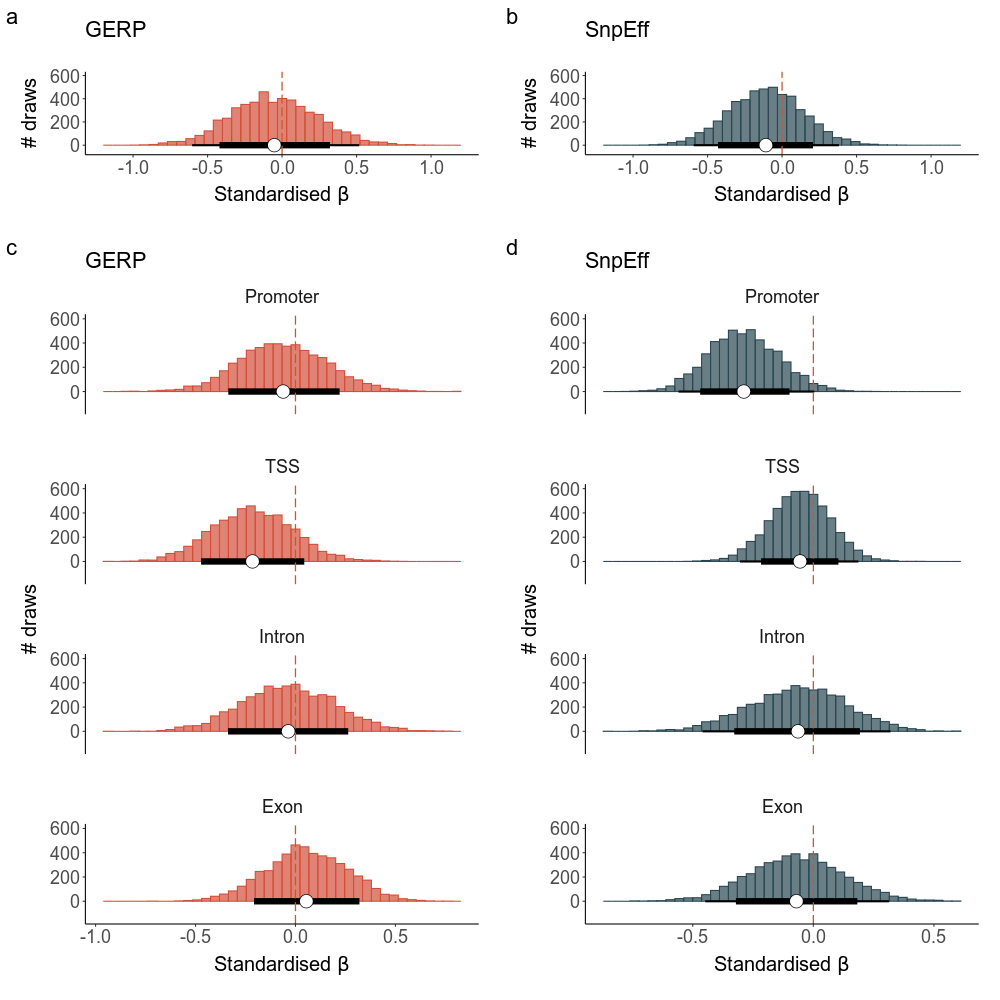
\includegraphics[keepaspectratio]{qmd/../plots/sup/sup_3_random_draws.png}}

}

\caption{Random subsets}

\end{figure}%

\bookmarksetup{startatroot}

\chapter*{References}\label{references}
\addcontentsline{toc}{chapter}{References}

\markboth{References}{References}

\printbibliography[heading=none]





\end{document}
